\documentclass[12pt,report]{memoir}
\usepackage{mempatch}
\chapterstyle{thatcher}

\settrimmedsize{11in}{8.5in}{*}
\settrims{0in}{0in}
\settypeblocksize{9in}{6.5in}{*}
\setlrmargins{1in}{*}{*}
\setulmargins{1in}{*}{*}
\setheadfoot{\onelineskip}{2\onelineskip}
\setheaderspaces{*}{1.5\onelineskip}{*}

\checkandfixthelayout

\let\footruleskip\relax % for compatibility of memoir and fancyhdr
\let\sl\ttfamily        % for compatibility of memoir and blindtext (silly, but it works)

\let\tt\ttfamily
\let\rm\rmfamily
\let\sc\scshape
\let\bf\bfseries
\let\it\itshape

\usepackage{fancyhdr}
\pagestyle{fancy}
\fancyhead{}
\fancyfoot{}
\cfoot{\thepage}
\renewcommand{\headrulewidth}{0pt}

\usepackage[usenames,dvipsnames]{color}
\usepackage[colorlinks,urlcolor=black,linkcolor=black,citecolor=black]{hyperref}

%% THINGS HERE
\usepackage{ccicons}
%% THINGS FROM PM AUTHORS:

%\usepackage[OT2,T1]{fontenc}
\usepackage[english]{babel}
%\usepackage[latin1]{inputenc}
\usepackage{amssymb}
\usepackage{amsmath}
\usepackage{amsfonts}
\usepackage{amsthm}
%\usepackage{html}
\usepackage{graphicx}
\usepackage{fancyvrb}

%
\DeclareMathOperator{\Tr}{Tr} % needed as example
\newcommand*{\BibTeX}{{\rm B\kern-.05em{\sc i\kern-.025em b}\kern-.08em
 T\kern-.1667em\lower.7ex\hbox{E}\kern-.125emX}}
\newcommand*{\Xy}{{\kern-.1em X\kern-.3em\lower.4ex\hbox{Y\kern-.15em}}}

%\begin{htmlonly}
\renewcommand*{\BibTeX}{Bib\TeX}
\renewcommand*{\Xy}{Xy}
%\end{htmlonly}

%% LOADING LAST:
\usepackage{memhfixc}

\begin{document}

\renewcommand{\abstract}[1]{\begin{center}\begin{quote}
\emph{#1}
\end{quote}\end{center}}

\title{PlanetMath Documentation}
\author{Joe Corneli\thanks{Often recycling work by others under the terms of \ccbysa.}}

\begin{titlingpage}
\maketitle
\end{titlingpage}

\frontmatter

\renewcommand{\cftchapterfont}{\scshape}
\renewcommand{\cftchapterpagefont}{\scshape}

\tableofcontents*
\cleardoublepage

\mainmatter

\chapter{The PlanetMath FAQ}
\abstract{This based on the FAQ, written by mathwizard et
  all, which is available in its legacy format at
  \url{http://planetmath.org/?op=getobj&from=collab&id=35}.}

\section{General Questions}
\subsection{What is PlanetMath?}
PlanetMath is a free, collaborative, online mathematics encyclopedia. The stress is on peer review, rigour, openness, pedagogy, real-time content, interlinked content, and community-drivenness.

\subsection{Is PlanetMath anything like Wikipedia (or wiki software in general)?}
Yes. PlanetMath contains a set of interlinked concepts which derive meaning from both their content and their connections.  The interlinking is exposed as hyperlinks.  The ``meaning'' of a node is not just its textual content, but also its position in the network.  

But PlanetMath is different from wikis in some important regards.  First and foremost, the default model of content authorship is that of object ``ownership'', where a single person acts as the gatekeeper to the object's content.  However, you can also make your articles world-editable, or editable only by a specific set of co-authors.

\subsection{Is PlanetMath competing with MathWorld?}
PlanetMath was started in 2001, when MathWorld was taken offline in the course of legal proceedings against its author.   At that time, we assumed that there would be no MathWorld anymore.  The goal was then not to compete with MathWorld, but to make up for its absence with something that wasn't susceptible to the same pitfalls. 

In order to generate a lot of content quickly and efficiently, it was obvious that collaboration was needed, so this made PlanetMath a horse of a different colour right from the start.  Now that MathWorld is back, you have at least two choices for finding mathematical reference material online.   We believe PlanetMath is more attractive to contributors because of our open licensing policy.

\subsection{How do PlanetMath's goals differ from MathWorld's?}
Both PlanetMath and MathWorld have as a goal to be a comprehensive online encyclopedia of mathematics.  PlanetMath is built for collaborative authoring and peer-review.  It is a ``bazaar'' instead of a ``cathedral'' (if you're into \htmladdnormallink{Raymondite}{http://catb.org/~esr/writings/cathedral-bazaar/} terminology).  The guiding philosophy of the site's design is that the community can ``police itself.''

Another important goal of PlanetMath is to be immune from the courtroom, and to provide agreeable intellectual property rights to contributors.  This is achieved through the Creative Commons Attribution-ShareAlike license, which allows contributors to retain rights to their contributions, and allows PlanetMath.org (and others) to retain rights to a copy.

This approach shifts emphasis to be on sharing knowledge.

\subsection{Is there a downloadable version of the PlanetMath encyclopedia?}
There should be.  Historically, a daily snapshot of the website, containing both LaTeX, HTML, and PDF has been available.   Right now the snapshot-generating system is broken.

The content of the site has also been made available as a large PDF file suitable for printing (if you have a lot of paper).  However, this hasn't been attempted in a while.  You can still find copies of the Free Encyclopedia of Mathematics online, however, and new versions will be created when we have time.

\subsection{Do I need to know \TeX/\LaTeX{} to write a PlanetMath entry?}
It's strongly recommended. However, \LaTeX{} is not hard to learn, and we have 
provided an easy way to view the source code of any existing PlanetMath entry
to faciliate learning how to write mathematics in \TeX .  A PlanetMath-specific \LaTeX{} guide can can be found as a ``Site Doc''.

There are also quite a few good online references and tutorials for TeX and LaTeX:
\begin{itemize}
\item \htmladdnormallink{Getting Started With \LaTeX}{http://www.maths.tcd.ie/~dwilkins/LaTeXPrimer/}
\item \htmladdnormallink{Hypertext Help with \LaTeX}{http://www.giss.nasa.gov/latex/}
\item \htmladdnormallink{The Harvard Guide to \TeX}{http://abel.math.harvard.edu/computing/latex/manual/texman.html}
\item \htmladdnormallink{A Guide to \LaTeX}{http://www.astro.rug.nl/~kuijken/latex.html}
\item \htmladdnormallink{The Not So Short Introduction to \LaTeX2e}{http://www.ctan.org/tex-archive/info/lshort/english/lshort.pdf}
\end{itemize}

\subsection{Who can contribute?}
Anyone can make an account and immediately start creating entries.  Of
course, if you can't take constructive criticism, you might want to
reconsider.

\subsection{Who reviews content, and how?}
Anyone who wants to. The chief means of peer review is via the corrections system. Anyone can submit corrections (of type addendum or erratum) to any entry. Points are given for accepted corrections, providing a means of crediting the reviewing party's contribution.

It is up to the author to determine of a correction is worth accepting. However, corrections are always available for viewing. If a correction is either wrongly accepted or rejected, others may notice this and file further corrections.

\subsection{Who owns contributed material?}
The authors of content retain all rights they posses by law.  By joining PlanetMath, they also agree to license to PlanetMath all content they submit to the site.  Under this arrangement, authorship recognition must be preserved, but aside from that, anybody can make digital copies, print versions, or hard copy duplicates.  Anybody can set up their own web site with content from PlanetMath.  Anybody can sell compilations of that content.  For more details, see the Creative Commons Attribution-ShareAlike license.

\subsection{How can I help the project -- financially or otherwise?}
Please see our page on supporting PlanetMath.

\section{Usage Questions}
\subsection{How can I contribute?}
\begin{enumerate}
\item Make an account.
\item Browse around, get a feel for the site.
\item Read the New User \htmladdnormallink{documentation}{http://aux.planetmath.org/doc/}.
\item Log in, click on ``Encyclopedia'' under ``add'', in your user box.
\item Write your entry. Have a \LaTeX{} guide handy, if you don't already know \LaTeX{}.
\item Preview, submit. 
\end{enumerate}

\subsection{How do I know what content has already been added?}
You don't really need to, other than to avoid directly duplicating a concept someone else has already written an entry for.  However, this can be avoided by simply using the search engine. In addition, the system will provide a warning at entry-adding time if the title of your entry is suspiciously similar to the title of an existing entry.

Aside from this, many people are worried about how they can possibly hyperlink their entries to others without knowing which things have been defined in PlanetMath already. Luckily you don't have to know this at all -- PlanetMath is designed to do the reference linking between entries automatically, and instantly.

This works both ways: not only will your entries immediately link to existing PlanetMath entries, but when new entries are added for concepts mentioned in your entry, your entry will actually be updated to link to them. The end result is that each person can be ignorant of the contents of the actual corpus (up to intent to add new entries.)

For more information about the automatic reference linking, see the expository document on \htmladdnormallink{Automatic Reference Linking}{http://planetmath.org/?op=getobj&from=collab&id=32} and the \htmladdnormallink{User Linking Controls}{http://planetmath.org/?op=getobj&from=collab&id=33} guide.

The reason this system works is that the particular content of PlanetMath is not novel -- it's all concepts that have already been thought of, that are well-known, and that are known by consistent handles. In general semantic net frameworks where new knowledge is formulated, there is less of a need for automatic linking, and this is less possible since concepts don't have well-known handles. Hence this isn't a big priority for ``brain-storming'' type Wiki-systems.

\subsection{How do I view the \TeX{} source of an entry?}
Use the Source tab that comes with every article.

\subsection{How do I include diagrams in my entry?}
For diagrams, it is preferable to utilize a logical, description-based format, instead of a raster image (array of values representing pixels.)  In the \LaTeX\ world, the most useful of these formats are \Xy-pic, pstricks, and Tikz, but support for these formats is currently only partial in PlanetMath.  Feel free to experiment, but beware that some features might not work yet.

For now, the safest way to get images to show up will be to upload web-friendly graphics (JPG, PNG) to the gallery, and then include them in your document by writing:
\begin{verbatim}
\includegraphics{FILENAME}
\end{verbatim}

\subsection{I am having trouble reading an entry because the \TeX{} is not displaying correctly.  What do I do?}
Post a comment and we'll look into it.


\chapter{Community guidelines}

\section{New User Guide}
\subsection*{Before You Begin}
We are working to make PlanetMath into a consistent, correct, and
comprehensive, free mathematical resource.

When we say ``free'', we are refering to \emph{freedom}, not price.
The PlanetMath encyclopedia is released under the GNU Free
Documentation License (FDL). Using this license for your work means that
other people around the world will be able to copy and modify your
contributions in ways you hadn't necessarily imagined.

In order to be an effective PlanetMath contributor, you should be
aware of the responsibilities you take on when contributing.

One important responsibility is to only contribute your own writing,
or other texts that you know you have a legal right to add. The last
section of this document is about copyright, and it is important that
you understand the issues presented there. The other sections of this
document will help you understand the way the site works, and how to
write good entries.

One thing to bear in mind is that while we want our work to be
consistent and correct, it is not expected that you get things perfect
the first time. On the contrary, writing a correct and complete entry
is an iterative process. We caution you against expecting to be
precisely and exhaustively correct on your first (or second, or third)
attempt! You should not be afraid of receiving corrections and
suggestions from others, and in fact you should expect them.

Do not expect to retain ``ownership'' of your entries if you will not
have time to maintain them. There are plenty of people who will be
willing to adopt abandoned entries. If you do not respond to
corrections in a timely fashion, your entries will eventually be
considered to have been abandoned, and they can then be adopted by
someone else
(for details see
section ``The Adoption System'' in
\htmladdnormallink{Noosphere's Authority Model}{http://planetmath.org/?op=getobj&from=collab&id=34}
).

Part of the benefit of PlanetMath is the collaborative nature of the
project: math enthusiasts from all over the world want to share what
they know, and learn through sharing and discussion. If you do not
expect to learn and think you know it all beforehand, PlanetMath is
probably not for you.

\subsection*{Metadata}
\textit{Metadata} is a word meaning ``data about data''. For our
purposes, this means information about the main (\LaTeX) content of
your entry. Much of this document is about metadata for PlanetMath
entries. This includes titles, synonyms, defines (sub-definitions),
type, keywords, and classification.

To make your entry properly fit in with the rest of PlanetMath, it is
important that you understand how to best write its metadata. This is
not complicated, but perhaps not obvious to beginners, so read on to
see how.


\subsubsection*{Naming Your entry}
There are a few entry naming conventions that have evolved so far
which go a long way towards making PlanetMath a cohesive and
consistent resource. Some of these are purely issues of style, but
many have to do with the dynamics of linking between objects. Note that
they also apply to other ``concept labels'' --- synonyms and defines.

Here are the rules for naming your PlanetMath entries:

\subsubsection{Capitalize for indexing}
It is convention to capitalize your title as you would want it to appear in an index or list. Generally, this means that only proper nouns and adjectives derived from proper nouns are capitalized.

\subsubsection{Do not use articles}
Do not start entry titles with ``the'', ``a'', or ``an''. Articles add
no useful information to your entry names.

\paragraph{Examples.}
\begin{description}
\item[the binomial theorem]
Wrong, should be ``binomial theorem''.
\item[the bridges of Koenigsburg]
Wrong, should be ``bridges of Koenigsburg''.
\item[a proof of the binomial theorem] Wrong, should be ``proof of the
binomial theorem'', or ``proof of binomial theorem'', or ``binomial
theorem, proof of''.
\end{description}
Not only do we not want (for instance) a ton of entries appearing
under "T/the ..." in the encyclopedia's index, we also do not want
"the" to be hyperlinked in the body of the entries. (The same goes
for other articles.)

\subsubsection{Do not put subjects or sub-disciplines in titles}
For homonyms (ambiguous terms like ``algebra'', ``domain'', or
``complex''), it often seems appropriate to append a parenthesized
``subject hint''. For example, one might think the smart thing to do
is name an entry ``diagonalization (Cantor)'' to avoid conflation with
the linear algebra sense of ``diagonalization''. However, the way this
should officially be handled is to assign an appropriate subject
classification to your ``diagonalization'' object.

Adding a parenthesized ``subject hint'' to your title is acceptable
provided the plain title is at least given as a synonym (and the entry
is still properly classified.) You might want to do this with the
encyclopedia index listing in mind (that is, it might be nice to see
``diagonalization (linear algebra)'' in the index.)

\paragraph{Example.}
\begin{description}
\item[diagonalization (linear algebra)] Usually wrong, should be
``diagonalization'', and classified somewhere in MSC area 15 (linear
and multilinear algebra)
\end{description}

\subsubsection*{Classification}
You had a hint already of one reason why classification is important:
homonyms abound. There are a large number of terms in mathematics that
are ambiguous: you cannot tell from the term itself which concept is
being referred to, and you need some sort of context (or semantic
hint.) Classification serves this purpose well. In addition,
classification allows entries to be browsed by subject, through a
subject classification hierarchy.

For classification, currently PlanetMath only supports MSC, the AMS
Mathematical Subject Classification scheme. MSC is very widely used
and is more or less exhaustive over known mathematics -- you probably
will never run into an entry that can't be classified with MSC (at
least to one level in the hierarchy.)

The MSC takes some getting used to. In order to make things easier, we
have set up a \htmladdnormallink{local copy}{http://aux.planetmath.org/msc}
of the MSC which is hierarchically browseable and searchable, which
is accessible from the menu.

\subsubsection*{Types}
There are a number of types which are available for describing what
the mathematical form of your entry is. These are:
\begin{itemize}
\item Definition
\item Theorem
\item Conjecture
\item Axiom
\item Topic
\item Biography
\item Algorithm
\item Data structure
\item \textit{Proof}
\item \textit{Result}
\item \textit{Example}
\item \textit{Derivation}
\item \textit{Corollary}
\item \textit{Application}
\end{itemize}
The entries in italics are meant to be attached to other entries. They
do not show up in the encyclopedia index, so placing an entry under
one of these categories has important practical as well as
philosophical ramifications.

An example of why types matter: a definition should not have proof,
since definitions have no truth value -- but it may have a
derivation. Hence, you cannot attach a proof to a definition
(actually, you can, but it is discouraged.)

A theorem may have a proof, and in fact it should be provided for a
full acceptance of the theorem as a theorem. Hence, PlanetMath makes
it easy for a proof to be attached to a theorem (and only a theorem.)
As before, you actually can attach a theorem to anything, but doing so
is less convenient and is discouraged.

Examples are meant to be used everywhere. They allow some of the load
to be taken off the primary entry author, by allowing the community of
users to pedagogically enrich existing entries.

The ``Conjecture'' type might be a little confusing to some. In terms
of how the system treats conjectures, they are the same as
theorems. That is, they are meant to have proofs attached to them, as
well as results or corollaries. This makes sense, since a conjecture
is basically treated as a yet-unproven theorem. However, when one
looks at a topic like the Taniyama-Shimura conjecture (which has now
been proven), its hard to decide which type is more
appropriate. Proven conjectures may still be better left as
conjectures by convention. The opposite situation is a conjecture
which is considered a theorem before its time -- like Fermat's last
theorem. Yet another situation might occur when it turns out a
conjecture (like the Continuum Hypothesis) is unprovable (can only be
used as an axiom). There is no single answer for these situations, you
simply must take into account practical considerations (for instance,
that conjectures won't show up in ``unproven theorems'') and
convention on a case-by-case basis. Don't worry too much, however,
about picking the absolute best type the first time around in such an
ambiguous situation.

\subsubsection*{Synonyms and Definitions}
PlanetMath provides a ``synonym'' field for entries. The obvious
things to put in here are alternate names for your entry. The
not-so-obvious thing is that you should also be thinking of linking
when you do this. That is, you should list all aliases for your entry
that someone else might invoke in other entries, to faciliate
automatic linking.

You do not, however, need to make extra synonyms for variants of
pluralization, possessiveness, or transmogrifying ``Blah, proof of''
into ``proof of Blah''. \emph{These are done automatically by
PlanetMath.}

\paragraph{Examples.}
{\bf title:} \emph{Euler's totient function}, {\bf synonym:}
\emph{Euler totient function}. Wrong -- the synonym is just the
nonpossessive of the title; leave that for the software to handle!

{\bf title:} \emph{Cauchy-Schwarz inequality}, {\bf synonym:} \emph{Kantorovich's inequality}.
Correct -- both names are used to refer to the same thing.

{\bf title:} \emph{monotonic}, {\bf synonyms:} \emph{monotone,
monotonically}. Correct -- we want all occurrences of ``monotonic'',
``monotone'' and ``monotonically'' to link to the same object.

{\bf title:} \emph{vector valued function}, {\bf synonyms:} \emph{vector-valued,
vector-valued function, vector valued}. Correct -- we have to take care
of variants in hyphenation as well as the particular set of words.

In addition, there is a ``defines'' field which provides for
``sub-definitions'' of your entry. This facility allows you to define
some set of new concepts all at once in a single entry (for example,
it might be better to define ``edge'' and ``vertex'' within a
``graph'' entry, instead of separately). Each of these
``sub-definition'' handles will be treated appropriate by PlanetMath's
automatic linking when they are invoked in other entries (they will
get hyperlinked, whereas multiple synonyms to the same entry will
not.)

Previously it was the case that ``synonyms'' were used to list these
``sub-definition'' concept handles. This is no longer the case. The
two types of handles have different ramifications for linking, and
deserve to be separated.

\paragraph{Examples.}
\begin{itemize}
\item An entry for ``graph'' may also define ``vertices'' and
``edges'' and hence have ``vertices, edges'' as the ``defines''
field.
\item An entry for ``Zermelo-Fraenkel axioms'' may also list as
sub-definitions each individual axiom, i.e. defines=``axiom of empty
set, axiom of infinity, ...''
\item An entry for ``Taniyama-Shimura conjecture'' might also have
synonyms ``Taniyama-Shimura-Weil conjecture'', ``Taniyama-Shimura
theorem'', and ``Taniyama-Shimura-Weil theorem'', and hence list
these as synonyms. These would not be listed in the ``defines''
field -- if two of these terms are invoked from the same entry, they
should not both be linked, which will be the case if they are listed
as synonyms.
\end{itemize}
It is important to note that there is no general rule for the exact
``granularity'' of entries -- things that ``stand on their own''
should be their own entry, but this is hardly a rigorous metric
(however, if you choose to combine things that could be separate
entries, you should provide a ``defines'' list for sub-definitions.)
Use your best judgement, and you'll probably hear from others if
there's disagreement.

\subsection*{Corrections}
What you should file corrections for:
\begin{description}
\item[Mathematical Errors] These may be as simple as a typo or as
serious as a completely erroneous proof.
\item[Typographical errors and grammatical errors] PlanetMath should
be as ``professional'' as any published book or encyclopedia (in
fact, there is little excuse for the quality of PlanetMath not to
exceed fixed media for the set of ``stable'' entries.) As such,
please point out even the smallest of mistakes, if they truly are
mistakes.
\item[Comprehensiveness] If more can be added, it probably should
be. This includes showing relatedness to other branches of
mathematics, and possibly applications. It includes alternate
derivations, additional results and properties, and different
methods of visualization or approaches to explanation. You don't
have to write a book -- that would of course defeat the purpose of
an encyclopedia. But the idea is to mention all of the important
insights so that the reader knows what to look for if they'd like to
study the idea in more detail.
\item[Comprehensibility] Formal and concise statements tend to be
useful for reference purposes, but they are not very useful for
learning what one does not already know. More extensive
explanations, visualizations, and examples are very powerful tools
for teaching, and they should play a large part in nearly all
entries.
\item[Alternative conventions] This is a tough one for most. Often
times there are conventions which vary from country to country,
region to region, school to school, or even class to class. Think of
PlanetMath in a global context when you write and critique entries,
and it should become apparent that probably most alternatives should
at least be mentioned, before a particular choice is made for usage.
\item[Interconnectedness] By this we mean provisions for making
PlanetMath as interlinked as possible. This includes tweaking
mentions of concepts so that they trigger linking to a PlanetMath
entry, or conversely, adding synonyms to entries or tweaking titles
to conform with the way they are mentioned in entries. It includes
adding explicit ``related'' (See also) links to other things in the
encyclopedia when they should be there. Also important is reporting
to an object owner when a link goes to the ``wrong'' entry, or there
is a link where there should not be, and reporting the lack of a
subject classification (which serves as a hint to automatic
linking).
\end{description}
Likewise, you should expect to receive corrections when your entries
are lacking in any of these areas.

Corrections don't always go smoothly. Often you feel a correction was
justified, but the author rejects it. The first thing to do in this
situation is find out if there was a misunderstanding: you can post
messages to the correction and discuss it. You can try filing another
correction wording things differently. When it becomes clear the
author is not going to do things your way, we suggest the approach
from the next section. \textbf{Under no circumstances will the staff
of PlanetMath mediate disagreements about corrections.}

\subsection*{Alternate Entries}
You should always run a search before writing an entry to see if
someone else has already covered the same material. However, even if
the ideas have already been discussed, there may still be reason for
you to write an alternate entry. Alternate entries are justified when:
\begin{itemize}
\item you have a radically different treatment of the subject. This
could be another educational level (as in introductory
vs. advanced), or another method (as in a proof, which can have tens
of alternatives).
\item the author of the entry is discarding corrections. In this case
the object will not eventually be orphaned for pending corrections,
so you cannot force modifications to it (do \textbf{not} complain to
the staff in this case; we won't force the other author to do
anything).
\end{itemize}
We would prefer uniformity and cohesion on PlanetMath, but there is a
natural limit to how far this can be stretched with so many different
minds. The lack of scarcity (i.e. limited space) on PlanetMath also
gives it an advantage over traditional media, allowing us to avoid
standardization and provide extra value in yet another way.

\subsection*{Copyright}
While mathematical concepts can not be owned, their expression is
subject to the strictest protection under copyright law. Furthermore,
one cannot convey mathematical information without expressing it
somehow. There is much more to ``expression'' than simply an
author's choice of words and, accordingly, direct copying is only one
of many sorts of copyright infringements.

Below, we present some guidelines for writing entries that may help
you avoid exposing yourself or PlanetMath.org to legal problems.

\begin{itemize}
\item Bear in mind that a text does not need to have a copyright
notice attached to it in order to be copyrighted. Moreover,
copyright protection has nothing to do with whether the work is
published or unpublished, whether a work is still in print, or
whether the publisher charges for copies of the work. In fact, the
simple act of writing something down automatically confers copyright
protection to the author. In particular, this means that class
notes and handouts, webpages, and newsgroup postings are all legally
protected.
\item If you see the exposition of a certain mathematical topic on
someone's homepage and think it would make a great addition to
PlanetMath, you should do nothing unless you can first obtain the
copyright holder's permission, in writing, to publish a copy of the
work on PlanetMath. Likewise, you may not post a copy of notes that
were handed out in a class, or even notes that you took on a spoken
lecture, without first obtaining written permission. Asking for
permission is also an opportunity to tell others about PlanetMath
and the FDL. However, if you do not receive the author's permission
to publish under FDL terms, you cannot post the work! If you do
receive the copyright holder's permission to use the work,
\emph{include their permissions statement as an attachment.}
\item When dealing with published material, especially if it is still in
print, keep in mind that authors sign contracts with their publishers
which typically restrict the author's rights. Therefore, even if the
author of a book or an article in a journal gives you permission to
use his work, it may be and likely will be necessary to also obtain the
publisher's permission.
\item Copying from FDL'ed works is fine, but it requires us to follow
a special protocol -- if you would like to copy from an FDL work,
please post in the forum, so a site administrator can review the
work's license and then take the necessary steps.
\item Copying from public domain works is also fine. Mathematical
works that are in the public domain are mostly those whose
copyrights have expired, but also works that have been transfered to
the public domain by their authors, as well publications of the US
government. As a rule of thumb, works published in the ninteteenth
century and earlier are in the public domain, but unless you can
find proof to the contrary, twentieth century works are likely to be
off-limits. It is of course wise to give a citation so that others
can easily check the assignment (or expiry) of copyright for
themselves -- and perhaps also find additional useful material from
the same source.
\footnote{When dealing with older works, keep the following points in
mind: (a) The law on when copyright expires is somewhat different
for unpublished works, so these need to be treated as a special
case; (b) Before World War II, English was not the dominant language
of the mathematical community. Therefore, older works are more
likely than contemporary works to appear in a language other than
English. Since translation is a creative act, translations are
protected by copyright, even if the work that was translated is in
the public domain. Thus, if you quote at length from an older work
written in a foreign language, you should either do the translation
yourself, or else find a translation which is also in the public
domain (or FDL'ed).}
\item As a rule of thumb, if you cannot provide at least a sketch of a
given topic without referring to a source, you are probably not yet
qualified to write an entry about that topic. Not only is this
policy prudent from the legal standpoint, it also makes sense from the
point of view of mathematical content. If you rely too heavily on a
given source, you run the risk of perpetuating whatever mistakes and
oversights may be present there. Furthermore, unless you have a
fairly deep understanding of a given topic, you might misunderstand
another author's use of a particular technical term, or forget to
state assumptions which this other author stated in an earlier
chapter. A document written from your own understanding will be much
more useful than one that purports to present facts that you
yourself do not understand. You needn't be a world expert to write
a useful entry -- simply trying to state your own questions clearly
will be much more helpful to everyone involved than it would be for
you to try to mimic someone else's exposition.
\item Cite all sources, including any web pages, lectures, or personal
communications that have informed your work. If possible, summarize
the relationship your article bears to the source or sources you
used. Which parts of the article derive from which sources? Which
parts are original?
\item Keep in mind the fact that, as the copyright office says,
``Acknowledging the source of the copyrighted material does not
substitute for obtaining permission.'' To be sure, documenting the
process you used while writing an article, and which sources you
looked at, could help prove that you did not infringe on anyone
else's copyright -- but whether or not you cite a particular work is
not a factor in determining whether your work infringes on that
work's copyright.
\item Embellish your articles with examples, illustrations, proofs,
and other extensions either of your own devising or drawn, bit by
bit, from a variety of sources -- make your exposition truly your
own. No one part of your article should be too close to anything
drawn from any one source. In addition, neither the overall
structure of your article nor any part of its structure should be
too close to the structure or any non-trivial part of the structure of
any one source.
\item Bear in mind that the particular choice of words that an author
uses is not the only thing that copyright protects: copyright
protects expression in general, and even the particular selection of
facts or ideas that an author chooses to talk about is protected.
\item However, copyright does not protect individual facts, ideas,
concepts -- so write about all these things! But always do it in
your own words, and do not rely too heavily on one source. Even
something as simple as a theorem statement or a non-trivial equation
should be put in your own words, and expressed in a way that is
consistent with other usage on PlanetMath.
\end{itemize}

PlanetMath staff will \emph{not} protect entry authors from the
consequences of any copyright infringement, and rather will do
everything in their power to protect the site from the irresponsible
(though perhaps well-intentioned) actions of persons who seek to
contribute things they do not have the right to.

We do encourage you to find content written by others that you have
been given permission use as part of PlanetMath. As mentioned above,
a special protocol must be followed in order for us to use works that
have been released under the GNU FDL. In particular, if you are
adding material from a GNU FDL source that hasn't already been listed
on PlanetMath's History page, an appropriate item will have to be
added there; thus, if you are planning to upload all or part of an
FDL'ed source, or a modified version thereof, you should get in touch
with the site administrators first.

When it comes to deciding whether some particular use of a copyrighted
source is permissible, the distinction betwen a \emph{derivative work}
and \emph{transformative use} needs to be kept in mind. While there
is no space here to go into details and study examples, at least a
brief description should suffice to make the reader aware of the legal
principles that are in play here, and the fact that there is an
important distinction between the two kinds of use.

A \emph{derivative work} is one whose content has been derived from an
already existing work. Examples include translations, abrigements, or
adaptations. Even though a derivative work can contain a substantial
changes or additions of new material and other original contributions,
a derivative work cannot be prepared without the permission of the
owner of the copyright of the original work on which it is based. (In
fact, minor changes and additions to an existing work do not even
qualify as derivative work, but rather as outright copying.) The FDL
gives users permission to publish derivative works, so long as the
derivative works are released under the terms of the FDL. In general,
non-FDL'ed copyrighted works offer no such permission to their users.

In contrast, \emph{transformative use} of copyrighted material
consists of putting the material to a different use or function than
that originally intended by the author of the original work. This is
permitted as a fair use of copyrighted material but one needs to be
careful not to take any more of the material than is necessary for
this new purpose. In deciding whether a certain usage is suitably
``transformative'', one consideration is whether or not the new work
affects the marketability of the old work, or whether it in fact
satisfies a purpose for which the original work was designed.

One needs to remember that in deciding a copyright infringement case,
courts will consider how much material may have been used without
permission. Thus, it may be OK to have a single short entry that is
rather close to the small section of an original work from which it
derives; however, it is a more serious matter if a whole series of
short entries are all based on the same source.

For further discussion of copyright issues or questions, please use
the \htmladdnormallink{forums}{http://planetmath.org/?op=forums}.

\subsubsection*{An Important Note On Using MathWorld}
In addition to the copyright guidelines above, a few more words need
to be added concerning MathWorld.

In short, we strongly suggest \textbf{not using MathWorld at all} in
the process of researching an entry, and furthermore we suggest not
linking to it in your articles.

The owners of the copyright on the MathWorld content have a proven
track record of aggressively defending their copyright. It is simply
not worth the risk, even when you feel sure you'd only be making fair
use of things you found there. Not only will this policy help us
avoid potential legal snares, it will help to solidify in the minds
of readers the difference between the two sites.


\section{PlanetMath Community Guidelines}
This guide spells out some of the ground rules on how users should
interact with each other on PlanetMath, whether in the PM Forums, or via PM Encyclopedia contributions, or other areas of the site. In a nutshell, the ground rules ask that the users be respectful and considerate of one another. More specifically, the ground rules are as follows:

\subsection{With regard to posting on PlanetMath}
\begin{enumerate}
\item Try to stay on the subject of mathematics, or things related to PlanetMath.
\item No ``spamming'' or ``shilling''.  Whilst informing the community of events, publications, software, and the like which are of interest to mathematicians and discussing their relative merits  is acceptable, the PlanetMath website is not to be used for promoting or advertising products, services, or events.
\item Since the website is used by children learning math, only use laguage suitable for a general audience in public areas; no profanity, obcsenity, or off-color jokes, please.
\item When referring to other individuals (persons or entities), be respectful and complimentary.
\item If you don't have anything good to say, sometimes the best course of action is to say nothing.
\item If you do have disagreements and want to discuss it in public, do it in a constructive manner. Try not to make judgment or use sarcasm in any negative way. Do not make unfounded accusatory comments. Avoid starting a flame war.
\item When asking for help or posing a question, do not expect that someone else will do all the work for you or hand you the answer on a silver platter.  Instead, consider showing your work, indicating where you are stuck, and be willing to work alongside someone giving help since such an approach is more likely to arouse sympathetic interest.
\end{enumerate}

\subsection{With regard to a filing a correction notice to a PlanetMath entry}
\begin{enumerate}
\item If you have an issue with an entry, file a correction notice first. Explain why you have an issue, and point out any possible course of action for a solution if you know one. Be polite and to the point.
\item If the correction is not done to your satisfaction, you may consider filing another correction notice.
\item Try to resolve the issue peacefully with the author of the entry. 
\item Or, you may consult the rest of the PlanetMath users for additional input. Do so in a constructive manner.
\end{enumerate}

\subsection{With regard to writing and maintaining a PlanetMath entry}
\begin{enumerate}
\item If you are knowledgeable about some math concept and do not find it on PlanetMath, or if you know an alternative way of describing a concept (or proving a proposition) that already appears on PlanetMath, feel free to contribute an article/entry on it.
\item On the other hand, if you are not knowledgeable about the concept, and still like to see it on PlanetMath, file an entry request so others may contribute.
\item Also, consider collaborating with others if the task of writing an entry alone is too great. Make the entry world-editable if necessary.
\item  When relying on other sources for information or exposition, follow the norms of scholarly ethics in giving credit where it is due.  Do not claim credit for ideas or work which you did not produce yourself.
\item Even if you are wtiting an entry based completely upon your own understanding, please consider adding bibliographic references and website links so as to provide further reading for people interested in learning more about the topic.
\item If you would like to fill a pending request or adopt an orphaned/abandoned entry and feel that you do not have adequate knowledge regarding the subject matter, please consult the PM public or the requester for more information first, or
\item Better yet, be considerate and leave the requests and orphaned/abandoned entries alone so others who are more knowledgeable can take care of the request/orphaned entry.
\item Consider giving up an entry to others either by transferring, orphaning/abandoning, or turning it world-editable, if the task of owning an entry is too great, or there is no time at the moment to take care of filed corrections.
\item Please take care of outstanding correction notices in a timely manner. The PM system will issue nagging email if an outstanding correction notice has not been taken care of for an extended period of time, and will orphan the entry that the correction notice is attached to if no action is taken.
\item Please do not keep entries with outstanding correction notices by transferring them back and forth between friends. 
\end{enumerate}

\subsection{With regard to diversity and disagreement}
\begin{enumerate}
\item The PlanetMath community is a diverse collection of individuals who
share a common interest in mathematics and make use of common
resources to promote this interest.
\item Because of the differences of backgrounds, interests, and abilities
between members of the community, there are bound to arise differences
of opinion. Handled appropriately, these differences can lead to
growth and be a source of strength and vitality for the community.
\item While it is perfectly legitimate to disagree with someone else, this
should be done in a productive manner. Merely stating disagreement is
not likely to accomplish much --- explain the reasons why you do not
agree and be specific as to the points of disagreement. This way
leads to dialogue which can resolve the disagreement rather than
fights which typically only entrench both sides in the conviction that
each side is right and the other side is wrong.
\item Do not take differences of opinion personally.
\item One side convincing the other side that it was wrong is not the only
way of resolving a disagreement. It is also possible that each
disputant will come to understand the other's point of view and both
will together come out with a new proposal which combines the good
points of both proposals but is not open to the objections which were
raised.
\item Be tolerant of others who may have different tastes, styles, and
interests. Do not object to something someone else is doing unless it
is causing harm. However, feel free to give and receive criticism as
long as it is done in a courteous, constructive fashion.
\end{enumerate}

\subsection{With regard to changes and improvements}
\begin{enumerate}
\item If there is something you would like to see happen at PlanetMath, work
towards making it happen. If it is a small thing and you have the
necessary skills, consider doing it yourself as time permits. If it
is a large project or you do not have all the necessary skills, do as
much as you can --- putting effort forth shows that you are serious
about making your proposal happen and therefore may serve to
interest others in participating.
\item While you can certainly try to interest others in what you are doing
and can expect that others should respect your choice of priorities,
no one else has an obligation to collaborate with you since
participation in PlanetMath is voluntary. In order to interest
others in helping you, you might want to consider offering to help
others and finding common ground with what others are doing.
\item If you would like to do something which is going to have at best
minimal impact on how others use the website, feel free to proceed.
\item If you would like to do something which has the potential to
significantly affect how others use the site, contact the affected
parties to discuss your plans and be prepared to modify your plans to
accommodate their needs and involve them in the planning process.
\item If you have an objection to something someone is doing or planning
to do, please raise that objection in a timely fashion. It is
disrespectful to wait until someone has already invested significant
effort towards a project to make known objections which would
have that person making significant changes to plans or undoing work
already done.
\end{enumerate}


\section{PM Rules of Compliance and Enforcement}
In this document, PM means PlanetMath, and PMCC (or CC for short), means the PlanetMath Content Committee. Since the document deals specifically with PM Content, issues related to PM Forums are not covered here.

This document refers only to those objects that are under the supervision of the CC, which include: encyclopedia entries, papers, books, expositions and requests (on the Requests List).

\subsection*{Offenses}

Offenses are usually brought to the attention of the CC via one of the following two channels: direct observation by CC, or complaint email from a PM user.\\

Offenses are classified by their severity:
\begin{enumerate}
\item A \emph{minor offense} is any one of the items below
\begin{enumerate}
\item failure to comply with a request by CC within the given timeframe, which includes
\begin{enumerate}
\item request to revise/reclassify objects
\item request for a type 1 object deletion
\item request to halt productions of new objects
\item request to halt updates of existing objects
\item request to halt adoption of orphaned entries
\end{enumerate}

\item any actions performed by the CC on behalf of the offending user, including
\begin{enumerate}
\item object reclassification
\item type 1 object deletion
\item object confiscation
\end{enumerate}

\item three valid complaint notices (such as inappropriate encyclopedia entry, etc...) received from PM users within 60 days. In order for a complaint notice to be valid, the offensive object has to be validated by CC, and then communicated to the owner of the entry.
\end{enumerate}

\item A \emph{moderate offense} is any one of the items below
\begin{enumerate}
\item three minor offenses by a user within 4 months
\item type 2 object deletion
\end{enumerate}

\item A \emph{major offense} is any one of the items below
\begin{enumerate}
\item two moderate offenses within one year
\item type 3 object deletion
\end{enumerate}
\end{enumerate}

\subsubsection*{A Note on Object Deletions}

There are three types of administrative object deletions, ordered in increasing severity:
\begin{enumerate}
\item type 1: an object deleted by CC due to the expiration of an object-deletion request made by CC to the owner of the offending object, for reason due to lack of clarity, lack of mathematical content, invalid request, etc...
\item type 2: an object deleted by CC due to the expiration of an object-deletion request made by CC to the owner of the offending object, for reason due to commercial spam, plagiarism, etc..
\item type 3: an object automatically (without notice to owner of the object) deleted by CC due to use of offensive language, personal threats, etc...
\end{enumerate}

\subsection*{Counting Offenses}

\begin{enumerate}
\item Offenses are partially cumulative. Each offense has an issue date and an expiration date. For a given offense, the time between the issue date and the expiration date is the life span of the offense:
\begin{enumerate}
\item a minor offense has a 6-month life span
\item a moderate offense has a 18-month life span
\item a major offense has 36-month life span
\end{enumerate}
After the expiration date of an offense, the offense is erased.
\item Offenses are convertible:
\begin{enumerate}
\item when three minor offenses are accumulated in a 4-month period, a moderate offense is generated with an issue date the issue date of the latest minor offense. In the meantime, the three minor offenses are erased.
\item when two moderate offenses are accumulated in a 12-month period, a major offense is generated with an issue date the issue date of the latest moderate offense. In the meantime, the two moderate offenses are erased.
\end{enumerate}
\item At most one offense per incident may be considered. An incident is a sequence of events that are related by a single CC request. For example, CC requests that a user deletes one of his entries, he fails to comply, and CC deletes the entry for him. The whole sequence of events is considered one incident. Although both the failure to comply with a request by CC (see 1.3.(a) above) and the subsequent deletion of the entry by CC (see 1.3.(b) above) are qualified minor offenses, only one minor offense may be considered.
\end{enumerate}

\subsection*{Consequences}

Every offense is associated with a sequence of penalizing consequences. Below are descriptions of these penalties and other administrative actions.

\subsubsection*{Penalties}

To each severity type of offense, there corresponds a choice of a variety of penalties of like magnitude for the offending PM user:
\begin{enumerate}
\item minor offense: either a warning issued by CC, or up to 1000 points deduction
\item moderate offense: either a short term (30-day) suspension, or between 1000 to 5000 points deduction
\item major offense: either an indefinite suspension, or between 20000 to 50000 points deduction
\end{enumerate}
Note: the number of points being deducted as a result of a penalty imposed should be at most the number of points owned by the offending user.\\

During an offense conversion, the offending user will be penalized for the offense being converted to, instead of the offense being converted from. For example, when the offending user receives the second moderate offense within a year, the two moderate offenses get converted into a major offense. As a result, the user receives penalties associated with the major offense, and not the second moderate offense that has now just been erased.\\

\subsubsection*{Other Actions}
In addition to receiving a penalty, there is usually an action (called a consequence) taken associated with the offending object (or objects). These consequences include:
\begin{enumerate}
\item administrative reclassification of an object
\item administrative confiscation of an object
\item administrative deletion of an object
\end{enumerate}

\subsubsection*{Reversibility of Consequences}
Certain penalties and administrative actions are reversible. For example, points deducted by CC, or deleted by CC can be reinstated. However, certain penalties are not. User account suspension, for example, is an example of irreversible penalties. CC has the discretion to reverse reversible actions. Nevertheless, CC should try to apply reversible penalties when possible, and reserve irreversible penalties for extreme cases. Also, offense conversion does not necessarily mean erasure of corresponding prior penalties, even if the penalties are reversible. Again, CC has the complete discretion over this matter.

\subsection*{CC Responsibilities}
If CC determines an offense has been committed by a PM user, it has the discretion to impose penalties on the offending user, and other actions on the offending objects. The following guideline shows how this is done:

\begin{enumerate}
\item First, CC will weigh on the severity of the offense, and decide whether it is worth pursuing the matter further with the offending user.
\item If CC decides to continue with the disciplinary action, an email notification must then be sent to the offending user (from PMAdministration), spelling out the offense the user has committed.
\item If CC decides to impose penalties and other actions, the specific penalties and actions must also be clearly spelled in the same email notification. These actions must be carried out in a timely manner.
\item All offenses and subsequent penalties and/or other actions must be documented in the Table of Disciplinary Actions.
\item If a penalty involves the suspension of a user account, CC must obtain approval from the PM membership enforcement committee first.
\item If an administrative action involves a type 1 entry deletion, the content of the offending entry must be saved (using get metadata) for documentation.
\end{enumerate}


\subsection*{Revisions}

\begin{enumerate}
\item Split from the ``original'' draft of the PM Community Guideline (11-11-2008) --[[CWoo]]
\item Major revision (2-4-2009) --[[CWoo]]
\item Added CC responsibilities Section (2-5-2009) --[[CWoo]]
\item Minor revision, changed ``entries'' by ``objects'' when appropriate (16-2-2009) --[[asteroid]]
\end{enumerate}


\section{Forum Policy}
\subsection*{Synopsis}

This brief document summarizes rules/regulations, conventions, and tips for using the PlanetMath forums.

\subsection*{Rules}

The rules for the PlanetMath forums are:

\begin{enumerate}
\item The forums are, for the most part, to be ``G-rated.'' So, no profanity, please. The only possible exception to the G-rated rule is the ``Humor'' forum, but please keep it to ``PG-13'' level here.
\item No flaming! How do you know if you are flaming? Basically, if you are arguing, not debating. Don't get emotional in the forums!
\item No spamming/commercial advertising! If you want to advertise on this site, buy Google ads. We keep the commercial and noncommercial stuff cleanly separated here.
\end{enumerate}

As you can see, the rules are few, and are pretty intuitive. However it is important to understand what makes these ``rules'' and not ``suggestions'': \textbf{if you break them, you are subject to enforcement} on this site. That means possibly getting locked out, having your account deleted and/or banned, and possibly losing control of any objects you own on the system. Enforcement is at the discretion of the administration!

\subsection*{Guidelines}

This section is for ``soft'' forum policy: guidelines, tips, and conventions. It is highly recommended that you follow them, but there is no administrative enforcement.

\begin{itemize}
\item When asking for help on mathematics, \emph{do not ask for the answer}. Nobody wants to do your work for you! Instead, state the problem and what you are confused about, and someone will almost certainly help you through it.
\item No ``shilling.'' Put another way, shamelessly self-(or otherwise) promoting advertising is frowned upon. However, it is ok to forward the bulletins of noncommercial math societies and the like.
\item Be polite, even when other people aren't! Be the more mature person! Messages that don't violate the rules will never go away; don't say anything you'll look back on and be ashamed of (of course, its ok and natural to be \emph{wrong}, but don't be \emph{mean}).
\end{itemize}

\subsection*{Updates}

Your help in developing this policy is welcome. Of course the administration has the last word on the rules, but feel free to add to the guidelines. Discussion of proposed changes to this document in the accompanying forum is recommended.


\chapter{Writing articles}

\section{PlanetMath Content and Style Guide}

\subsection*{Rationale}

This guide is meant to be a set of suggestions revealing the ``best way'' to write PlanetMath entries. One reason it is needed is because there are many common \LaTeX{} pitfalls that new or even intermediate \LaTeX{} writers may experience, and we hope to help them here. The second is because while there are many ways to do things both in terms of presentation style and \LaTeX{} use, we want to encourage writers to select the methods that will help make PlanetMath more consistent and hence easier to understand.

We stress again that this is only a guide---not a forced set of rules. The owner of an entry is assumed to be its expert, not the PlanetMath staff or any other users of the site. However we appeal to each and every writer to heed this document, to help make PlanetMath a better resource for all learners.

\subsection*{Content Guidelines}

What to write.

\subsection{Definitions}

In definitions, the term (or terms) being defined should be distinguished by typesetting it in either \emph{italics} (preferred) or \textbf{boldface}.
(See section \ref{sec:font-faces}.)

A basic definition-entry should give only one name and one notation (when such exists) for what is being defined. This will make the definition as short as possible and thus easy to read. It will also encourage a common notation/term for use at PM.

However, after the definition is given it is highly encouraged to mention examples, possible synonyms, alternative notations, etymology, and historical comments. These items could be placed in one or more additional sections, such as ``Examples'', ``Notes'',
``Properties'', and so forth. Lengthy examples should have their own entries attached to the definition.

Often an entry is lengthy, so that the definition might become difficult to distinguish from the surrounding text. This is especially noticeable if some introductory text precedes the definition. In such cases it is a good idea to somehow mark the definition so that it stands out. One way to do this is to use a ready-made ``definition'' environment (see below).

Sometimes, many concepts must be defined at once in a single entry. For example, it is difficult to define ``graph'' without also defining ``nodes'' and ``edges''. It makes more sense to group these things together. These additional concepts can be listed as defined in the ``defines'' metadata field of the entry. Synonyms for the main concept should be listed in the ``synonyms'' field.


\subsection{Theorems}
In theorems, it should always be clear what the assumptions
are and what are the implications. Also, one should try to eliminate
any unnecessary notation from the formulation. In particular, the
theorem formulation should not be used to set up the notation for
a proof. Such unnecessary notation will make the theorem difficult
to read.

As with definitions, if the theorem is surrounded with explanatory text (as most theorems should be), it is probably a good idea to set it off from the surrounding text in some way. A ``theorem'' environment (see below) is a good way to do this. Some publication styles set theorems in slanted text to attract attention.

\subsection{Proofs}

Proofs may be included in the entry for the theorem itself if they are
short; they should if possible be clearly marked as a proof, perhaps
by using {\tt \verb|\begin{proof}| \ldots \verb|\end{proof}|}
environment (see below). If the theorem contains its own proof, the
appropriate checkbox should be set, so that the theorem does not
appear on PlanetMath's ``unproved theorems'' list.

If the proof is long, it should go in its own entry, attached to the theorem itself. There's an ``add proof'' button for just this purpose. Others may attach alternative proofs to your theorems as well.

\subsection{Topics}

\subsection*{Style Guidelines}
How to write:

Since entries at PM are entries in an encyclopedia, each entry should
stand on its own.

\subsection{Logic symbols versus words}

Logic symbols like $\vee$, $\wedge$, $\forall$ and $\exists$ should be used sparingly. The reason is that their overuse leads to entries that look like a stream of gibberish, which are so dense they are difficult to read. The use of natural language logical connectives makes an entry much easier to read.

\subsection{Choice of Title}

The title should be descriptive, of course, of what the entry actually is: ``Fermat's last theorem'' is good, as is ``vector bundle'', but ``products of connected spaces'' suggests (vaguely) a list of properties of products of connected spaces; if the entry is actually just the theorem that such products are connected, it should read ``products of connected spaces are connected''. If the theorem is in fact an if and only if theorem but one direction is essentially trivial (as in this case), the easy direction can be left out of the title.

You should write the title with capitalization as it would appear in an index. When using a term within an entry, the local capitalization style will be adopted by the automatic linker. Proper names and adjectives derived from
proper names are to be capitalized to create a consistent look to the entries.
Thus, Eulerian, Euclidean, Archimedean, Henselian, Noetherian, Artinian,
Abelian, Lagrangian, and Gaussian are to be used.

\subsection{Classification}

It is important to select a good classification for your entry, as this helps readers find it while browsing, and helps to steer the automatic linking system. Classification on PlanetMath uses the AMS Mathematics Subject Classification scheme (AMS-MSC). You can search or browse this scheme, looking for categories that match your entry.

A classification string is a list of comma-separated category codes, of the form \verb=scheme:code=, where \verb=scheme= is the classification scheme. If \verb=scheme:= is left out, \verb=msc= is assumed (as this is the only supported scheme at the time anyway). Codes look like \verb=NNLNN=, where \verb=N= is a number and \verb=L= is a letter.

The order of the category codes in a classification string is important. The first code is considered the most important, the second is considered second-most important, and so on. In situations where one category code must be selected to ``represent'' the subject of the entry, the first code will be used.


\subsection{Choice of Words}
\subsection{Abbreviations and Latin terms}
In scientific writing, Latin terms occur frequently. However, if these are overused,
they tend to make the text quite formal. Thus, when possible, one should consider
using the corresponding English terms.
\begin{itemize}
\item \emph{iff} is handy in notes, but in printed text, it is usually written out
if and only if \cite{higham}.
\item \emph{e.g.} is short for \emph{exempli gratia} (Latin: for example).
\item \emph{i.e.} is short for \emph{id est} (Latin: that is, in other words).
\begin{quote}
Now $1/n$ converges to $0$, i.e., if $\epsilon>0$, there is an $N$ such that
$1/n<\epsilon$ for all $n>N$.
\end{quote}
\item \emph{et al.} is short for \emph{et alia} (Latin: and others).
\item \emph{cf.} is short for \emph{confer} (Latin: compare). This abbreviation
is frequently used incorrectly to mean ``see'' \cite{higham}.
For example, cf. [20] for a discussion, is incorrect.
\item \emph{viz.} short for \emph{videlicet}, (Latin: it is permitted to see).
\item \emph{sic.}
\item \emph{ad hoc}
\item \emph{mutatis mutandis} Latin for ``with the necessary changes having
been made".
\end{itemize}

\subsection{Displaying Equations}

Equations can be typeset as inline equations (like \fbox{$a=2$})
or as a displayed equation;
$$a=2.$$
Typically, an equation is displayed if it needs to be numbered,
if it is long (and therefore difficult to read inline), or if it
defines an important quantity or is otherwise important \cite{higham}.
\begin{itemize}
\item If a sentence ends with a displayed equation, the displayed
equation should end with a period \cite{higham}.
\item If an equation is numbered, it should be referred to at least once.
\item
References to numbered items should indicate what is being
numbered. For instance,
``according to equation (2)'', ``by inequality (4)'' are much easier to read
than ``according to (2)'', ``by (4)''.
The abbreviation ``Eq.'' should not be used \cite{higham}.

In order to refence a numbered item, use the command \verb+\label{tag}+
where \emph{tag} is a unique identifier. Later you can use \verb+\ref{tag}+ in order to include the number at some other place.
\end{itemize}



\subsection{Emphasis}

When emphasizing text, the usual way to do it is to use {\tt
\verb|\emph{emphasized text}|}. This will look like \emph{this}, or
\textit{like \emph{this} in italic text}, or \textbf{like \emph{this}
in bold text}, or \textsl{like \emph{this} in slanted text}, or
finally \texttt{like
\emph{this} in typewriter text}. This is the way books are written,
for good typographic reasons. If you really prefer boldface, it is
available; you will have to keep track of whether it actually looks
any different from the surrounding text.

\subsection{Sentences}
\subsection{Paragraphs}
\subsection{Sectioning}
\subsection{Grammar}
\subsection{Punctuation}
\subsection{Flow Between Text and Mathematics}

What you write should be primarily text, in the following sense: the reader should be able to read the paragraph aloud, and it should be grammatically correct and clear, using English connectives such as ``and'' and ``but''. While it is possible to write many equations in one giant formula without explanation, it should be reserved for situations when the calculations are really self-explanatory. Even then, it is rare that more than four or five successive equalities appear in the same formula without english text.

If you need small pieces of text to appear in your formulas, for example in piecewise definitions of functions (which you do using the
{\tt \verb|\begin{cases}| \ldots \verb|\end{cases}|}
environment), use
{\tt \verb|\text{the text}|} which is provided by \texttt{amsmath} package. For instance if you type
\begin{quote}
\begin{verbatim}
\delta(x)=\begin{cases}
1 & \text{if }x=0\\
0 & \text{otherwise}.
\end{cases}
\end{verbatim}
\end{quote}
then the result looks like this:
\[
\delta(x)=\begin{cases}
1 & \text{if }x=0\\
0 & \text{otherwise}.
\end{cases}
\]

\subsection{Notation}

If your entry depends on another entry in some essential way (say, you're proving a theorem, or you're defining a special kind of a type of object they define), you need to look at their page to check that you have the same thing in mind as the author. At the same time, you should look at their notation. If it's reasonable and you have no strong reason to use a different notation, use theirs. It makes life easier for PlanetMath users. On the other hand, if you're really working in a different field that uses different notation, by all means change it. Make sure readers won't be confused by the change in notation, by explaining it or asking the other author to explain it. If the other author is using notation that is so bad you don't feel you should use it in your entry, file a correction on their page, asking them to at least mention your notation. Then use yours in your entry.

\subsection*{The Right Way\texttrademark}
Tips, tricks, and advice on how to do things the right way.

\subsection{Quotes}
When writing text to be viewed on a computer screen, only one type
of quote is used, either
{\tt \verb|"|}
 or
{\tt \verb|'|}.\footnote{Some word processing or web publishing
programs helpfully guess whether you meant to open or close the
quotation and change the symbol. Often this happens in a non-portable
way, making web pages look like they were written by illiterates.}
However, when writing
text to be typeset and printed, two types of quotes are used \fbox{``}
and \fbox{''}
or \fbox{`} and \fbox{'}. Those writing TeX documents should be mindful of the
difference. So \emph{incorrect} usage is \verb|"wrong"| giving \fbox{"wrong"},
while \emph{correct} usage is \verb|``right''| giving \fbox{``right''}.
Note that in TeX both \verb|''| and \verb|"| produce the same symbol
\fbox{"}, but the former is used more often because of symmetric appeal.

\subsection{$\to$ vs. $\mapsto$}
The symbols \verb|\to| ($\to$) and \verb|\mapsto| ($\mapsto$) are often
confused, but, as their names suggest, are different. Writing
$f\colon A\to B$ indicates that $f$ is a function from a set $A$ to a set $B$.
On the other hand, $f\colon x\mapsto \sin x$ indicates that $f$ maps $x$ to
$\sin x$, or equivalently that $f$ \emph{is} the $\sin$ function.

\subsection{denoted vs. denoted by}
In ``The set $\{x\in \mathbb{R}\mid x>0\}$, denoted $L$, is open", there is a
missing ``by''.

\subsection{Ambiguous words}
\begin{itemize}
\item \emph{this}: In ``From this the proof follows'', it is seldom completely clear what
\emph{this} refers to. Instead, one could write something like
``Combining equation (1) and (2) gives the result.''
\item \emph{it} \cite{higham}: In ``Condition b. in Theorem 1 does not hold for the
steepest descent method. Therefore, we shall not consider it.'',
the word \emph{it} can refer to both Condition b. or the steepest descent method.
\item \emph{etc.} is an abbreviation for \emph{et cetera}, Latin for ``and the others".
An ambiguous example would be
\begin{quote}
We can now prove that $f$ is smooth, invertible, convex, etc.
\end{quote}
\end{itemize}

\subsection{Theorem-like and Proof Environments}
When presenting a theorem, lemma, definition, remark, and similar statements,
it is customary to set it apart from the rest of the text to make them
easier to notice. This can be done usig a \texttt{theorem}-like environment
created with the {\tt \verb|\newtheorem|} macro. For example
\begin{quote}
\begin{verbatim}
\newtheorem{thm}{Hard Theorem}
\begin{thm}[Fermat]
There are no positive integer solutions to the equation
$x^n + y^n = z^n$ for $n>2$.
\end{thm}
\end{verbatim}
\end{quote}
gives
\begin{quote}
\newtheorem{thm}{Hard Theorem}
\begin{thm}[Fermat]
There are no positive integer solutions to the equation
$x^n + y^n = z^n$ for $n>2$.
\end{thm}
\end{quote}
A proof can be given using the \texttt{proof} environment provided
by the \texttt{amsthm} package. For example
\begin{quote}
\begin{verbatim}
\begin{proof}[Simple proof]
See Wiles (1995).
\end{proof}
\end{verbatim}
\end{quote}
gives
\begin{quote}
\begin{proof}[Simple proof]
See Wiles (1995).
\end{proof}
\end{quote}

As mentioned above, \texttt{theorem}-like environments can be used for more
than just theorems. This is facilitated by the \texttt{amsthm} package.
It provides three default styles `plain', `definition', and `remark'.
For example
\begin{quote}
\begin{verbatim}
\theoremstyle{definition}
\newtheorem*{defn}{Simple Definition}
\begin{defn}
An integer is \emph{even} if it is divisible by $2$.
\end{defn}
\end{verbatim}
\end{quote}
gives
\begin{quote}
\theoremstyle{definition}
\newtheorem*{defn}{Simple Definition}
\begin{defn}
An integer is \emph{even} if it is divisible by $2$.
\end{defn}
\end{quote}
Note that \verb|\newtheorem*| supresses numbering, unlike its
unstarred cousin. Note that default theorem styles do not have to
be used in the way they are named, they simply provide different
choices of font styles for header and body of the new environment.

All contributors to PlanetMath are strongly encouraged to make use
of \texttt{theorem}-like environments. One reason is to set them apart
from other text semantically, just as they are set apart visually.
This is especially important in an online encyclop{\ae}dia which is
subject to automatic indexing. Another important reason is consistency.
If everyone uses a few standard styles, this adds greatly to
a consistent look of PlanetMath as a whole. Definitions for such styles can be added to your default preamble so that they just appear when you write an entry.

The \texttt{amsthm} package provides other useful features such as the
ability to define custom theorem styles. More information can be
found in \htmladdnormallink{guide to \texttt{amsthm}}{http://web.mat.bham.ac.uk/R.W.Kaye/latex/thm.pdf}
by Richard Kaye.

\subsection{Spacing}
There is often confusion betwen punctuation and mathematical symbols
or operators. The symbol itself may look the same, but it is typeset
differently in different contexts. Usually, the difference is in spacing.
There are several common mistakes.
\subsubsection{${-}\colon{-}$ vs.\ ${-}:{-}$}
The colon symbol (:) can be used as punctuation or as an operator, both
in the context of a mathematical expression. If it is \emph{punctuation},
the \verb|\colon| macro should be used. If it is an \emph{operator},
then \verb|:| should be used. Here are some examples:
\begin{itemize}
\item \emph{incorrect} usage \verb|function $f: X \to Y$| gives
\fbox{function $f: X \to Y$}, while \emph{correct} usage
\verb|function $f\colon X \to Y$| gives
\fbox{function $f\colon X \to Y$};
\item \emph{incorrect} usage \verb|ratio $4\colon 3$| gives
\fbox{ratio $4\colon 3$}, while \emph{correct} usage
\verb|ratio $4:3$| gives \fbox{ratio $4:3$}.
\end{itemize}

\subsubsection{${-}<{-}>{-}$ vs.\ ${-}\langle{-}\rangle{-}$}
There is common confusion between mathematical relational operators
less-than ($<$) and greater-than ($>$), and punctuation angle brackets
$\langle$ and $\rangle$. The difference must be respected. Here are
some examples:
\begin{itemize}
\item \emph{incorrect} usage \verb|$<u,v>$| gives \fbox{$<u,v>$},
while \emph{correct} usage \verb|$\langle u,v \rangle$| gives
\fbox{$\langle u,v \rangle$};
\item \emph{incorrect} usage \verb|$1 \langle 2$| gives \fbox{$1 \langle 2$},
while \emph{correct} usage \verb|$1 < 2$| gives \fbox{$1<2$}.
\end{itemize}

\subsubsection{${-}|{-}$ vs.\ ${-}\mid{-}$}
The vertical bar ($|$) symbol is often misused in mathematical expressions.
It is mostly used to make vertical bars in tables and it keeps the same
meaning in mathematical expressions. The corresponding mathematical operator is
typeset with the \verb|\mid| macro. So \emph{incorrect} usage
\verb"$\{ x | x > 0 \}$" gives \fbox{$\{ x | x > 0 \}$}, while \emph{correct}
usage \verb|$\{ x \mid x > 0 \}$| gives \fbox{$\{ x \mid x > 0 \}$}. Similarly the relation ``divides into'' should be typeset as \verb"$n\mid m$" giving \fbox{$n\mid m$} and its negation should be typeset as \verb"$n\nmid m$" giving \fbox{$n\nmid m$}.


\subsection{Operator and Function Names}
\LaTeX{} provides predefined macros for typesetting the commonly used functions such as \verb|\sin|, \verb|\cos|, \verb|\exp|, \verb|\log|, \verb|\lim|, \verb|\liminf|, \verb|\limsup|, \verb|\min|, \verb|\max| and others. In case when the needed operator is not the one of them one can define custom operators using command \verb|\DeclareMathOperator| from package \texttt{amsmath}.
\begin{quote}
\begin{verbatim}
\DeclareMathOperator{\Tr}{Tr} % in the preamble
...
Sometimes $\Tr M$ is used to denote the trace of $M$.
\end{verbatim}
\end{quote}
The above produces
% \DeclareMathOperator{\Tr}{Tr} is in the preamble
\begin{quote}
Sometimes $\Tr M$ is used to denote the trace of $M$.
\end{quote}

Do not use \verb|\rm| or \verb|\mathrm| to typeset operator name because these commands do not set the proper spacing. Compare: \verb|$x\mathrm{Tr}M$| produces \fbox{$x\mathrm{Tr}M$}, and \verb|$x\Tr M$| produces \fbox{$x\Tr M$}.
Alternatively, if you do not intend to use a certain function or operator
often, it can be typeset the same way using the \verb|\operatorname| macro,
for example \verb|$x\operatorname{Tr}M$|.

\subsection{Figures and Diagrams}
Figures and diagrams really ``bring the math to life''. We encourage
everyone to consider illustrating the concepts in their entries
using figures, particularly for geometric, combinatorial, or algebraic
entries.

There are two main categories for digital encoding of images, raster
and vector formats. Raster formats store the image as a two-dimensional
array of colored pixels, while vector formats store drawing commands
that can be reproduced to draw the image on any display medium.

Vector formats are especially suited for mathematical diagrams and
illustrations in a digital medium. Hence all diagrams included in
PlanetMath should be in a vector format (inline, EPS, etc.)\ and not
in a raster format (JPEG, PNG, GIF, etc.). Note that simply
encapsulating a raster image in an EPS file is \emph{not} acceptable.
If an image is drawn in the Gimp or MS~Paint\texttrademark,
it will be a raster image no matter what format you save it in, and it will
look awful in print or in page images mode.
Moreover, in the interests of reproducibility and editability of
the diagrams, the original editable sources should be provided. Of
course, there are exceptions such as photographs or any other image
whose raster nature is intrinsically justified.
If you absolutely must provide such an image (an article about the Mandelbrot
set, for example), provide it in the highest resolution you can, so that the
print version has a chance of being legible.

\subsubsection{Including Figures}
There are two main ways of including diagrams in an entry: inline and
externally.

Inline diagrams are generated by code included directly in the \TeX\
document. They are rendered using specific packages such as
\texttt{xypic}, \texttt{pstricks}, \texttt{axodraw}, etc. However,
some of them only work with PostScript output and cannot be compiled
directly with PDF\LaTeX\ or PDF\TeX.

External figures are usually EPS (Encapsulated PostScript), PostScript, or PDF files, which can be generated with a large number of programs (see below). Once created, they should be uploaded to the article's PlanetMath filebox, along with the source (for example, the FIG file if XFig was the drawing program). Including the source alleviates concerns about compliance with the FDL license, and is just the ``right thing'' to do.

The recommended way of including uploaded figures in your entry is with the
\texttt{graphicx} package, using the \verb|\includegraphics| macro.
An example is:

\begin{quote}
\begin{verbatim}
\includegraphics[scale=0.5]{fig1}
\end{verbatim}
\end{quote}

The \texttt{graphicx} package allows scaling, rotation, cropping,
and other operations on the included figure.

Note: The reason that the
extension of the external file is not written is portability. Files
with the same base name but different extensions can be included by
different flavors of \TeX\ during compilation. For instance, \LaTeX\
would search for \verb|.ps| or \verb|.eps| files, while PDF\LaTeX\ would
search for \verb|.pdf|, \verb|.png|, or \verb|.jpg| files.



\subsubsection{Creating Postscript Figures}
There are several interactive and non-interactive applications capable
of generating mathematical or technical diagrams. If a figure is
generated using one of these applications and included in PlanetMath
(usually as an EPS file), the same figure should be included in the
format native to that application. If the native format is not human
readable, it should be readable by a widely accessible application,
preferably an open source one. Examples of such applications are given
below.

\paragraph{xfig}
\htmladdnormallink{XFig}{http://www.xfig.org/} is a general purpose vector graphics editor. It is powerful and
simple to use, but it does have some limitations. Its figures can be
exported in a variety of formats including PS, EPS, PDF, \LaTeX\ picture
macros, as well as combinations of \LaTeX\ and EPS. If generated figures
are included in a special way, the text in the figures can be formatted
with the full power of \LaTeX.

\paragraph{MetaPost}
\htmladdnormallink{MetaPost}{http://cm.bell-labs.com/who/hobby/MetaPost.html}
is an extension of Knuth's Metafont language designed to output
EPS figures. It is a full blown programming language including the
capability of solving implicit systems of linear equations. This ability
makes it a very powerful tool for drawing diagrams that require
precision. The learning curve for MetaPost is a little steep, but its
output can be of very high quality. Text included in MetaPost figures
can also be formatted using \TeX.

\paragraph{eukleides}
\htmladdnormallink{Eukleides}{http://perso.wanadoo.fr/obrecht/} is a
Eulclidean geometry drawing language. It provides a command line as
well as a graphical interface \texttt{xeukleides}. The language
is fairly simple. Eukleides can be very useful for illustrating
constructions in Euclidean geometry. Figures can be converted to
EPS and other formats.

\paragraph{gnuplot}
\htmladdnormallink{Gnuplot}{http://www.gnuplot.info/}
is a general purpose graphing and plotting tool. It is very
powerful and fairly easy to use. By default it offers only a command
line interface, but there are several GUI's that it can be used with.
It includes a small library of commonly used mathematical functions,
and it is very useful for making graphs of functions. It is also easy to
create a graph of any function by taking its values from a data file.
Gnuplot can output in a variety of formats including the ones described
for XFig and a number of editable formats such as MetaPost, and XFig
itself.

\subsubsection{Creating Inline Graphics}
There is a number of \LaTeX{} packages for drawing diagrams. Inline diagrams do not require special software, and they are easier to edit. Some of the graphics packages are described below.

\paragraph{\Xy-pic}
\htmladdnormallink{\Xy-pic}{http://www.ctan.org/tex-archive/macros/generic/diagrams/xypic/} is a diagram-description language that can produce anything from simple commutative diagrams to graphs and knots. The \htmladdnormallink{concise introduction}{http://www.ctan.org/tex-archive/macros/generic/diagrams/xypic/xy-3.7/doc/xyguide.ps.gz} and the \htmladdnormallink{full blown reference manual}{http://www.ctan.org/tex-archive/macros/generic/diagrams/xypic/xy-3.7/doc/xyrefer.ps.gz} come with the package. For simple category diagrams, it is not much more difficult than a table. For more complicated drawing, the learning curve is somewhat steep, but the effort pays off.

\paragraph{pstricks}
\htmladdnormallink{PSTricks}{http://www.tug.org/applications/PSTricks/}
is a \TeX/\LaTeX macro package that uses PostScript code to produce
graphics and other special effects in your document. PSTricks is
capable of producing quite elaborate diagrams, but has a steep learning
curve and should be used with care in order to create valid PostScript
output.

\paragraph{amscd}
The package \texttt{amscd} is capable of producing simple commutative diagrams. It is very easy to learn, but does not have many of the capabilites of \Xy-pic. The documentation is included as a part of \AmS-\LaTeX{} documentation, and can be found \htmladdnormallink{here}{http://www.ctan.org/tex-archive/macros/latex/required/amslatex/math/}.

\subsubsection{Color}
Color can be an effective way to make diagrams and figures more comprehensible. However, some people can not perceive all color, and color is often lost at print time. Thus, it is a good policy to only use color to \emph{augment} an entry, rather than having the entry \emph{dependent} on the color. When considering the use of color in your entry, think of how to make it comprehensible in situations where color is not available or reliable.


\subsection{Font Faces\label{sec:font-faces}}

Everybody likes their text to look fancy, and that's what fonts are for, right? Well, no. Look at a printed math book sometime, and see what they use fonts for.

Math books use fonts for setting theorems and definitions apart from the text: this is what theorem-like environments are for, and they often use font changes. So use them.

Math books use fonts to indicate section and subsection headers, sometimes going as far as subsubsections and ``paragraphs''. In this context, ``paragraph'' is a technical term meaning a smaller unit than a subsubsection, usually several paragraphs devoted to one topic. \LaTeX\ provides commands for exactly this purpose, called \verb|\subsection*|, \verb|\subsection|, \verb|\subsubsection|, and \verb|\paragraph|, each taking one argument, the title of the piece of text. These versions are automatically numbered, and subsections are numbered within sections. If you don't want this numbering (for example, you might want to use subsections but their numbers look like ``0.1'' in page images mode) you can use \verb|\section*|, \verb|\subsection*|, and \verb|\subsubsection*|. This is probably appropriate for all but the longest entries.

Math books use fonts to indicate \emph{emphasis}, for example, in the definition of a term, that term is usually emphasized. The \LaTeX\ command to do this is \verb|\emph{text}|. This takes care of a number of details, such as ensuring that the text looks different from the surrounding text (italicizing it if the text is upright and making it upright if the text is in italics) and adding a small extra space at the end if the text is in italics (so that the letters don't crash into the following letter: \emph{l}l rather than {\em l}l). You will occasionally see source code using a different syntax (\verb|{\em text}|) which is a holdover from the old days of plain \TeX\ and is not as smart about these things. This is not recommended.

Math books occasionally use unusual fonts for various math symbols. These should be looked up in a \LaTeX\ book, since there are many ways to produce many different exotic fonts.

Math books will occasionally use special fonts to indicate names of algorithms, proper names of authors, or other kinds of text that should receive special attention. Algorithms are sometimes set in \textsc{Small Caps} using \verb|\textsc{this}| or \textbf{bold} using \verb|\textbf{this}|.

\subsection{Text in Math and Math in Text}

When writing inline math, \LaTeX\ supports a number of possible syntaxes. You can write $a=b$ as \verb|$a=b$| or \verb|\(a=b\)|. There's no major reason to prefer one over the other. When writing displayed math, however, there is a \LaTeX\ way (\verb|\[a=b\]|) and primitive \TeX\ way (\verb|$$a=b$$|). The primitive \TeX\ way bypasses the \LaTeX\ formatting algorithms and can cause poor formatting if AMS math features are used. For numbered equations, use the \verb|\begin{equation}| environment; for more complicated things like multi-line equations, aligned sequences of equations, cases, and so on, look at the AMS math documentation.

When writing math, it is often convenient to introduce a word or two of text into an equation:
\[
\mu:=\{\xi\in \mathbb{C}\text{ such that }\xi^n=1\text{ for some }n\}.
\]
This should be distinguished from operators that are normally typeset upright, such as $\sin$ or $\operatorname{Hom}$. To put text in a math context, use \verb|\text{ something like this}|. Note that math environments normally ignore spaces, so if you want word spaces before or after your text, you should include them in the argument to \verb|\text|. If you want to typeset an operator that does not have a \LaTeX\ macro already, use \verb|\operatorname{name}|. If you want to use an operator many times, put \verb|\DeclareMathOperator{\name}{name}| in your preamble.

\subsection*{Bibliography}
All authors are strongly encouraged to include bibliographies in their entries. Besides giving the proper credit to the original sources a bibiliography provides a pointer to the place where more information on the subject can be found.

The preferred way for creating bibliography is using \texttt{thebibliography} environment. At the moment \BibTeX{} cannot be used directly. Instead the bibliography can be created offline, and then copy-pasted from the \texttt{.bbl} file. One should also be advised against using \texttt{amsrefs} package because in HTML rendering mode an \texttt{amsrefs} bibliography is rendered as graphics.

When a source is available online (as a preprint, for example), then an hyperlink should be included using \texttt{\textbackslash{}PMlinkexternal} command (see \htmladdnormallink{relevant documentation}{http://planetmath.org/?op=getobj&from=collab&id=33} for syntax). Links to the pertinent \htmladdnormallink{MathSciNet}{http://www.ams.org/mathscinet/search} or \htmladdnormallink{Zentralblatt}{http://www.emis.de/ZMATH/} reviews also help the reader to find relevant sources.

\begin{verbatim}
\begin{thebibliography}{9}
 \bibitem{higham}
 N. J. Higham, \emph{Handbook of Writing for the Mathematical Sciences},
SIAM, 1998.
 \end{thebibliography}
\end{verbatim}

%% \begin{thebibliography*}{9}
%%  \bibitem{higham}
%%  N. J. Higham, \emph{Handbook of Writing for the Mathematical Sciences},
%% SIAM, 1998.
%%  \end{thebibliography*}


\section{TeX Mathematical Formula Quick Reference}
Typesetting some formulas in \TeX{} is fairly straightforward and intuitive. Others are still easy provided one knows the syntax. And others require some lifting. This reference shall include almost all kinds of formulas one could possibly need to typeset in a typical mathematical paper, from the very simple to the very complicated.

A good \TeX{} document begins with a preamble. PlanetMath supplies a default preamble for most kinds of documents it contains. Any formula using standard mathematical symbols can be typeset in PlanetMath without making any changes to the default preamble. Nothing in this reference requires you to make any changes to the default preamble. % Exceptions will be explicitly noted

After some general remarks on math mode, what follows will be organized by mathematical branch, from elementary to advanced, each syntax placed in the most elementary branch it is likely to occur in. Naturally some of these will be open to debate. But the idea is that for the most part, these usually hold.

\subsection*{Entering math mode}

There are a few different ways of entering and leaving math mode. The two most commonly used on PlanetMath are the single dollar sign and the double dollar sign (this of course must be properly matched, if one closes with one too few or too many, an error occurs and rendering fails). The double dollar sign causes a linefeed before and after the formula, regardless of whether or not there is a linefeed in the source, and the formula is centered. This is recommended for most formulas where there is complicated nesting of expressions and/or several different levels with some particularly small elements.

\subsection{Remarks on spacing in the source}

Technically one could write in math mode and not use any spaces whatsoever, and the \TeX{} rendering engine will take care of spacing according to the conventions of mathematical typesetting. However, for the sake of readability when one needs to look at the source, it is good form to use spacing in the source. One can even use more spacing than will actually show. In this reference, the examples will use spacing that tries to mimic the spacing in the output.

\subsection{Grouping}

Often it is necessary to let the rendering engine know that two or more entities are to be treated as a single entity. This accomplished with ``curly braces''. Actually displaying these braces will be dealt with later.


\subsection*{Arithmetic}

Base 10 numbers are written with the digits 0, 1, 2, 3, 4, 5, 6, 7, 8 and 9, and the decimal point ``.'' Some operators can simply be typed in.

\subsection{Addition and subtraction}

The ``+'' key will do. But the ``-'' is technically not a subtraction operator, even though it is understood as a subtraction operator in most computer programming languages and computer algebra systems. It is understood that way too in \TeX{} but only in math mode. In math mode, the rendering engine renders an en dash as a true subtraction sign. Out of math mode it remains an en dash.

$31 + 13 + 2 + 1$

\verb=$31 + 13 + 2 + 1$=

$100 - 53$

\verb=$100 - 53$=

\subsection{Multiplication}

With multiplication we come to a veritable embarrasse de choix, though there are some guidelines to steer our choices by. The asterisk operator should generally only be used in programming language source code listings, not in math mode. In math mode, two options include the X-like cross ``$\times$'' and the central dot ``$\cdot$''.

$2 \times 3 \times 7 + 1$

\verb=$2 \times 3 \times 7 + 1$=

$2 \cdot 3 \cdot 7 + 1$

\verb=$2 \cdot 3 \cdot 7 + 1$=

We'll get to the tacit multiplication operator soon. But first, exponentiation, a kind of iterated multiplication in which a single operand is repeatedly multiplied by itself a number of times, the operand being the ``base'' and the exponent, the number of times to multiply the operand by itself, being a small superscript to the right of the base. In the \TeX{} source we write the caret symbol so familiar to computer programmers, and the rendering engine will typeset a single entity to the right of the caret as a superscript to the right of the base in a smaller font.

$2^3 - 1$

\verb=$2^3 - 1$=

$2^31 - 1$

\verb=$2^31 - 1$=

For the rendering engine, the most significant digit of the exponent counts as a single digit. We must let the rendering engine know if a group of digits is a single exponent.

$2^{31} - 1$

\verb=$2^{31} - 1$=

$2^{131071} - 1$

\verb=$2^{131071} - 1$=

This suggests one way to do the tacit multiplication operator when the multiplicands have exponents.

$2^2 3^2 5^2 7^2$

\verb=$2^2 3^2 5^2 7^2$=

$2^{19} 3^{17} 5^2 7^2$

\verb=$2^{19} 3^{17} 5^2 7^2$=

(Though it's good form to space them in the source).

As for power towers, \TeX{} can handle these just as easily as the usual exponentiation with a single base and exponent, so long as the author makes sure each opening bracket has a matching closing bracket.

$2^{2^3} + 1$

\verb=$2^{2^3} + 1$=

$5^{4^{3^{2^1}}}$

\verb=$5^{4^{3^{2^1}}}$=

Theoretically, a power tower can go as far as the rendering engine's maximum file size will allow. But for the sake of our older readers, power towers ought to be limited to three elements.

For factorials, if one's keyboard has the closing exclamation mark ``!'', that's good enough for the factorial symbol in \TeX{}.

$7!$

\verb'$7!$'

\subsection{Divisions and fractions}

We may use either the forward slash ``/'' or the subtraction sign enmeshed with colon ``$\div$.''

$81263 \div 47$

\verb=$81263 \div 47$=

$2^{1/2}$

\verb=$2^{1/2}$=

Generally, however, divisions should be expressed as fractions. There are two different ways of doing fractions, but the most straightforward is the backslash-frac-numerator enclosed by braces-denominator enclosed by braces syntax.

$$\frac{1}{2} + \frac{1}{4} + \frac{1}{20}$$

\verb=$$\frac{1}{2} + \frac{1}{4} + \frac{1}{20}$$=

$$\frac{2^{13}}{7 + 19}$$

\verb=$$\frac{2^{13}}{7 + 19}$$=

$$4(\frac{2}{3} \times \frac{4}{3} \times \frac{4}{5} \times \frac{6}{5})$$

\verb=$$4(\frac{2}{3} \times \frac{4}{3} \times \frac{4}{5} \times=

\verb=\frac{6}{5})$$=

\subsection{Parentheses}

The parentheses available from the keyboard will do fine for most purposes. Occasionally, as the previous example shows, it is necessary to nudge the rendering engine to make the parentheses bigger with the use of the ``left('' and ``right)'' commands.

$$4\left(\frac{2}{3} \times \frac{4}{3} \times \frac{4}{5} \times \frac{6}{5}\right)$$

\verb=$$4\left(\frac{2}{3} \times \frac{4}{3} \times \frac{4}{5}=

\verb=\times \frac{6}{5}\right)$$=

\subsection{Comparisons}

The symbols for the three most commonly used comparisons, less than, equal to and more than, are available from the keyboard (or at least in the standard American layout) and can simply be typed straight in.

$3^2 < 2^4$

\verb'$3^2 < 2^4$'

$2^4 = 4^2$

\verb'$2^4 = 4^2$'

$3^4 > 4^3$

\verb'$3^4 > 4^3$'

For not equal to, neither ``<>'' nor ``!='' should be used, except of course in computer programming language source code listings. The correct symbol is ``$\neq$'', and its corresponding \TeX{} command is either \verb=\neq= or \verb=\ne=. Similarly, for greater than or equal to and less than or equal to, the commands are \verb=geq= (or \verb=\ge=) and \verb=leq= (or \verb=\le=).

$$\left(\frac{1}{2}\right)^{(-1)} \leq 2$$

\verb'$$(\frac{1}{2})^{(-1)} \leq 2$$'

$(21 \times 3) \geq 60$

\verb'$(21 \times 3) \geq 60$'

For congruences, one has the option of putting the ``mod some number'' part in parentheses or not.

$4^2 \equiv 1 \mod 21$

\verb'$4^2 \equiv 1 \mod 21$'

$5^3 \equiv 31 \pmod{47}$

\verb'$5^3 \equiv 31 \pmod{47}$'

Note that for the parenthesized version, the modulus must follow, preferrably bracketed.

Most computer keyboards provide a broken pipe symbol which however shows up in math mode as the single line of the divisibility symbol. For the does not divide symbol, however, use \verb=\nmid=.

$7 | 42$

\verb'$7 | 42$'

$2 \nmid 47$

\verb'$2 \nmid 47$'

For the two wavy lines of approximation, the command is \verb=\approx=.

$$\frac{4}{7} \approx 0.5714286$$

\verb'$$\frac{4}{7} \approx 0.5714286$$'

\subsection{Radicals}

As you probably already know, for square roots the superscript 2 is understood as the default and need not be the stated; the command then consists of ``sqrt'' followed by the operand enclosed by curly braces.

$\sqrt{17} \approx 4.1231$

\verb'$\sqrt{17} \approx 4.1231$'

For other roots, ``sqrt'' is followed the exponent in ``straight'' braces ``['' and ``]'', followed by the operand in curly braces.

$\sqrt[47]{8128}$

\verb'$\sqrt[47]{8128}$'

\subsection{Ellipses}

In most cases, the horizontal ellipses ``ldots'' will be sufficient.

Gau{\ss} and his classmates were tasked with calculating $1 + 2 + 3 + \ldots + 99 + 100$.

\verb'Gau{\ss} and his classmates were tasked with calculating $1'

\verb'+ 2 + 3 + \ldots + 99 + 100$.'

$$1 + \frac{1}{3} - \frac{1}{5} + \frac{1}{7} + \ldots$$

\verb'$$1 + \frac{1}{3} - \frac{1}{5} + \frac{1}{7} + \ldots$$'

\subsection{Nested radicals and continued fractions}

In \TeX{} we can nest radicals and divisions with an ease not possible in HTML. The only thing one needs to be careful about is closing each brace one opens.

$\sqrt{1+\sqrt{1+\sqrt{1+\sqrt{1+\sqrt{1+\ldots}}}}}$

\verb'$\sqrt{1+\sqrt{1+\sqrt{1+\sqrt{1+\sqrt{1+\ldots}}}}}$'

$$3 + \frac{1}{{7} + \frac{1}{{15} + \frac{1}{{1} + \, \cdots}}}$$

\verb'$$3 + \frac{1}{{7} + \frac{1}{{15} + \frac{1}{{1} + \,'

\verb'\cdots}}}$$'

\subsection{Binomial coefficients.} There are at least two different ways of doing binomial coefficients, but the most straightforward is the backslash-binom-top number enclosed by braces-bottom number enclosed by braces syntax. (Note the similarity between this and fractions.)

$$\binom{7}{4}=\frac{7!}{(7-4)!4!}=35$$

\verb'$$\binom{7}{4}=\frac{7!}{(7-4)!4!}=35$$'

\subsection*{Algebra}

By using non-numerical symbols to represent an unknown number, or any number, or any number that could be input, or all numbers of a kind or in a given range, or maybe even all numbers. In mathematical writings in English, the symbols most commonly used for this purpose are the uppercase and lowercase letters of the Greek alphabet and the uppercase and lowercase italicized letters of the English alphabet. For English letters, it is enough to type them in math mode, \TeX{} will take care of italicizing them.

Shade the area between $y = 4x - 3$ and $y = -2x + 1$.

\verb'Shade the area between $y = 4x - 3$ and $y = -2x + 1$.'

Then $N = p_1p_2 \ldots p_n + 1$ is not divisible by any prime...

\verb'Then $N = p_1p_2 \ldots p_n + 1$ is not divisible by any'

\verb'prime...'

For Greek letters, the command is the anglicized name of the Greek letter, with its first letter capitalized for the uppercase letters. At this point I'd like to mention that the use of non-numeric symbols is not limited to variables, but can also be used as a handy shortcut for constants that would be too cumbersome to write as literals each time they're needed.

Clearly $2\epsilon < 1$ and $\Delta^3 > \sqrt\kappa$.

\verb'Clearly $2\epsilon < 1$ and $\Delta^3 > \sqrt{\kappa}$.'

The golden ratio $\phi = \frac{1 + \sqrt{5}}{2}$ applied to Doric columns...

\verb'The golden ratio $\phi = \frac{1 + \sqrt{5}}{2}$ applied to'

\verb'Doric columns...'

Variant forms of some Greek letters are available for use in math mode, these are invoked by inserting ``var'' between the backslash and the letter name.

Their handwriting was very similar, but Robert always wrote $\phi\prime$ while Catherine prefered $\varphi\prime$.

\verb'Their handwriting was very similar, but Robert always wrote'

\verb'$\phi\prime$ while Catherine prefered $\varphi\prime$.'

See ``Greek alphabet'' in the PlanetMath encyclopedia for a complete listing.

With the addition of parentheses, we can also use letters to stand for functions. Usually we can just type them from the keyboard.

Define $f(n) = n^2 + m \mod a$ and iterate 7 times.

\verb'Define $f(n) = n^2 + m \mod a$ and iterate 7 times.'

Clearly $\Omega(n) > \omega(n)$ if $n$ is squarefull.

\verb'Clearly $\Omega(n) > \omega(n)$ if $n$ is squarefull.'

\subsection{Superscripts and subscripts}

As shown, most of what was said about arithmetic applies to algebra as well. However, it now becomes useful to think of the caret as not being semantically tied down to exponentiation, but simply as a superscript symbol, as will become clear later on. \TeX{} will properly determine from context the correct nature and placement of the superscript. Subscripts are obtained with the underscore character.

By $\phi^3(n)$ we mean $\phi(\phi(\phi(n)))$ and so on.

\verb'By $\phi^3(n)$ we mean $\phi(\phi(\phi(n)))$ and so on.'

For a prime $p$, $\sigma_3(p)$ is $1 + p^3$.

\verb'For a prime $p$, $\sigma_3(p)$ is $1 + p^3$.'

\subsection{Iterated sums and products}

The basic syntax for iterated sums and products is well worth remembering as it comes in handy for other things later on. It consists of the ``sum'' or ``prod'' command followed by an underscore with the iterator initialization or iterator conditions (preferably grouped with braces), followed by the caret and the iterator's maximum value (grouped with braces if consisting of more than one entity), then the expression to be iteratily summed or multiplied. It's good form to include a space between the iterator end expression and the expression to be iterated.

$$T_n = \sum_{i = 1}^n i$$

\verb'$$T_n = \sum_{i = 1}^n i$$'

$$\sum_{i = 0}^\infty (-1)^i \frac{1}{2i + 1}$$

\verb'$$\sum_{i = 0}^\infty (-1)^i \frac{1}{2i + 1}$$'

$$\prod_{i = 1}^\infty \left(\frac{i}{i + 1}\right)^{{(-1)}^i}$$

\verb'$$\sum_{i = 0}^\infty (-1)^i \frac{1}{2i + 1}$$'

\subsection*{Set theory}

Generally uppercase letters are used to stand for sets. The command for the set membership symbol is \verb=\in=.

Since any element $x$ satisfies both $x \in A$ and $x \in B$ ...

\verb'Since any element $x$ satisfies both $x \in A$ and $x \in'

\verb'B$ ...'

To list the member elements of a set, curly braces are typically used as delimiters, but these braces have an important function in \TeX. Therefore, they must be ``escaped'' with a backslash.

Given the set $H = \{ 1, 2, 4, 6 \}$, it is clear that...

\verb'Given the set $H = \{ 1, 2, 4, 6 \}$, it is clear that...'

The commands for union and intersection are ``cap'' and ``cup'' respectively.

$\{ a, e, i, o, u, y \} \cap \{ b, c, d, f, \ldots x, y, z \} = \{ y \}$

\verb'$\{ a, e, i, o, u, y \} \cap \{ b, c, d, f, \ldots x, y,'

\verb'z \} = \{ y \}$'

If $C = A \cup B$, then both $A$ and $B$ are subsets of $C$.

\verb'If $C = A \cup B$, then both $A$ and $B$ are subsets of $C$.'

\subsection{Blackboard bold}

Certain special infinite sets which need frequent reference are symbolized by blackboard bold letters. The command is \verb=\mathbb{X}= where \verb=X= is replaced by the desired letter.

$\mathbb{N} = \{ 1, 2, 3, 4, 5, 6, 7, 8, 9, 10, 11, 12, \ldots \}$

\verb'$\mathbb{N} = \{ 1, 2, 3, 4, 5, 6, 7, 8, 9, 10, 11, 12, \ldots \}$'

Even $(0 + 0i) \in \mathbb{C}$, thus $\mathbb{C} \cap \mathbb{R} = \mathbb{R}$.

\verb'Even $(0 + 0i) \in \mathbb{C}$, thus $\mathbb{C} \cap'

\verb'\mathbb{R} = \mathbb{R}$.'

\subsection{Empty set}

The empty set can simply be denoted as $\{ \}$, but the symbols $\emptyset$ and $\varnothing$ are also available.

Obviously $\mathbb{J} \cap \mathbb{N} = \varnothing$.

\verb'Obviously $\mathbb{J} \cap \mathbb{N} = \varnothing$.'

If $A$ and $B$ have no elements in common then $A \cap B = \emptyset$.

\verb'If $A$ and $B$ have no elements in common then $A \cap B = \emptyset$.'

\subsection*{Trigonometry}

The trigonometric functions are just strings of three or four lowercase English letters, but shouldn't just be typed in, or else they'll be italicized. It's enough to precede them with backslashes.

The parametric equations in this case are $x = a + r \cos t$ and $y = b + r \sin t$.

\verb'The parametric equations in this case are $x = a + r \cos t$'

\verb'and $y = b + r \sin t$.'

\subsection*{Calculus}

Calculus has been described as the ``art of finding limits.'' Therefore we'll begin with limit notation. The syntax consists of the ``lim'' command followed by an underscore and the expression of limit enclosed by braces, then the expression of which we're stating the limit.

Hadamard proved that $$\lim_{x \to \infty} \frac{\pi(x)}{\frac{x}{\ln(x)}} = 1.$$

\verb'Hadamard proved that $$\lim_{x \to \infty} \frac{\pi(x)}'

\verb'{\frac{x}{\ln(x)}} = 1.$$'

As mentioned before, the underlying idea of the iterated sum and product comes in handy later on. Integration is also an iterated computation, and the syntax is the same, only we use ``int'' instead of ``sum'' or ``prod.''

$$\int_0^x \frac{dt}{\ln t}$$

\verb'$$\int_0^x \frac{dt}{\ln t}$$'

Some people prefer to use the command ``limits'' to make the lower bound of integration appear lower and the upper bound of integration appear higher.

$$\int\limits_0^x \frac{dt}{\ln t}$$

\verb'$$\int\limits_0^x \frac{dt}{\ln t}$$'

The same concept applies for substitution notation: The square brackets can simply be typed in (or ``left['' and ``right]'' used if bigger brackets are needed), then the underscore followed by the start value, and the caret followed by the end value.

$$\Gamma(1) = \int_0^\infty e^{-t} \,dt = [-e^{-t}]_0^\infty = 1$$

\verb'$$\Gamma(1) = \int_0^\infty e^{-t} \, dt = [-e^{-t}]_0^\infty'

\verb'= 1$$'

Note that the ``$dt$'' has an extra space in front of it --- this serves as
a visual cue that $dt$ is to be taken as a unit. Likewise, when several
differentials appear, it is good to separate them with spaces:
$$\int_0^1 \int_x^1 \sqrt{x^2 + y^2} \, dy \, dx$$
\verb' $$\int_0^1 \int_x^1 \sqrt{x^2 + y^2} \, dy \, dx$$'

\subsection*{Logic}

In any treatment of mathematical logic, certain words are bound to occur with a frequency that bloats a document and makes it seem rather verbose. Mathematicians have invented a standard set of symbols that abbreviate all these common words that pertain to logic, enabling conciseness. It is possible, even outside the study of logic, to use these symbols so pervasively that the use of a natural language like English is almost completely avoided, resulting in a very dense document. For guidance on the proper balance of English and logical symbols in PlanetMath, consult the section ``Logic symbols versus words'' in the {\it PlanetMath Content and Style Guide} (in the Docs group under Information). The examples in this section of this reference will of necessity skew towards a near-total avoidance of English.

Just as variables can be symbolized in algebra by italicized letters of the English alphabet, so can propositions in logic.

$\forall x\; (S(x) \to P(x))$

\verb=$\forall x\; (S(x) \to P(x))$=

$\forall x\; (S(x) \to \neg P(x))$

\verb=$\forall x\; (S(x) \to \neg P(x))$=

$\exists x\; (S(x) \wedge P(x))$

\verb=$\exists x\; (S(x) \wedge P(x))$=

$\exists x\; (S(x) \wedge \neg P(x)$

\verb=$\exists x\; (S(x) \wedge \neg P(x)$=



The logic symbols in the Latex2e editor are contained under the
``Comparison, or Comparison 2'' menus:

$$Exists = \exists ,$$

$\ni$

$$any = \forall$$

$$negation = \neg = N $$
$$vee = \vee$$
$$wedge = \wedge , $$

$$ Big vee =\bigvee$$,
$$Big wedge = \bigwedge .$$
The implication is however found as a double or single arrow under the arrows
menu in the latex2e editor. For symbols used in conjuction with multi-valued
or LM- logic algebras see for example:
$$http://planetmath.org/encyclopedia/AlgebraicCategoryOfLMnLogicAlgebras.html$$.

Of course, just as algebra can have literal numbers, so too can logic have literal propositions.

$(x = |x|) \Leftrightarrow (\neg x = (-1)|x| \And x \neq 0)$

\verb'$(x = |x|) \Leftrightarrow (\neg x = (-1)|x| \And x \neq 0)$'

$\pi \neq \frac{a}{b} \therefore \pi \not \in \mathbb{Q}$

\verb=$\pi \neq \frac{a}{b} \therefore \pi \not \in \mathbb{Q}$=



\section{Internationalization}
\subsection*{Introduction}
Currently Noosphere does not support entries written in languages other than English, but it is possible to include text in foreign languages. This document explains how to do that.

\subsection*{Accents}
Most Latin languages use accents above the letters. In English there are two letters that have accents, `i' and `j', and they can be typeset by typing them directly. Any other letter can be typed as \texttt{\textbackslash\{accent\}\{letter\}} where \texttt{accent} is any one of the accents in the table below and \texttt{letter} is any letter except `i' and `j'. That would produce accent \texttt{accent} on top of letter \texttt{letter}. In order to replace the dot in `i' or `j' by some other accent use \texttt{\textbackslash\{accent\}\textbackslash{}i} and \texttt{\textbackslash\{accent\}\textbackslash{}j}. If \texttt{accent} is a letter, then the \texttt{letter} has to be enclosed in braces.

\begin{center}
\begin{tabular*}{.8\textwidth}{llll}
\textbf{Accent}&\textbf{Code}&\textbf{Example(code)}&\textbf{Example(result)}\\\hline
Acute&\verb|\'|&\verb|\'a \'\i|&\'a \'\i\\
Grave&\verb|\`|&\verb|\`a \`\i|&\`a \`\i\\
Circumflex&\verb|\^|&\verb|\^a \^\i|&\^a \^\i\\
Tilde&\verb|\~|&\verb|\~a \~\i| & \~a \~\i\\
Diaeresis&\verb|\"|&\verb|\"a \"\i|&\"a \"\i\\
Double acute&\verb|\H|&\verb|\H{o} \H{e}|&\H{o} \H{e}\\
Caron&\verb|\v|&\verb|\v{c} \v{D}|&\v{c} \v{D}
\end{tabular*}
\end{center}

\subsection*{Typing directly}
If your keyboard allows the input of characters in latin alphabet like \'e, \~n, \`o, \^a, \"e, you may use them directly in your entries by including
\begin{quote}
\begin{verbatim}
\usepackage[latin1]{inputenc}
\end{verbatim}
\end{quote}
on your document preamble. Users of Macintosh computers should use \texttt{applemac} instead of \texttt{latin1}. Some other available encondings are \texttt{cp1250, cp1257, macce} for users of eastern and central europe, baltic, Macintosh central Europe encodings.
Package \texttt{inputenc.sty} obsoletes the packages \texttt{isolatin.sty} and \texttt{umlaut.sty} (see \htmladdnormallink{An essential guide to LaTex $2_\varepsilon$ usage}{http://www.tug.org/tex-archive/info/l2tabu/english/l2tabuen.pdf} )

If you have a Unicode-complaint browser and you know how to type the foreign characters directly, you may do so. Currently, this is only supported for most characters found in Latin languages, and for Russian language. If you would like to see support for another language, please file \htmladdnormallink{a bug report}{http://bugs.planetmath.org/} which includes the \htmladdnormallink{Unicode range}{http://www.unicode.org/charts/} of the characters you want and their TeX encodings. \emph{Note:} Noosphere does not support direct typing of foreign characters in titles. Please, use accent commands and \textbackslash{}cyrXXX commands (see below).

\subsection*{Russian}
Russian text and other symbols in unicode work directly.

\subsection*{C\'edilles}
French, Portuguese, and Romanian use letters containing diacritical markings called c\'edilles.
\begin{center}
\begin{tabular*}{.8\textwidth}{llll}
\textbf{Name}&\textbf{Code}&\textbf{Example(code)}&\textbf{Example(result)}\\\hline
c\'edille & \verb+\c+ & \verb+\c{c} \c{s} \c{t}+ & \c{c} \c{s} \c{t} \\
\end{tabular*}
\end{center}

\subsection*{Ligatures}
\TeX{} will make the ligatures for ``fi'' and ``fl'' automatically. The German ligature ``{\ss}'' (for ``ss'') will only be made if explicitly indicated, by \verb+{\ss}+. (There is one other way, but this way generally works better with Noosphere.)


\section{Graphics and PlanetMath}
There are two main ways of including diagrams in an entry: inline and externally.

Inline diagrams are generated by code included directly in the TeX document. They are rendered using specific packages such as \texttt{xypic}, \texttt{pstricks}, etc. However, some of them only work with PostScript output and cannot be compiled directly with PDFLaTeX or PDFTeX.

External figures are usually EPS (Encapsulated PostScript), PostScript, or PDF files, which can be generated with a large number of programs (see below). Once created, they should be uploaded to the article's PlanetMath filebox, along with the source (for example, the FIG file if XFig was the drawing program). Including the source alleviates concerns about compliance with the FDL license, and is just the ``right thing'' to do.

\subsection*{External graphics.}
In order to use graphics, the proper packages need to be loaded. In the case of external images we add the following line to the \emph{Preamble} section of the entry:
\begin{quote}
\begin{Verbatim}
\usepackage{graphicx}
\end{Verbatim}
\end{quote}

Now, suppose we have uploaded the file \texttt{pmlogo.eps} on the filebox at the bottom of the editing dialog. Whenever we wanted to include the picture we add the lines:

\begin{Verbatim}
\begin{center}

\includegraphics{./inputs/pmlogo}
\end{center}
\end{Verbatim}


The centering is optional, and notice how we omitted the extension. The result after rendering is
\begin{center}

\includegraphics{./inputs/pmlogo}
\end{center}
Notice the image is a bit blurry, the reason being that it is not a vector-based graphic, but a raster one (something to be avoided). See \ref{gfxformats} for information.

Now, \texttt{includegraphics} has several optional parameters that affect its output. We can scale with \texttt{scale=}\emph{x}:

\begin{quote}
\begin{verbatim}

\includegraphics[scale=0.5]{pmlogo}
\end{verbatim}
\end{quote}

Since \texttt{scale=0.5}, the resulting size image is halved:

\begin{center}

\includegraphics[scale=0.5]{./inputs/pmlogo}
\end{center}

Sometimes you need to rotate your graphics. You can do that with the \texttt{angle=}\emph{x} option, where \emph{x} is the angle in degree by which the image is rotated counterclockwise.

\begin{quote}
\begin{verbatim}

\includegraphics[scale=0.3,angle=90]{pmlogo}
\end{verbatim}
\end{quote}

\begin{center}

\includegraphics[scale=0.3,angle=90]{./inputs/pmlogo}
\end{center}

\subsubsection*{Placing labels and numbering}
Perhaps you want to put some lines of text and a number under your image (this is generally a good idea). To achieve this use the following:

\begin{quote}
\begin{verbatim}
\begin{figure}[h] %The [h] puts the figure to the actual position
\begin{centering} %This centers the image (not necessary but nicer)

\includegraphics{pmlogo} %Of course you can still scale the image
\caption{The PlanetMath logo} %This creates the image text and a number
\end{centering}
\end{figure}
\end{verbatim}
\end{quote}

Now you get this result:
\begin{figure}[h]
\begin{centering}

\includegraphics{./inputs/pmlogo}
\caption{The PlanetMath logo}
\end{centering}
\end{figure}

\subsection*{Creating your graphics.}
\subsubsection*{Issues.}
Mention the raster vs vector issue again.
\subsubsection*{xfig}
\subsubsection*{pstricks}
One of the best ways to create graphics is using PSTricks, which is a package to do PostScript inside LaTeX. PSTricks documentation is freely available on the Web; a good reference is at
\htmladdnormallink{http://www.dante.de/CTAN/graphics/pstricks/base/doc/pstricks-doc.pdf}{http://www.dante.de/CTAN/graphics/pstricks/base/doc/pstricks-doc.pdf}

\textbf{Advantages.}
\begin{itemize}
\item It is not dependent on the operating system nor on having programs other than a decent TeX system (if you use the PlanetMath rendering engine and code directly on the entry, you don't even need that), and thus graphics can be created on Windows, Linux, etc.
\item The graphics obtained are of very high quality, and if the graphics are exported with \texttt{dvips}, the result are standards compliant EPS files which can be used without problem with LaTeX and LaTeX2HTML.
\item There are many specialized subpackages for doing common drawings in a simpler way (plotting mathematical functions, geometric shapes, etc.).
\end{itemize}

\textbf{Disadvantages.}
\begin{itemize}
\item It can be a little intimidating when approached for the first time (like when approaching LaTeX for the first time. ;-)
\item When used directly on PlanetMath, there are several quirks not to be forgotten.
\item PSTricks uses PostScript special commands, so will not support generation of PDF files. This can be remedied by using the \texttt{pst-pdf} package. This is not an issue for use of PSTricks within PlanetMath, but it may be an issue for you if you are developing your pages offline with your own TeX system.
\end{itemize}

\subsubsection{PSTricks useful examples.}
Here are two examples of the use of PSTricks on PlanetMath, with comments. The first is from the entry \texttt{NormalLine} (available at \\ \htmladdnormallink{http://planetmath.org/encyclopedia/NormalLine.html}{http://planetmath.org/encyclopedia/NormalLine.html}):

\begin{Verbatim}
\begin{center}
% Set the lower left of the image at (-2,-1) and the upper right at (2,4)
\begin{pspicture}(-2,-1)(2,4)
% Draw a parabola through (2,4) with a minimum (or maximum) at (0,0)
\parabola{-}(2,4)(0,0)
% Draw a red line between the given points
\psline[linecolor=red](0,-1)(2,3)
% Draw a blue line between the given points
\psline[linecolor=blue](-2,2.5)(2,0.5)
% Put a large dot at (1,1)
\psdot(1,1)
% and label the dot
\rput[b](0.9,1.2){$P$}
% Finally, mark the right angle between the tangent and normal lines
\psline[linewidth=0.2pt](0.9,0.8)(1.1,0.7)
\psline[linewidth=0.2pt](1.1,0.7)(1.2,0.9)
\end{pspicture}
\end{center}
\end{Verbatim}

The second example is from \texttt{GarfieldsProofOfPythagoreanTheorem} (available at \htmladdnormallink{http://planetmath.org/encyclopedia/GarfieldsProofOfPythagoreanTheorem.html} {http://planetmath.org/encyclopedia/GarfieldsProofOfPythagoreanTheorem.html}).

First, in the preamble, we have

\begin{Verbatim}
\usepackage{pst-plot}
\usepackage{psfrag}

% define commands here
\newrgbcolor{LightYellow}{1 1 0.7}
\newrgbcolor{LightBlue}{0.7 1 1}
\newrgbcolor{LightRed}{1 0.7 0.7}
\end{Verbatim}
This includes the \texttt{ps-plot} and \texttt{psfrag} packages. (For some reason, none of this works if \texttt{pstricks} is included instead, or even in addition.) Then, three custom colors are defined for later use.

The entry itself contains
\begin{Verbatim}
\begin{center}
\begin{pspicture}(-.5,-.5)(7.5,4.5)
% Filled objects should be filled with the solid color
\psset{fillstyle=solid}
% Create three contiguous right triangles, differently filled
\pspolygon[fillcolor=LightYellow](0,0)(3,0)(0,4)
\pspolygon[fillcolor=LightBlue](3,0)(7,0)(7,3)
\pspolygon[fillcolor=LightRed](3,0)(7,3)(0,4)
% Label the sides of each
\rput(-0.25,2){b}
\rput(1.5,-0.25){a}
\rput(5,-0.25){b}
\rput(7.25,1.6){a}
\rput(1.75,2){c}
\rput(4.75,1.5){c}
% Draw three right angles. Note that while psline, used in the
% previous example, allows you to draw lines between a list of
% coordinates, to bend the line, and to attach arrowheads, qline is a
% simpler form that just draws a line between one pair of coordinates.
\qline(0,0.25)(.25,.25)
\qline(.25,.25)(.25,0)
\qline(6.75,0)(6.75,.25)
\qline(6.75,.25)(7,.25)
\qline(3.2,.15)(3.05,.35)
\qline(3.05,.35)(2.85,.2)
\end{pspicture}
\end{center}
\end{Verbatim}

\subsubsection{A reminder.}

Note that diagrams drawn using PSTricks are drawn in the order in which the commands occur. Thus, the last object declared will appear on top. Be sure to always be mindful of this. For example, if you want to plot a point using \texttt{psdot} or \texttt{psdots} and you want to draw a line or curve in any color other than black that passes through that point, you should put the command for drawing the line or curve before the command for plotting the point. Thus, the point will be drawn last and appear totally black rather than having a colored line passing through it.

\subsubsection{PlanetMath and PSTricks}

Due to some technical details, when doing graphics directly on PlanetMath some considerations need to be taken:
\begin{itemize}
\item It seems that the declaration \verb+\usepackage{pstricks}+ must appear relatively early in the preamble (i.e., the fourth line or prior) in order for graphics drawn via PSTricks to display correctly in either viewing mode (html or page images).
\item All pictures are to be done between \verb+\begin{pspicture}(xmin,ymin)(xmax,ymax)+
and \verb+\end{pspicture}+. Here, \verb+(xmin,ymin)+ and \verb+(xmax,ymax)+ specify the lower left and upper right corners of the bounding box of the image. All drawing is with respect to those coordinates, and thus normally has \verb+x+ coordinates between \verb+xmin+ and xmax, and \verb+y+ coordinates between \verb+ymin+ and \verb+ymax+. Drawing outside of the given bounding box is allowed. If you wish to clip the picture to stay within the bounding box, use \verb+pspicture*+.
\item No PSTricks commands can appear outside the previous environment.
\item In normal (that is, outside of PlanetMath) PSTricks usage, you can redefine your units using the \texttt{psset} command. However, since all PSTricks commands in PlanetMath must appear within the \texttt{pspicture} environment, this will not work. Thus if you want to redefine, or stretch/contract, your image, coordinates will need to be manually recalculated.
\item The use of nodes is unsupported. (In particular, this means that the \texttt{pst-eucl} package for geometrical drawings is problematic.)
\item If you look carefully at the two entries given as examples above, you will see that the code given does not exactly match the code in the entry. For example, the \texttt{NormalLine} entry contains the three additional lines
\begin{Verbatim}
\rput[b](-2,4){.}
\rput[b](2,4){.}
\rput[l](-0.05,-1){.}
\end{Verbatim}
These points are drawn here to overcome a bug in PlanetMath in which PSTricks images are clipped to the text only; if lines or polygons go beyond the text, they may be clipped in the result. The \texttt{rput} commands here place unobtrusive dots at the edges of the diagram to force PlanetMath to maintain the desired image boundaries. This bug exists only in HTML mode; page mode displays correctly even without the above workaround.
\end{itemize}
\subsubsection{Exporting PSTricks to EPS}
If you want to be on the side safe, the best way is to export your PSTricks graphic to an EPS, upload it to the entry and use the method outlined at the beggining of the guide. In order to export a PSTricks graphic you need to have dvips installed (it comes with almost all TeX distributions, in particular with TeTeX and MikTeX).

The procedure consists on creating a document that contains only your graphic and nothing more, not even page numbers and headings. Suppose the file is named \verb+onlygraphic.tex+, then after compiling it, run \verb+dvips+ with the following parameters:
\begin{quote}
\begin{verbatim}
dvips -E onlygraphic.dvi -o onlygraphic.eps
\end{verbatim}
\end{quote}

Now the question is, how do one gets a blank file with nothing but the graphic?
Here is a sample file \verb+onlygraphic.tex+ to illustrate the required steps.

\begin{Verbatim}
\documentclass{scrartcl} % It could use article or any base class
\usepackage{pstricks} % Needed to work with PStricks
\usepackage{color} % Will be used to create an invisible box

\begin{document}
\pagestyle{empty} % To supress page numbers and headings
\colorbox{white}{ % Could be replaced by \framebox if
% color package is not available
\begin{pspicture*}(-1,-1)(4,5)
\pspolygon(0,0)(3,0)(3,4) % Code to draw a nice triangle...
\uput[-150](0,0){$A$} % ...label its vertices...
\uput[-30](3,0){$B$}
\uput[90](3,4){$C$}
\psarc(0,0){0.5}{0}{53.13} % ...mark an angle
\uput[45](0.4,0.1){$\alpha$}
\end{pspicture*}
}
\end{document}
\end{Verbatim}

Now, after running \verb+dvips -E onlygraphic.dvi -o RightTriangle.eps+ we can upload \verb+RightTriangle.eps+ to the entry in order to obtain
\begin{Verbatim}
\begin{center}
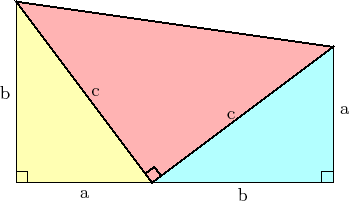
\includegraphics{./inputs/RightTriangle}
\end{center}
\end{Verbatim}
\begin{center}
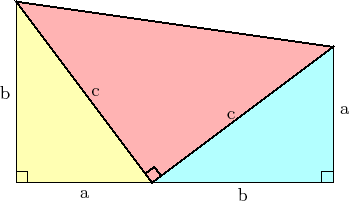
\includegraphics{./inputs/RightTriangle}
\end{center}
\subsubsection{Other details.}
The \verb+pst*+ packages should be loaded the latest on the preamble. Specifically \emph{after} other graphics packages like \verb+graphicx.sty+, \verb+color.sty+ which seem to break \verb+\psgrid+ and other commands.
\subsubsection*{xypic}

To be written.

\subsubsection*{MetaPost}
MetaPost is a graphics package designed for TeX (and LaTeX). It is operated by describing the desired diagrams in a relatively simple programming language. More information can be found at: \htmladdnormallink{http://cm.bell-labs.com/who/hobby/MetaPost.html}{http://cm.bell-labs.com/who/hobby/MetaPost.html}

Here is a discussion of the aspects of MetaPost that may help you decide if you want to use it for your diagrams.

\textbf{Advantages}:
\begin{itemize}
\item
Easier to learn and use for creating technical drawings than general purpose programming languages. Also, the language is more high-level than PostScript. The language has support for conditional execution, loops, variables, functions, subroutines, and recursion. Basic graphics primitives such as B\'ezier curves, lines, circles, and affine transformations are directly supported in the language.
\item
Most computations needed for the drawing can be left to the computer. You just program in MetaPost the equations to be solved, with whatever given inputs.
\item
Much better than most GUI drawing packages when your diagram has mathematical
constraints. Diagrams can be made \emph{precise} (which may well be impossible when drawing them in a mouse-based program). And very importantly, your diagrams can be \emph{parameterized},
so if you decide to change some angle in a figure --- which may often in turn affect other parts of the figure --- you can just change one number in the diagram source code --- no need to redraw the whole diagram.
\item
It is possible to quickly reuse parts of figures, provided the source code for the diagram has been written well enough.
\item
There are abundant well-written tutorials and manuals for MetaPost.
\item
Typesetting formulae in the diagrams is easy: Labels are written directly in TeX
or LaTeX.
\item
Clear text MetaPost source code can be created with any text editor.
The output is encapsulated PostScript.
\end{itemize}

\textbf{Disadvantages}:
\begin{itemize}
\item
Obviously, it is not point-and-click. There is some effort (about a few hours for this writer) to learn enough of the language to produce useful diagrams. The command-line interface to MetaPost is also not very well-designed, compared to other CLI programs.
\item
The programming language, because it is based on macro expansion, has more quirks and more cryptic error messages than some scripting languages, e.g. Python. No way around it.
\item
You need a working TeX system on your computer in order to preview diagrams
and to create the PostScript output for PlanetMath entries. (MetaPost comes installed with almost all TeX distributions.)
\item
There seem to be few libraries for artistic effects or more advanced graphics routines (e.g. 3D shading). That is because the MetaPost language is quick-and-dirty and not much suited for large libraries of this type. If you need these effects, you may have to code them yourself. (This author has written routines for displaying 3D objects in perspective.)
\item
As MetaPost uses fixed-point arithmetic, it is not suited for computing or plotting complicated transcendental functions. You probably would want to use some other package for these purposes. (However, MetaPost does have the trigonometric and exponential functions built in.)
\end{itemize}

\subsubsection*{gnuplot}

The gnuplot package (see \htmladdnormallink{http://www.gnuplot.info}{http://www.gnuplot.info}) can be used to produce graphs of functions and parameterized curves in Cartesian coordinates and polar coordinates. It can also do 3D surface plots.

\textbf{Advantages}:
\begin{itemize}
\item
Easy to get started and use.
\item
Has an interactive graphics interface for plotting, for both Windows and Unix-like systems.
\item
Has detailed reference documentation (but less on the tutorials).
\item
Source files are plain text files.
\item
Can typeset mathematical formulae in LaTeX.
\item
Functions are defined by expressions which can use the library of basic and special mathematical functions that comes with gnuplot itself. However, you cannot do general computations or programming in gnuplot.
\end{itemize}

\textbf{Disadvantages}:
\begin{itemize}
\item
The default options are quite ugly. You have to fiddle around a bit to get your plots to look right.
\item
But sometimes even that does not work. The formatting controls of gnuplot are fairly limited. In that case, you have no recourse but to use another tool.
\end{itemize}

\subsubsection*{PyX}

PyX (see \htmladdnormallink{http://pyx.sourceforge.net}{http://pyx.sourceforge.net}) is a software package, for the Python programming language, to produce mathematical graphics.

\textbf{Advantages}:
\begin{itemize}
\item
Gives access to most features of PostScript in an object-oriented language, at a level comparable to MetaPost.
\item
The mathematical graphics can be parameterized (using the expressiveness of the Python language).
\item
Powerful facilities for doing x-y graphs of functions. Almost every aspect of the plot --- color, positioning, tick marks, etc. --- can be adjusted by setting parameters. And for even more advanced usage (such as coloring in an area under the graph), you can roll your own Python code to do so.
\item
Can typeset mathematical formulae in LaTeX.
\item
Source files are Python programs.
\end{itemize}

\textbf{Disadvantages}:
\begin{itemize}
\item
Being based on a general-purpose programming language, when writing PyX graphs, there may be a lot of set-up and syntax that is irrelevant to the task at hand.
\item
You have to know the Python language fairly well to use this tool effectively.
\item
The documentation is terrible: it is mostly too terse for the beginner, and it assumes you know Python. However, there are an abundance of impressive examples on display at the PyX Web site that you can copy.
\item
Only the x-y graph facilities are well-developed. You have to roll your own routines for doing polar, parametric or 3D plots. Actually, for the task of plotting functions, rather than drawing vector-based graphics, matplotlib (see below) is probably the better way to go.
\item
The interface is not point-and-click.
\item
You need to have Python and PyX installed on your computer to be able to get the output.
\end{itemize}

\subsubsection*{matplotlib}

The software package matplotlib runs on top of Python and the SciPy package for it, for producing function graphs. Its programming interface is similar, but not identical, to that of the proprietary software MatLab.

\textbf{Advantages}:
\begin{itemize}
\item
Very good integration with the SciPy package for Python which provides advanced numerical computing facilities. You can, for example, program a finite-difference PDE solver and graphically plot the results all in one Python program.
\item
Easy to pick up if you ever used MatLab before. There is a good manual and good examples provided (but are unfortunately incomplete).
\item
There is a quick-and-dirty programming interface available, as well as an object-oriented interface in case you need it.
\item
Can be used interactively.
\item
Can typeset mathematical formulae in LaTeX.
\item
Source files are Python programs.
\end{itemize}

\textbf{Disadvantages}:
\begin{itemize}
\item
It is somewhat slow (at least when starting up the program).
\item
The installation of this and dependent packages is a little involved. If you are not into scientific computing and are only interested in doing a few simple plots of functions, matplotlib might be overkill for you.
\item
You need to have Python and PyX installed on your computer to be able to get the output.
\end{itemize}

\subsection*{Converting from other formats.} \label{gfxformats}



%%%%%%%%%%%%%%%%%%%%%%%%%%%%%%%%%%%%%%%%%%%%%%%%%%%%%%%%%%%%%%%%%%%%%%%%%%%%%%%%%%%%%%%
\chapter{Website documentation}

\abstract{This based on the list of existing site docs,
  which are available in their legacy format at
  \url{http://planetmath.org/?op=sitedoc}, and which were
  written by bbukh, mathwizard, akrowne, drini, PrimeFan,
  rm50, rspuzio, and CWoo, et al.}


\section{PlanetMath/Noosphere Scoring}
Why the heck do we have scoring on PlanetMath? Granted that PlanetMath is for ``serious'' content --- not video games. This is true, but there are still instances where it is desirable to have some approximate idea of how much
``value'' a user has contributed to the system. We developed scoring to be this ``value metric''. The first thing one can do with scores is simply to make them visible, at which point they can serve as an indicator of ``reputation''. This helps to direct beginners to experts, and helps experts identify each other to communicate at a common level. Another use for visible scores are to encourage competition. While this is probably not necessary, within communities like PlanetMath, it can't hurt.

In addition, there are situations where it'd help if the system itself had some rough idea of how ``valuable'' a user is. For example, the PlanetMath.org non-profit organization uses it as a criterion for membership --- acquiring a certain number of points serves as an indication that a particular person has added enough value and shown a level of commitment to be worthy of a say in the governance of the project.  

\subsection*{Scoring Breakdown}

Table \ref{tab:scoring} shows the current scoring chart as used on PlanetMath.

\begin{table}[h]
\caption{Scoring chart for PlanetMath}\label{tab:scoring}
\begin{center}
\begin{tabular}{|l|r|}
\hline
Action&Score Change\\
\hline
add a paper &+50 \\
\hline
add an exposition &+75 \\
\hline
add to encyclopedia &+100 \\
\hline
add a book &+100 \\
\hline
vote (in a poll) &+1 \\
\hline
post a message &+1 \\
\hline
accepted correction (erratum) &+30 \\
\hline
accepted correction (addendum) &+20 \\
\hline
accepted correction (meta) &+10 \\
\hline
revise an object &+5 \\
\hline
minor edit (for admins) &+5 \\
\hline
orphan/transfer an object &-(1/2)(score) \\
\hline
adopt an object &+(1/2)(score) \\
\hline
delete an object &-(score) \\
\hline
\end{tabular}
\end{center}
\end{table}

Wherever we've said ``score'', fill in the associated score from creating that particular type of object.


\subsection*{Conclusion}

These scores may not be what you'd pick. They are indeed somewhat arbitrary, and reflect the ideas of what we'd most like to encourage as content develops in PlanetMath. For this reason they may change over time.

There is a similar problem in everyday life that is analagous to our problem of how to configure scoring, which is at the core the problem of representing as closely as possible the amount of ``value'' that is created. The analogous problem is how much money should be minted to account for the amount of wealth that is created by a group of people living under a government. The government must try to estimate this added wealth as closely as possible, or risk major economic consequences. Here, the consequences are less dire, but to make the points (the ``coinage'') as useful as possible, we need to try to closely estimate the value (``wealth'') added to the system.

This analogy illustrates how this problem has no perfect solution, due to the subjectivity inherent in value. However, we have tried to come up with something functional. It is possible that we'll decide the way the scores are balanced does not work well, and end up changing them. If this happens, we'll post system news about it.

Suggestions are welcome as always!


\section{PlanetMath Automatic Reference Linking}

\subsection*{Motivation}
The PlanetMath encyclopedia is a ``semantic network'' of sorts. It is a set of concepts (entries in the encyclopedia) whose meanings depend, not only on the content of the entries, but on the position in the network (the connections to other entries.) This is of course the case because known mathematics represents one big semantic network. It is possible to understand portions of it that are only ``linked'' to each other and derive meanings from each other, but overall the entire ``network'' is connected and one must be able to move throughout the network to understand any given ``node'' (concept).

Because mathematics is like this, it is supremely important that users of PlanetMath are able to jump to requisite concepts in the network in order to understand the current one, all the way down to the concepts that are so simple they are evident to the intuition. However, there are so many of these connections that is is too much to ask for authors of entries to do the linking themselves. Not only is it too much work, but the authors just may not be aware of which requisite concepts are already defined on PlanetMath.

To solve this problem, PlanetMath implements automatic reference linking between entries in the encyclopedia. In essence, when an entry is ``rendered'' for display, the text is broken down and scanned for words that invoke entries that have been defined already. These words are then turned into hyperlinks. Doing this automatically almost completely frees the author from having to think about links, however, it is not completely infallible. Because of this, the user can ultimately override the automatic linking, or create their own original linking (see User Linking Controls.)

\subsection*{Behavior}
Linking is done, roughly, from instances of encyclopedia entry titles appearing in other entries, to those entries themselves. If there is an entry called ``widget'' in the encyclopedia, and I create a new entry ``thingamagig'' that contains the word ``widget'', ``widget'' in ``thingamagig'' will be turned into a hyperlink which leads to the ``widget'' entry.

There are more nuances to the behavior, however. What if I mention the phrase ``green widget'' in my ``thingamagig'' entry, and there is not only a ``widget'' entry, but a ``green widget'' entry? Well, in this case, the automatic linking is smart enough to link to ``green widget''. In general, the longest match at a given location in entry text wins, and shorter matches occurring ``within'' larger matches are ignored.

So, for example, say we have entries ``large green widget'', ``widget'', and ``large green''. If we mention ``large green widget'' in a new entry, all 3 words will become one hyperlink to the ``large green widget'' object, despite the fact that there are two matches starting at word ``large'', and the match to ``widget'' alone occurs at a different location, but is still within the set of words matched for a larger title.

Synonyms must be handled as well (synonyms are multiple titles for the same entry or concept.) Within the text of an object that has synonyms, all mentions of the object's title or synonym are escaped from linking. An example will illustrate why this makes sense. Say, in the ``large green widget'' entry, we mention the entire term ``large green widget'' (indeed, repeating the concept being defined is overwhelmingly common.) Since we expect these entire 3 words to define a single concept, but that concept is the current entry, we don't want them to be hyperlinked to ``large green widget'', ``large green'', ``green widget'', or ``widget'', ad nauseum. One might point out that the smaller titles may be requisite concepts, and one would be right in saying this. However, it happens that the natural tendency is for the author of an entry to think of all occurrences of the title or synonym in his entry as one concept, which results in explicitly mentioning requisite concepts. For example, invocations of ``green widget'' in ``large green widget'' that are not preceded by ``large'' will link to ``green widget'' as usual.

PlanetMath also performs a couple of ``morphological'' transformations on titles in order to ensure they are linked to. The first, and most important transformation, has the effect of invariance of pluralization. For example, creating an entry that says ``green widgets'' will link to the ``green widget'' entry. The second invariance is due to possessiveness. If there is a ``Green's theorem'' entry, mentioning ``the Green theorem'' in another entry will result in ``Green theorem'' being linked to the ``Green's theorem'' entry. This also works in reverse, if the entry was called ``Green theorem'' and you mentioned ``Green's theorem'', the linking would still take place.

Another morphological invariance concerns international characters. Plain Roman character versions of a title which contains western European characters will still be ``matched'' by the linking system. For example, ``Groebner'' will link to an entry entitled ``Gr\"obner.'' A TeX trigraph version like ``Gro\"bner'' will link properly as well.

The final transformation has the effect of invariance under title style. Titles can be phrased as index entries, containing a comma (like ``Mersenne, Marin'' for a proper name) or normally, like ``Green's theorem''. Users are encouraged to use index-style titles where appropriate, so that entries appear alphabetically in the encyclopedia where they'd be expected to appear. However, index-style titles could present a problem to the automatic reference linking if they were not handled; when mentioning Mersenne primes, nobody calls the inventor ``Mersenne, Marin''. Instead we'd say ``Father Marin Mersenne''. PlanetMath automatically takes care of this, so ``Marin Mersenne'' would link to ``Mersenne, Marin''.

There is one other important facet of behavior; linking is only done on the first occurrence of a concept. Why? Well, there is really no reason to make a link to every mention of ``widget'' if we have repeated it multiple times in an entry. We can assume our entry is read linearly, in which case the user will naturally follow hyperlinks immediately when they see a concept they dont understand. Once they come back to our entry, they understand the concept, so they don't need the hyperlink anymore. While we can't remove the link they just followed, we can avoid linking the rest of the occurrences of ``widget''. This also results in a much cleaner appearance, as links tend to make text look cluttered.

\subsection*{Behind-The-Scenes}
The link processing system is written in Perl, like the rest of PlanetMath. It is the single most complicated portion of the system. However, a decent explanation of how it works can be made without going into messy details (and they do abound).

The cross referencing engine starts by pulling out math environments and other portions of text that need to be escaped. These portions are replaced by single tokens, which are unique. The engine then first breaks the text of an entry into a single words/tokens array. This array form makes it easy to associate a particular word with a unique integer position.

All titles and synonyms in the encyclopedia are kept in a hash index structure. This structure contains at the top level only words that occur as first words of some title. Following these words leads to a list of entries that have titles starting with that particular word. This list is kept sorted in descending order of length, which allows the longest match to be chosen first, simply by early-out.

The now tokenized text of the entry is then iterated through. Checking to see if a word should be the start of a link is an $O(1)$ operation, thanks to the hash structure just described. If a word indeed matches the start of a title, the following words are checked to see if they match the longest title starting with that word. If this fails, the next longest title is checked, and so on. When a matching title is found, it is submitted to a subroutine for inclusion in the match array.

The match array is actually a hash of positions -- a match is first stored by the position where it matches within the entry text. When a candidate match is found, the match subroutine checks to make sure that no other entry already in the match array contains the position of the new match. It doesn't have to worry about checking to see if there is a longer match at the same position, because we already have guaranteed this by sorting titles by descending order of length.

After the match array is built, the engine iterates through it and replaces matching words with hyperlinks. The engine keeps track of when it makes a link to a particular entry, so that if it runs into another mention of this entry, a link is not made. Links are also kept in an array and returned to the calling PlanetMath code, so they can be displayed separately.

Finally, the linked text array is recombined with the removed tokens, and returned as a single text string. This final string is more or less what is sent to your web browser.

\subsection*{Asymptotic Complexity of the Algorithm}
If $n$ is the number of titles (and synonyms) in the encyclopedia, and $m$ is the number of words (minus escaped portions) in a new entry, it only ``costs'' $O(m)$ to process the new entry due to the above architecture! Notice how $n$ is not involved at all. This means that automatic reference linking is completely scaleable; as PlanetMath grows ($n$ increases), linking will not get any slower.



\section{Controlling Linking}
\subsection*{Introduction}

Noosphere's automatic linking system handles most inter-entry linking instances properly. However, a small fraction of the time, it does not have enough information based on concept label metadata (titles, synonyms, defines) and classification metadata to resolve ambiguous links. In these cases, something extra must be done to correct linking.

There are two families of methods to accomplish this. The first involves improving the metadata, beyond concept labels and classification. We introduce \emph{linking policy} metadata to accomplish this.

The second family of methods involves pseudo-\LaTeX{} commands to steer the linking. We call this the \emph{in-situ} method.

In-situ controls should be considered a last resort, as it is much more elegant and labor-effective to separate link controls from the text. For example, consider a situation where someone points out a problem with a link in your entry, entry $A$. The errant link is due to a term defined in entry $B$. This problem could be fixed if the author of $B$ improved its linking policy, or if you used an in-situ link steering command in $A$. However, assume that the same linking problem is also present in 100 other entries, all of which link to $B$. Rather than fixing the 100 entries with in-situ commands, it makes much more sense for the author of $B$ to modify its linking policy once, solving all 100 errant link instances.

The two families of methods are described below.

\subsection*{Linking Policy}

The linking policy of an entry is a text field containing a set of directives, one per line. The currently-supported directives are described below.

\subsection{Link Priority}

This directive has the following syntax:

\begin{verbatim}
 priority <N> [LABEL]
\end{verbatim}

 where \verb=<N>= is a number and \verb=[LABEL]= is an optional concept label defined by the entry. The default priority is 100, and integer values from 0 to 32767 are accepted. Smaller numbers mean higher priority. Examples are:

\begin{verbatim}
 priority 10 normal
 priority 200 "mapping function"
\end{verbatim}

 This directive is used as a tie-breaker when classification directives and category-based link steering fail to find a unique destination. Setting the priority higher than normal (closer to zero) results in an entry (or concept) being linked to ``by default''. Setting it lower (above 100) would result in the entry or concept being linked to automatically only when the categorization of the other entry overlaps.

\subsection*{In-Situ Link Controls}

The in-situ methods involve pseudo-\LaTeX{} commands you can put in your entry to steer linking. As mentioned before, they should be considered a last resort, with proper concept labels, classification, and linking policy as the first lines of defense.

\subsubsection*{Link Suppression}

Sometimes it makes sense to block linking entirely for a portion of an entry, rather than simply steering a link to a different target. Below are a number of commands to do this:

\begin{description}
\item [\texttt{\textbackslash{}PMlinkescapetext}]
 Usage: \texttt{\textbackslash{}PMlinkescapetext\{text\}} or \texttt{\{\textbackslash{}PMlinkescape text\}}\\
 This will result in ``text'' appearing rendered verbatim with no reference link processing applied to it. Note that these only act upon the single body of ``text'' given.
\item[\texttt{\textbackslash{}PMlinkescapeword}]
 Usage: \texttt{\textbackslash{}PMlinkescapeword\{word\}}\\
This will result in ``word'' being exempt from reference link processing anywhere it occurs, separated from other text by blanks, in the object. This tag can appear anywhere inside the text of the article (including at the end of the object, but \emph{not inside the preamble}). Note that this tag produces no output.
\item[\texttt{\textbackslash{}PMlinkescapephrase}]
 Usage: \texttt{\textbackslash{}PMlinkescapephrase\{phrase\}}\\
 Results in the series of words ``phrase'' being exempt from reference link processing anywhere they occur in the object. In fact, this tag is currently implemented the same as \texttt{\textbackslash{}PMlinkescapeword}. However, it is conceivable that words and phrases may be treated differently at some point, so one should keep this in mind when deciding which command to use. Note that this tag produces no output.
\end{description}

\emph{Warning:} If you put \texttt{\textbackslash{}PMlinkescapeword} in your preamble, it may or may not work, and it may or may not cause random breakage of other things in your document. Do not do this!

As an example, suppose I have an entry that looks like this:
\begin{quote}
\begin{verbatim}
Fix a prime $p$.
Then $p$ is odd if and only if $p\neq 2$.
\end{verbatim}
\end{quote}

As it stands, the word ``fix'' will be autolinked to an entry on fixed points. This is not appropriate here. So we have two choices:
\begin{quote}
\begin{verbatim}
\PMlinkescapetext{Fix} a prime $p$.
Then $p$ is odd if and only if $p\neq 2$.
\end{verbatim}
\end{quote}
or
\begin{quote}
\begin{verbatim}
\PMlinkescapeword{Fix}
\PMlinkescapeword{fix}
Fix a prime $p$.
Then $p$ is odd if and only if $p\neq 2$.
\end{verbatim}
\end{quote}

In the first case, if ``fix'' occurs again in the document, it will be autolinked, even though the first occurrence is not. This is appropriate if the second occurrence is actually using it in the technical sense. In the second case, the word ``fix'' is never autolinked; if you do use it in the technical sense, you should use one of the commands below to link it.

Both capitalizations are included in the entry above because the autolink suppression is very simple: it only suppresses links from identical text. So in order to prevent autolinking on ``fix'' as well as ``Fix'', we have to explicitly specify both.

\subsubsection*{Link Steering}

Using classification and linking policy, automatic linking can usually pick the correct destination for a link when there are multiple possibilities. However, when it fails, one might have to use a link steering command instead.

\begin{description}
\item[\texttt{\textbackslash{}PMlinkid}]
 Usage: \texttt{\textbackslash{}PMlinkid\{anchor\}\{id\}}\\
This links text ``anchor'' to the PlanetMath encyclopedia object with id ``id''. You can find out an object's id when you view it. Produces a single instance of ``anchor'' hyperlinked where the command is issued.
\item[\texttt{\textbackslash{}PMlinkname}]
 Usage: \texttt{\textbackslash{}PMlinkname\{anchor\}\{name\}}\\
 This links ``anchor'' text to the PlanetMath encyclopedia object with name ``name''. Note that name is a PlanetMath canonical name. You can also find this out by viewing the object. Produces a single instance of ``anchor'' hyperlinked where the command is issued.
\end{description}

\subsubsection*{Manual Linking}

There are instances where entirely ad hoc links are desired, such as to an external object on the web, or to a file box. For these instances, a manual linking pseudo-\LaTeX{} command is necessary. These commands are described below:

\begin{description}
\item[\texttt{\textbackslash{}PMlinkexternal}]
 Usage: \texttt{\textbackslash{}PMlinkexternal\{anchor\}\{url\}}\\
 This allows you link to any arbitrary URL on the web within your object. ``anchor'' is the text which will appear in your rendered object. URL is the address you want to point to. This corresponds to \texttt{<a href="url">anchor</a>}.
\item[\texttt{\textbackslash{}PMlinktofile}]
 Usage: \texttt{\textbackslash{}PMlinktofile\{anchor\}\{filename\}}\\
 This links ``anchor'' text to ``filename'' in the object's filebox. One caveat: when previewing a new object, the URL generated for this command will not work.
\end{description}

\subsubsection*{Notes}
Since there is no sophisticated parsing of the pseudo-\LaTeX{} commands, you can't put anything ``fancy'' inside the brackets for them. That is, plain text only. You cannot do something like \texttt{\textbackslash{}PMlinkescapetext\{\textbackslash{}emph\{function\}\}}, you'd have to do \texttt{\textbackslash{}emph\{\textbackslash{}PMlinkescapetext\{function\}\}}.

These commands are implemented entirely in the code for PlanetMath, during the preprocessing that happens before the \LaTeX{} content is sent to the rendering back-end. They were modeled after \LaTeX{} commands in order to keep the overall content representation paradigm consistent.

There is a package \texttt{\htmladdnormallink{pmath.sty}{http://aux.planetmath.org/files/objects/4630/pmath.sty}}
that allows one to process the above commands if either of the following packages is used: \texttt{hyperref}, \texttt{html}, \texttt{url}. If no such package is used, then no hyperlinks are created.

%It is possible at some point a PlanetMath LaTeX package will be created which %will allow one to usefully render a PlanetMath encyclopedia object in other %contexts. That is, the package would remove the \textbackslash{}PM tags, and %leave %the anchor texts. Or it could be really smart and translate all of the %internal %links to external links that point to the proper location in %PlanetMath. Nothing like this exists yet, however.

All links are implemented using the actual \LaTeX{} \texttt{html} package, with the \texttt{\textbackslash{}htmladdnormallink} command.


\section{Noosphere's Authority Model}
\subsection*{Overview}
An important aspect of a collaborative content-creation system is the authority model. The model should define who has permissions to add content, who can remove things already created, who can modify them, and how these facets of authority evolve with time.

This document will explain what Noosphere's authority system is, how it works, and give some justification for this particular design.

\subsection*{Ownership}
The foundation of Noosphere's authority model is that of the object owner. At it's simplest level, this system is what you might expect: the person who creates an object becomes its owner, and basically has complete control over what kind of changes are made to the object. They are the gatekeeper for all changes to the object, and their judgement is assumed to be reasonable.

The motivation for this system was to appeal to the natural instinct of valuing and perfecting that which one has created, especially when this work is on display for a large community. When a single name is associated with a work, the quality of that work becomes a statement about its creator. Hence, the ownership model encourages quality work on sites running Noosphere.

However, if this were the end of the story, such sites would be in pretty poor shape. The problem is that we can never assume that an object is ``complete,'' and experience shows us that this is a reasonable assumption. This fact clashes with the observation that people in any (online) community come and go, their attention waxes and wanes, available free time varies considerably, and interest can in some cases quickly fade.

Not only may a user create an object and never return to maintain it, but it is simply too much to ask that a user maintain their contribution to the site in perpetuity. A solution is needed that strikes a compromise between singular ownership and community involvement in order to account for a shifting user base (one can never step in the same river twice, similarly, a site running Noosphere is never the same between each visit.)

\subsection*{The Adoption System}
One solution to this problem is to follow the Wiki model and simply allow anyone to modify objects, completely overturning the ownership model. Clearly this solution brings to an end the system of ``the owner,'' and incentives to at least attempt to take full responsibility for an entry are somewhat diminished.

In addition, this model is somewhat inappropriate for mathematical and scientific content. Requiring a correction to be filed in order to suggest changes creates a dialog around these proposed changes. This is good because there typically is a ``right'' answer in these fields, and it may not be obvious to the casual observer who might just happen by and think they see something wrong.

Though the ability to roll back changes in Wiki can ``simulate'' the rejection of corrections in Noosphere, the dialog surrounding corrections is more appropriately formalize, preserved and packaged in Noosphere. For these reasons and others, it is widely believed that this is not a good authority model for sites developing mathematical or scientific content.

The best compromise then seems to be allowing some form of shifting ownership, and this is in place currently in the form of the orphaning and adoption system.

Under this system, objects with long-lived pending corrections become targets for adoption first, and then later orphaning. At 6 weeks, any other user can ``adopt'' one of these objects from the ``orphanage,'' at which point they become owner of the object. At 8 weeks of a pending correction, ownership of an object is completely removed, and the object is fully ``orphaned.''

Of course, before either of these stages is reached, the owner of the entry is notified of the situation. Beginning at 2 weeks of a pending correction and continuing every week until orphaning, an owner is sent e-mail nags informing them of the situation.

This system has been observed to work very well so far. It allows motivated and active users to take neglected objects ``under their wing,'' and the same incentives which come from singular ownership can continue.

\subsection*{The ACL System}
Strictly speaking, the ownership system, along with adoption, is ``complete'' in that it succeeds in providing for continuity of maintenance. However, it was realized after a while that things could be nicer. What seemed to be missing is the ability to make the decision to ``share'' responsibility for an entry between two or more people, effectively making the creator of an object a group-like entity. The singular owner system is nice as a starting point, but in the real world, multiple authors are common.

This is somewhat different again from the Wiki model in that the author group still should be restricted. Thinking of the group of authors as a Noosphere ``user'' which acts as the owner of an object is a good approximation.

This system has been implemented with ACLs, or \emph{Access Control Lists}. The starting point for any new object is to have one owner who is ``superuser'' with regards to that object, but this person can, if they choose, use ACLs to define other users or groups of system users who should also have edit access to the object.

The access rules in Noosphere are simple. A single rule specification consists of read, write, and ACL flags, and a subject (which can be a user or a group). Or, instead of a subject, the rule can be ``default'' in which case it is applied to users for whom no other matching rule can be found (the user isn't explicitly mentioned in a rule, or isn't in a group that is mentioned). The ``read'' and ``write'' flags are fairly self-explanatory. The ``ACL'' flag simply determines whether or not the subject can also define ACL rules for the object. Granting a subject ``ACL'' permission is akin to making this subject an ``admin'' or ``editor'' (rather than author) of the object.

These rules allow Noosphere to subsume the Wiki authority model where this is desired, since an owner can include a default access rule to make their objects world-writeable. But orphaning and adoption still applies as before, so this universal authoring status must be maintained by actual participation and upkeep.

More importantly though is the added flexibility the ACL system affords the ownership model, generalizing the concept of ``owner'' to a group. It is anticipated that this will be commonly needed, as it is possible to begin an entry from one approach and with one facet of expertise, but later discover that there are many other facts to the concept which it would do better to have other ``experts'' write about. In this situation, changing ownership seems less reasonable than simply expanding the set of authors, to properly give all parties credit.

\subsection*{Conclusion}
Of course the above system is very unique and experimental, and time will tell how well it all works out. The authority system has always been evolving in Noosphere and it is not certain that it is finished evolving. Suggestions and criticisms are welcome as always. The authority system must, after all, conform to the way people do things, so we'd love to hear from you.





\chapter{Nonprofit documentation/transparency}

\abstract{This is based on a list created by Ray; see
  below. There may be things to add to this list from
  Joe's "transparency-enhancing" project from earlier in
  2009, see for example
  \url{http://aux.planetmath.org/doc/sponsor.html}.}

\section{A half-page executive summary}

PlanetMath.org is a 501(c)3 tax-exempt non-profit, incorporated in the state of
Virginia.

Aaron Krowne got the website off the ground in 2001 and completed his
"PlanetMath thesis" in 2003 at Virginia Tech. PlanetMath.org, Ltd. was
incorporated the same year, and granted tax exempt status 2004. In 2006, we
became part of the Google Summer of Code program, which funded a series of
enhancements to PlanetMath's linking system, and a new rating and reputation
system, among other projects. In recent years, we contracted with the IMS and
Berkeley CPAM to make other improvements to Noosphere.

Our programming team is currently finishing up a set of enhancements to the
editorial and moderation facilities in Noosphere, under contract with Springer.
We are also helping build the Bibliographic Knowledge Network, a project funded
by an NSF and managed by Jim Pitman at UC-Berkeley.

A lot of the things we want to work on, both in software development and
community projects, will require both increased funding and better
organization. As we go forward, the way our content is licensed, the way we
facilitate editorial work, and even the centrality of the encyclopedia on
PlanetMath will all be questioned, and possibly revised. Our organization will
need an active staff if we are going to make effective changes in these or
other areas. For the immediate future, expect to see us focused on becoming a
better-functioning organization.


\section{Vision, mission, and goals}
\input{VissionMissionGoals.tex}

\section{Contact information}
Physical mail: 

\indent PlanetMath c/o Bonnie Rabichow \\
\indent 4336 Birchlake Ct. \\
\indent Alexandria, VA 22309 \\
\indent USA

\noindent Email:

\indent \url{feedback@planetmath.org}

\noindent PlanetMath's secretary, by phone:

\indent +1-505-INKY-PEN


\section{Current personnel (board, administrators, staff, etc.)}

The board of directors is:
\begin{itemize}
\item Aaron Krowne (PlanetMath Founder and President)
\item Joseph Corneli
\item Roger Lipsett
\item Raymond Puzio
\item Chi Woo
\end{itemize}

Board members are elected by voting members of PlanetMath, and serve for one
year. The board is responsible for deciding how PlanetMath's budget is spent,
including for hiring and overseeing staff or contractors; and for deciding and
maintaining site policies, including the appointment of site administrators.
The board is not compensated for this work, although board members can and do
at times serve as independent contractors with the organization. Our quarterly
board meetings that are open to the public; the dates of these meetings are
announced as news items on the website and on our mailing lists.

The mathematical content you find on the website is developed and maintained by
volunteers in our user community. Site users as a whole are responsible for
producing the content found on PlanetMath, and for reviewing and critiquing the
content other users have posted. A handful of users have special administrative
privileges. Site administrators can delete highly objectionable content and
suspend or remove a given user's posting privileges. Site administrators are
not compensated for their work.

Board members, administrators, and other active community members can be
reached through our mailing lists or the PlanetMath forums. The specific
policies of PlanetMath are published at:
\url{http://planetx.cc.vt.edu/AsteroidMeta/PlanetMath}.
Additional informal policy items of interest to site users are
available at: \url{http://planetmath.org/docs/}.


\section{Membership and Subscriptions}

We have just begun a subscription memberships system, through which you can
financially support the PlanetMath organization and community on an ongoing
basis (click the previous link to enter the system).

There are perks to supporting financially in this manner:
\begin{itemize}
\item voting rights -- for site administration, community development, and
      governance issues.
\item being listed on our "great wall" of donors
\item receiving the PlanetMath quarterly newsletter.
\item news, announcements, and other updates concerning the community and the
      nonprofit.
\item potential "goodies" in the future, as we can afford them (e.g., the
      encyclopedia in print, t-shirts, etc.)
\item meeting/symposium discounts (anticpiated).
\item of course, satisfaction in helping materially support PlanetMath!
\end{itemize}
We strongly encourage friends of PlanetMath who believe in free knowledge (in
all senses) for mathematics (and beyond) to become a member, at least at the
minimum level (\$20/yr). A steady revenue stream holds the promise of a much
greater ability of the PlanetMath community to sustain, grow, develop and
attain much greater impact.
One time donations can also be performed via PayPal (which also accepts credit)
through the above system, or via one of the methods described below.


\section{Donating to PlanetMath}

PlanetMath needs your help! While we have been a great success in producing
mathematical content through the volunteer work of the community, our resources
have fallen distressingly short of needs in terms of delivery and development.

In specific, we'd like to hire people to various extents to:

\begin{itemize}
\item perform server administration
\item fix bugs and make small updates to the collaborative system (Noosphere)
\item undertake more extensive software development
\item manage the nonprofit org (maintenance, governance of the community,
      development, support-seeking)
\end{itemize}

Right now, as much as any of these things are done, they are done in what
little volunteer time a few people can spare and are therefore lacking greatly
in consistency and scale. Currently we pull in about \$5000/yr from ads and
donations; we figure we need about \$40,000/yr to really start hiring people (at
first, either a developer/admin or part time of each). Our near-term target for
public donations, however, is \$10,000/yr, and we are about a third of the way
there.

We need your help to improve quality of service of PlanetMath and continue to
help the software and community grow and evolve. We hope that, if you feel
PlanetMath is a great resource, you will consider one of the following forms of
assistance.

Note: PlanetMath is a US-based nonprofit corporation, "PlanetMath.org, Ltd.",
incorporated in Alexandria, Virginia. It is a 501(c)3 tax-exempt public
charity, so donations from US residents are tax-deductable!

Liquid cash is probably the best way to help us out, because we can turn it
into most anything else we need to improve the delivery and development of
PlanetMath. We are open to large-scale grants from nonprofit and government
organizations or private corporations, private and public sponsorship
arrangements, and private donations from individuals. Though we don't have a
formal monetary-base membership arrangement for the PlanetMath.org, Ltd.
corporation (for now), we suggest a standard yearly donation of \$20US-\$100US
for individuals who are able and use PlanetMath regularly or just want to
support the effort.

You can get money to us as follows:

\begin{itemize}
\item Use our PayPal "donate" button.
\item Send a check to:
      PlanetMath Donations
      C/O Bonnie Rabichow
      4336 Birchlake Ct.
      Alexandria, VA 22309
      USA

\item Get matching donations. Many employers will match donations made by their
      employees to registered tax-exempt public charities. This is a very easy
      way to increase the power of your donations. By how much? Before we were
      tax-exempt and employers couldn't match donations, a dollar donated was a
      dollar towards PlanetMath. Now, since you can write off your donation and
      get your employer will match it, every (approx.) 2/3 dollar is two
      dollars for PlanetMath. In other words, each real dollar you contribute
      is three for PlanetMath (given matching and standard tax assumptions)!
      Find out if your employer has a program like this, and give the handler
      your proof of contribution and our tax identification number 42-1605465
      when you make a donation.
\item Buy goodies from our CafePress Store.
      This also has the added benefit of spreading the word about PlanetMath to
      all who see your PlanetMath gear (however, keep in mind we only get a
      small slice of the sale price).
\item Grants or sponsorships - Please contact us at the email address at the
      bottom, or send a letter to the snail mail address above. You can also
      call us vox at 404-712-2810.
      We think that this type of support has the potential to enable more
      forward-thinking development of PlanetMath/Noosphere and collaborative
      digital libraries in general. If you are interested in funding research
      and development in this area, please get in touch with us.
\end{itemize}

Donations of facilities or hardware may be useful to us, depending on the
specifics of the situation. Small-scale hardware, such as spare, stand-alone
home or home-office computers, will probably not be useful to us. However, we
would eagerly consider grants of rack-mountable, mid- to large-scale
multiprocessing or clustering systems.

Volunteering your time and expertise is a great way to help out. We are looking
for people who can code and want to help fix bugs and optimize PlanetMath and
the Noosphere system (as well as to extend them). We chiefly use Perl at the
moment, but we can usually make use of good coders who don't work in that
language. We are also interested in ideas for improving PlanetMath's
architecture to make it more elegant, efficient, maintainable, extensible, and
scalable.

We encourage all prospective volunteers to join in the activities on our
planning and coordination wiki, AsteroidMeta. Here are the PlanetMath and
Noosphere sections.

Please send inquiries about any of the above methods of assistance to
feedback@planetmath.org. Volunteers should check out the collaboration wiki
mentioned immediately above. Thanks in advance! -- Aaron Krowne
President, PlanetMath.org, Ltd.


\section{Finances and budget}

\subsubsection*{Financial summary}
Historically our income has come from individual donations, Google ads, and
some cash support as part of the Google Summer of Code. In 2006, one of our
major contributors made use of the Microsoft matching donations program,
pushing our income to a record level (over \$10,000) that year.

\begin{table}
\begin{center}
\begin{tabular}{lllll}
{\bf Year} & {\bf Income} & {\bf Expenses} & {\bf Net} \\ 
2005 & 2836.01 & 1266.54 & 1569.47 \\ 
2006 & 11850.21 & 7486.47 &  4363.74 \\
2007 & 4391.63 &  7263.42 & -2871.79 \\ 
2008 & 9694.00 &  3961.14 &  5732.86 \\
\end{tabular}
\end{center}
\caption{Summary of Income and Expenditures}
\end{table}

\begin{table}
\begin{center}
\begin{tabular}{lll}
{\bf Year} & {\bf Income} & {\bf Expenses} \\
2005 & 25\% from ads & 90\% legal fees \\ 
2006 & 14\% from ads & 37\% for honoraria, 20\% for travel, 26\% subscription system \\
2007 & 40\% from ads &  41\% for contract labor, 37\% travel  \\ 
2008 & 11\% from ads &  38\% for contract labor, and 36\% travel \\
\end{tabular}
\end{center}
\caption{Income from ads; major expenditures}
\end{table}

\subsubsection{Projected Annual Budget}

Our goal is to raise \$50,000 this year. This is very close to the estimated
annual "true cost" of PlanetMath's operations. However, an annual budget of
\$50,000 would do more than just maintain the status quo. With this kind of
funding, our work would begin to thrive. In recent years, we've have money in
our bank account that we don't have a good way to disperse, i.e., we don't have
enough money to offer long-term contracts to skilled, motivated workers who
require a degree of stability in their employment. Although we have a volunteer
effort adding up to about 3/4 time of a staff person, this effort is spread out
over people who are not always available.

\begin{table}
\begin{center}
\begin{tabular}{ll}
\$15600 & non-profit administration, half-time position \\
\$15600 & systems administration, half-time position \\
\$15600 & software development, half-time position \\
\$1200  & a server that doesn't crash \\
\$2000  & travel reimbursements \\
\end{tabular}
\end{center}
\caption{Projected Budget}
\end{table}

Although a \$50,000 budget defines and fills the major spending areas, a
benefits package would help us attract first-rate personnel. Similarly, whether
we begin with an annual budget of \$50K or \$75K, salary increases over time will
be required if we're going to retain these individuals. Accordingly, we would
like to see budgetary growth of \$5K to \$10K per year.

\subsection*{True Costs of Operations}
Since 2006, Google Summer of Code has also sponsored a total of 9 internships
at PlanetMath, an in-kind contribution valued at up to \$45,000. We've also
received facilities support from Virginia Tech since our inception, at an
estimated value of \$100/mo. Direct funding for development of Noosphere from
the IMS, Berkeley CPAM, and Springer in 2006-2009 has come to approximately
\$16,000.

Thus, money or services worth \$64000 on the open market have been spent on
behalf of PlanetMath over the past three years. This comes to roughly \$21,333
dollars per year above our average yearly cash expenditures of \$6770 over the
same period of time.

However, the true cost of operating PlanetMath is considerably more than
\$28,103 per year. The volunteer contributions of time and effort from a wide
range of people make PlanetMath what it is. Assuming out of the group of
volunteers involved with overseeing the day-to-day operations of PlanetMath,
there have consistently been 3 persons contributing 10 hours a week that would
be valued at \$15/hr on the open market, site and non-profit management has
donated about \$23,400 per year.

This puts the true operating cost of PlanetMath as an organization at upwards
of \$51,503 per year.

Further information on PlanetMath finances are available
from our Treasurer, Bonnie Rabichow
(\url{bonsuerab@gmail.com}).

\subsection{The Societal Value of PlanetMath}

User scores are meant to give a relative estimate of the value different users
have contributed to PlanetMath. However, we can also use these scores to
estimate the total value of user contributions. Here are two such estimates
(using data from March 9, 2009):

\begin{table}
\begin{center}
\begin{tabular}{lll}
                                    & {\bf \$0.05 per point} & {\bf \$0.50 per point} \\
Value of a new article              & \$10             & \$100 \\
Highest scoring user's contribution & \$5,145          & \$51,449 \\
Top fifty user's contribution       & \$55,371         & \$553,714 \\
Top one hundred user's contribution & \$62,388         & \$623,884 \\
Approxmiate total user contribution & \$75,000         & \$750,000 \\
\end{tabular}
\end{center}
\caption{Estimated value of user contributions}
\end{table}

Regardless of which estimate is more accurate, the question of how much it
would cost to build the website is, by itself, not a particularly useful
estimate of the value of the site.

For one thing, since PlanetMath is built by volunteers, so we can assume that
each volunteer actually gets something valuable out of contributing, and
replacing their labor power on the open market would remove this "volunteer
surplus". The volunteer surplus is what people would pay to be a contributing
members of PlanetMath. Our suggested minimum membership donation is \$20/year,
although we waive that fee in the case of users who contribute sufficient
content. If we use this amount as our estimate of the average volunteer
surplus, then we'd expect one hundred active users to generate a surplus of
\$2000 per year.

Second, the fact that we get 12,000 to 20,000 web hits per day means that there
are many users who get value out of PlanetMath without contributing content. We
note that if one percent of PlanetMath visitors each day found their experience
worth \$1.25, their small monetary contributions would cover the real cost of
running the site. Similarly, our real costs would be covered if every single
page hit earned \$0.0125 for PlanetMath. If this billing rate per hit reflects
the real value of PlanetMath to non-contributing users, then over the past 5
years, we have delivered over a quarter of a million dollars worth of content
to the mathematical public.

This suggests that the value of PlanetMath in both capital
accumulation and services rendered to date is at least
\$335,000, and perhaps as much as a \$1 mil.

\subsection*{Towards a sustainable business model for PlanetMath}

Several categories of income sources could be drawn on to raise funds
sustainably. 

\subsubsection*{Donations From Community Members}
As noted above, if one percent of PlanetMath visitors each day found their
experience worth \$1.25, their small monetary contributions would cover the real
cost of running the site. Users should be made aware of this and encouraged to
provide \emph{small} donations when they find the site useful. Now that we have a
membership system, we should be doing membership drives and donation drives
more regularly, in particular, so that we can be understood. We need better
practices for running funddrives!

\subsubsection*{Switch from Advertising to Sponsorship}

As noted above, our real costs would be covered if every single page hit earned
\$0.0125 for PlanetMath. If we could make an arrangement with a corporate
sponsor willing to pay \$12.50 CPM or about \$150.00 per day, this would meet our
costs. Even something considerably lower than this would still be an
improvement over Google AdSense.

\subsubsection*{Rendering Services to Outside Entities}
Lately one of our biggest sources of productive income has been contract work
with other organizations (IMS, Berkeley CPAM, Springer) for improvements to our
open source software platform, Noosphere. With a stable staff, we will be in a
better position to be able to provide dedicated services to entities interested
in mathematics research, education, or publishing, or who are interested in
using our software.

\subsubsection*{Selling Copies of the Encyclopedia and Other Derived Works}
A stable staff, along with the roll-out of recent changes to the Noosphere
platform, will help us create a centralized editorial system whose role it
would be to certify certain articles from the PlanetMath encyclopedia for
inclusion in a print encyclopedia. Combining editorial improvements with
existing code that automates a significant portion of the technical editing
needs, we could produce new editions and supplements to our print encyclopedia
at regular intervals. The Encyclopedic Dictionary of Mathematics sells for
about \$100; a typical Springer graduate text sells for about \$50. Our ability
to turn the content of the web-based PlanetMath corpus into a variety of
derivative paper-based products is what stands between us and opening this new
revenue stream.

\subsubsection*{Running a Tutoring Service}
The idea of running a tutoring or question-answering service through PlanetMath
has been circulated many times over the past years. A stable staff and the
right partnerships would help us get such a service of the ground. Receiving
tutoring over the internet is not a new thing, but having the tutoring service
integrated with an open, well-indexed, electronic archive of past answers and
other mathematical content would make PlanetMath an attractive option for
students seeking help.


\section{Current Committees and Policies}
We used to have a ``Content Committee'', but it has since been dissolved.

%\section{Content Committee Charter}
%
\subsection*{Preamble}
This document serves as the charter for and supplementary operational details of the PlanetMath Content Committee, an official committee of the PlanetMath board.

This charted is not meant to lay out thorough procedures for accomplishing the goals of the committee; instead, part of the job of the committee will be, by experimenting, to understand and codify procedures that work in the context of the PlanetMath community, and formalize them later. This includes things such as what improvements would provide the most benefit as well as what kinds of inducements will work best to standardize the quality of PlanetMath submissions. This document, then, is meant to provide a basic operational framework and overall direction for the Content Committee.

The document may be amended at any time, at the recommendation of the Content Committee. The PlanetMath Board will once again be required to approve any such changes. Unless clearly marked as drafts of proposals or changes, all of the content of this document should be considered official operational policy.

\subsection*{Purpose}
The mission statement of the Content Committee is:

\begin{quote}
\textbf{The Content Committee will preserve and maintain the integrity and quality of the mathematical content and organization of PlanetMath.}
\end{quote}

To this end, the committee will engage in activities designed to improve the accessibility of information, improve the accessibility of the site to new members, improve the content, style, and correctness of individual entries, and ensure that other aspects of the site such as the request list are adequately maintained. In order to do this, the committee will need a substantial active membership, which will be recruited from active PlanetMath members.

\subsection*{Charter}
\subsection*{Organization}

The membership of the Content Committee will be determined by the Board of PlanetMath. When the board determines that additional member(s) is (are) required, the Content Committee will seek to recruit new members.

The Content Committee shall in general seek to find new members who are not already PlanetMath board members.

The Content Committee may set out procedures and policies regarding Content Committee recruitment and tenure. However, all new members and forcible Content Committee ejections must be approved by the Board.

\subsection*{Content Committee Documents}

In order to carry out PM content-related responsibilities/tasks, the PM CC may develop specific policy documents. Below are some examples of ``Content Committee related'' documents:

\begin{enumerate}
\item Standards of PM Content with respect to its Encyclopedia, Paper, Exposition, and Book Sections
\item Enforcement Rules with respect to PM Content (which does not include individual behaviors in the PM Forum)
\item Rules and Regulations regarding PM Request System and PM Orphanage
\item PM Point System
\end{enumerate}

Except on matters having to do with the suspension of a PM user or forcible removal of a Content Committee member, tasks spelled out by these documents may be executed completely within the discretion of the Content Committee.

\subsection*{Primary Content Committee Responsibilities}

Areas of work that are currently seen as important include (but may not be limited to) the following:

\begin{enumerate}
\item Developing/maintaining the standards for PlanetMath content
\item Improving individual PlanetMath entries in its Encyclopedia, Book, Paper, and Exposition)
\item Developing topic areas
\item Developing/improving site and user documentation
\item Managing the PlanetMath Request list and Unproved Theorems list
\item Improving categorization and other meta-attributes of entries.
\item Developing software recommendations for improved content authoring and editorial functions.
\end{enumerate}


\subsection*{Accountability and Documentation}
The Content Committee will provide the Board such information as it
demands to make decisions on Content Committee requests.


\subsection*{Detail}

\subsection*{New Membership Recruiting Procedure}

The procedure for adding members will be as follows:

\begin{enumerate}
\item The content committee will post a note on the PlanetMath forums asking for nominations, or for self-nominations. A nomination shall consist of an application per format specified by the Content Committee in the announcement.
\item A reminder post will be made one week later.
\item After two weeks, existing nominations will be collected and evaluated by the current content committee.
\item Names of successful candidates will be forwarded to the Board for final approval.
\end{enumerate}

\subsection*{Content Committee Responsibilities}

Some of the responsibilities mentioned above are described in more detailed below.

\paragraph{Standards for PlanetMath content}
The \texttt{\htmladdnormallink{PlanetMath Community Guidelines}{http://planetmath.org/?op=getobj&from=collab&id=137}} provides in Section 4 a preliminary discussion of standards for PlanetMath entry content. The committee shall codify these standards into a site document; the content should be specific enough that it is possible in most if not all cases to say easily whether a particular entry conforms to the standards or not.

Another aspect of standards development for PlanetMath is coming to agreement on the discussions that have recently been quite active in the forum regarding the place and manner of copying as a means of creating PlanetMath content.

\paragraph{Improvement of individual entries}
PlanetMath.org trusts in the civil behavior of its members, and we all hope that the members can work together and collaborate as a team in the honorable goal of creating ``math for the people, by the people'', but always under the standards detailed in the \texttt{\htmladdnormallink{PlanetMath Community Guidelines}{http://planetmath.org/?op=getobj&from=collab&id=137}}. The members can (and should) propose corrections to entries via the system in place, and can also discuss changes of entries in the forum. However, if the usual channels of cooperation fail (corrections and forum discussion), an arbitrage by a third party may be necessary. The Content Committee provides this kind of arbitrage (and again, it should always be the last resort) in order to ensure that the content of PlanetMath follows the standards mentioned above. In most cases, the Content Committee will produce a set of recommendations, suggestions and constructive criticism that will be passed on to the author of the entry in dispute. If the author refuses to make the suggested changes or does not comply with the recommendations, then the Committee is authorized to take further action.

In addition, the committee may undertake a review of existing entries in order to ensure general compliance with the standards developed in the previous section. This review would result in a series of corrections and/or other comments that would then be handled by the community in the same way as described above.

\paragraph{Development of topic areas}
In general, the ease of finding information about a particular topic on PlanetMath varies widely. For some areas, there are excellent overview articles; for others, there are not. In the past, there have been efforts to focus on particular areas of mathematics and to build them out in PlanetMath; for example, see the \texttt{\htmladdnormallink{real number project}{http://planetx.cc.vt.edu/AsteroidMeta/Real_numbers_on_PM}}. That project has made little progress because there has not been critical mass to support it. The Content Committee will identify and champion the development of this and other topic areas in order both to improve coverage and to make it easier to find concentrated information about a particular area.

\paragraph{Development/improvement of site and user documentation}
There is little accessible ``new-user'' style documentation regarding the mechanics of, and restrictions on, writing LaTeX that will be acceptable to the system, community guidelines, usage of graphics, link control, and the like. If PlanetMath is to be more widely used and accepted, such documentation is necessary in order to enable those unfamiliar with the software to more easily submit content to the system.

\paragraph{Management of the request list and unproved theorems list}
The title of this section speaks for itself. The request list in particular is quite long, and many of the requests either have been fulfilled but not marked closed, or are poorly defined. The list should be pruned, and requests that have been fulfilled should be marked as such. This will require members of PlanetMath who are knowledgeable in many different areas of mathematics, in order to do a responsible job of assessing site content vis-a-vis the requests.


\section{Current PlanetMath work plan}
%%%%%%%%%%%%%%%%%%%%%%%%%%%%%%%%%%%%%%%%%%%%%%%%%%%%%%%%%%%%%%%%%%%%%%%%%%%%%%%%
\subsection{Introduction}
Now that we have a \emph{flyer} to distribute that describes our work,
I'd like to return to the interesting paragraph from the flyer that
talks about our work plan.  
\begin{quotation}
Our research and development team is working hard
towards implementing new features such as a
centralized bibliographic database, a toolchain for
retrodigitizing public domain mathematical works, a
real-time collaboration environment, and a course
management system.
\end{quotation}
Ray's "3C" list (introduced at our morning session at Columbia, and
soon to be described in more detail here) provides an expanded view,
and my notes on that are in the next section.
A quick check: do the examples mentioned above fit into the proposed
categories?
\begin{itemize}
\item[] Catalog $\rightarrow$ bibliographic database (check)
\item[] Content $\rightarrow$ public domain works (check)
\item[] Community $\rightarrow$ real-time tools (check)
\item[] Software $\rightarrow$ course management system (hm...)
\end{itemize}
So, "Software" seems like a worthwhile 4th category.  Once built, and
in use, the course management system would support aspects of the
"3C's".  Also, "Community" has some natural subcategories: Organization, and Collaborators.
So we have some non-trivial projects here, in 3 or more categories.
But who will do what, and when?
Let's think about the items here and add some "major milestones" that give reasonable projections.  Some likely milestones are:
\begin{itemize}
\item "Fundraising feature complete"
\item "Outreach target 1: research into fundraising possibilities" - check in with the various orgs listed below, find out whether there are reasonable possibilities of working together.  Gauge response to flyers
\item "Books demo" Get a reasonable demo of our OCR to web stuff up (including problem sets)
\end{itemize}

%%%%%%%%%%%%%%%%%%%%%%%%%%%%%%%%%%%%%%%%
\subsection{Focus for this quarter}
\begin{itemize}
\item \emph{Software subproject} [@Joe: By {\bf SEPTEMBER}: Get
the "Switchover" milestone completed, and try
to build up a Planetary user base with
teachers \& departments, see
\href{https://github.com/cdavid/drupal_planetary/issues?milestone=2&page=1&state=open}{the list of issues} for details]
\item \emph{Content subproject} [@Joe, @Ray: by {\bf SEPTEMBER}: Post
 some demo textbooks, problems,
 solutions.  @Joe, @Deyan, @Ray: By {\bf DECEMBER}:
 Ask the Bremen people to provide a hosted
 solution for this to play with (as a
 fallback, by January, implement a Git interface to
 Planetary)]
\item \emph{Community subproject}
 [By {\bf SEPTEMBER}: 
@Ray: \emph{Prepare for meeting with Math
  Museum people, Pierre etc., build some kind of pamphlet},
  cross over with the "news" box, @Joe: write some new user guide
 how-to stuff; by {\bf DECEMBER}
  fundraising drive on PM, aim to raise say \$10K,
  which would allow us to pay small bounties and
  stipends; {\bf JANUARY} talk with NIST about our stuff; {\bf MARCH} build a for-fee
  \href{http://metameso.org/~joe/docs/bce.pdf}{tutoring service}]
\item \emph{Catalog subproject} [@Ray: create list of first books to put through OCR]
[@Ray: obtain LOC card catalog for math and enter into BKN]
\item \emph{Organizational subproject} [@Ray: By {\bf DECEMBER} get the organizational
docs in order.  Note: Joe created a "snapshot" of a lot of this content.
(\href{http://metameso.org/~joe/docs/hhgtpm.pdf}{PDF})
(\href{http://metameso.org/~joe/docs/hhgtpm.tex}{TeX}).]
\end{itemize}

%%%%%%%%%%%%%%%%%%%%%%%%%%%%%%%%%%%%%%%%%%%%%%%%%%%%%%%%%%%%%%%%%%%%%%%%%%%%%%%%
\subsection{The plan}
The subsections below are: Content, Catalog, Community,
Possible Collaborators, and Software.

%%%%%%%%%%%%%%%%%%%%%%%%%%%%%%%%%%%%%%%%
\subsection*{Content}
\begin{itemize}
%%%%%%%%%%%%%%%%%%%%
\item Post textbooks, problems and solutions.  [@Ray, @Joe: (A week or so from
now, once collections functionality is ready.)]
\item Run first few books from queue through OCR. [@Ray: (First batch should be done a week from now.)]
\item Proofread textbooks, starting with half-done calculus book.
[@Ray: (Sometime within a month as spare time shows up.)]
\item Bookshelf, Text, Semantic Tex, Hypertext [@Joe, dev team: By {\bf MARCH}: Get
   an sTeX mode working on PlanetMath]
%%%%%%%%%%%%%%%%%%%%
\item \emph{Commons}
  \begin{itemize}
  \item entries
  \item books
  \item articles
  \item theses
  \item REU reports
  \item problems
  \end{itemize}
%%%%%%%%%%%%%%%%%%%%
\item \emph{Uncommons}
  \begin{itemize}
  \item private workspaces
  \end{itemize}
%%%%%%%%%%%%%%%%%%%%
\end{itemize}

%%%%%%%%%%%%%%%%%%%%%%%%%%%%%%%%%%%%%%%%
\subsection*{Catalog}
\begin{itemize}
\item Locate first set of textbooks to process, begin to define
  "queue" for further processing.
\item books, articles [@Joe, @Ray: By {\bf DECEMBER}: Get Jim Pitman's system
   installed, and get it interfacing to Planetary]
\item web links [@Deyan: By {\bf DECEMBER}: Get NNexus working well, get
   Magdalena's content imported]
\item PM Xi
\end{itemize}

%%%%%%%%%%%%%%%%%%%%%%%%%%%%%%%%%%%%%%%%
\subsection*{Community}
%%%%%%%%%%%%%%%%%%%%%%%
\begin{itemize}
\item user workspaces, accounts [@Joe, @Ray: By {\bf MARCH}: Copy the 750words.com
   Patronage model and use that in place of Google Ads,
   using a drupal module, provide transparency about what
   the money is going for]
\item Social networking programs
[@Ray Set up copy of Friendica to play with on linode.]
\item math blogs
When I (Ray) read the description, it sounded like Friendica had
support for blogs, need to double check that.   Also, whatever software
we use for blogs, will need to have TeX support.
\item chat etc                   
\item subchanneling
\item Prepare flyers, business cards, etc. for potential meetings
with potential supporters.  [@Ray: (Mostly done)]
\item Meet with potential supporters.  [@Ray, @Pierre @Aaron: (Sometime in next two weeks; exact dates not yet forthcoming.)] 
\item Distribute flyers up in local universities, libraries, coffee shops, etc.  (Flyers come in from printer in a week; bulk of distribution in middle of September after new car arrives.)
%%%%%%%%%%%%%%%
\item {\bf Organizational stuff} [@Ray, @Joe: within the next month get through a basic re-org of the organizational stuff]
  \begin{itemize}
  \item Update and rework site documents.  (Steady work in next month or two.)
  \item Organize organizational documents as per post of 8/31/09. (Steady work in next month or two.)
  \item Write 3C and similar planning documents. (Steady work in next month or two.)
  \end{itemize}
%%%%%%%%%%%%%%%
\item \emph{Collaborators (and possible collaborators)}
  \begin{itemize}
  \item Math Museum [@Ray (is this done?): By {\bf DECEMBER}: Prepare for meeting with Math Museum people, Pierre etc., build some kind of pamphlet,
    cross over with the "news" box.]
  \item Project Gutenberg
  Get on gutvol-d mailing list and listen to figure out what they're interested in,
  who's active, etc. and ask about being listed as partner distributing math books.
  \item Distributed Proofreaders
  When we have at least a preliminary proofreading platform and book queue in place,
  contact them to ask if they would be interested in helping with proofreaing.
  \item Creative Commons
  \item IAOL
  Their card catalog is available for free download so we could add it to bibliographic
  database.  Before doing that, however, might be worth seeing if they add anything 
  extra to what we already can get from LOC.
  \item LOC
  Download q section of card catalog,
  \item FTG
  \item Peeragogy
  \item Math for America
  \item \href{https://simonsfoundation.org/}{Simons Foundation}
  They fund MoMath talks, so maybe we can get at them by
  following Pierre's lead.
  \end{itemize}
\end{itemize}

%%%%%%%%%%%%%%%%%%%%%%%%%%%%%%%%%%%%%%%%
\subsection*{Software}
\begin{itemize}
\item Help prepare the new Urbana server with Planetary, SVN, GIT, and BKN.  [@Ray: (Expect delivery within a month.)]
\item Planetary [@Joe: By {\bf SEPTEMBER}: try to build up a Planetary
  user base with teachers \& departments]
  \begin{itemize}
  \item Future development of Planetary: see 
  \href{https://github.com/cdavid/drupal_planetary/issues?milestone=1&page=1&state=open}{the list of issues} for details
  \item Planetary + Git [@Joe, @Deyan, @Ray: By {\bf DECEMBER}: 
    by January, implement a Git interface to
    Planetary)]
  \end{itemize}
\item Bibsonomy / BibKN [@Ray: By {\bf DECEMBER}: Get the bibliography
  software installed on the Desktop SC and populate w/
  MARC files]
\item OJS [@Ray: By {\bf JANUARY}: "Open Journal System" is
  now set up, but now need people to contribute,
  particularly to capitalize on the timely aspects of a
  new preprint server]
\item infty OCR
\item sTeX
\item NNexus
\item Friendica
\item VNC, Desktop sharing
\item Etherpad \& Etherpad LiteR
\item Mumble
\end{itemize}

%%%%%%%%%%%%%%%%%%%%%%%%%%%%%%%%%%%%%%%%
\subsection{Discussion}
For the moment, I can provide a couple of additional related links
that you may like to peruse:
\begin{itemize}
\item \href{http://campus.ftacademy.org/wiki/index.php/Seed_Project:_Planetary}{A "profile" of the Planetary project} -- talking about how we might
find further uses and contributors
\item \href{http://en.wikiversity.org/wiki/User:Arided/Paragogical_Profile}{Joe's 
personal learning profile} - talking about what I'm working on and what might be
coming up for me in the next decade
\item \href{http://peeragogy.org/peeragogy-org-roadmap/}{A roadmap for the ``Peeragogy Project''} - which breaks the upcoming work up into reasonable sections, and provides a memento showing wich goals that have been accomplished
\item \href{http://metameso.org/~joe/thesis-outline.html}{Some figures} 
that show how PlanetMath's activities can be decomposed into categories. 
Do the activities or (or categories) discussed in this document map
into those categories at all?
\end{itemize}
It would be great to make sure that that we have something with this much or more detail for PM.


\section{Governance and authority*}
\section{Policies and procedures*}
\section{Organizational roles and responsibilities*}
\section{Member and user statistics*}
\section{Foundational documents (articles of incorporation, bylaws, etc.)*}
\section{Where you can find our annual reports, 990, and the like*}
\section{Where you can find agendas and minutes of board meetings*}
\section{Where you can find additional whitepapers*}

\chapter{Noosphere developer documentation}

\section{Noosphere Development Roadmap}
\begin{itemize}
\item Tweak and test the NewFeatures (including/based on Tags, Roles/Permissions, Queues) that are already implemented.
\item Generalize data export and storage, including an XML-based content backend (see NewDesign)
\item Streamline layout templates and stylesheets to create a new frontend\footnote{\url{http://en.wikipedia.org/wiki/XSL_Transformations}} (using some work done by Springer).
\item Port content to CouchDB.
\item Develop a unified bibliography management system for Noosphere.
\item Document the API, with a command-line interface as a testbed.
\end{itemize}

\subsection*{On the use of Extensible Stylesheet Language}
The object handling code also returns the objects as Perl
objects or HTML strings. This object handling code will be
changed so that all functions return XML representations
of objects. This will allow for XSLT stylesheets to be
used to convert the output from the backend into any
format that the user prefers.

\subsection*{On CouchDB}
CouchDB will likely be the new database backend for
Noosphere because of its document centric nature and
built-in versioning support. As a small test case the new
bibliography managing component of Noosphere will be
written using a CouchDB database and likely completely in
Python (Perl is still the core language for the upcoming
HTTP/XML Interface for Noosphere).

But... At first it seems that CouchDB is slow on insert
and update. I am waiting to see how scalable the system is
for very large object collections. I'm also interested in
how long it takes to create an index for views.


\section{Feature Requests}

\subsection*{Completed}

\begin{itemize}
\item Site membership - It exists! However, the whole membership system isn't that easy to understand, so there may be more feature requests in this area soon. Documentation would help. 

\item Search the forums - It's possible to do this now! However we may have other "targeted search" issues to solve in the future. (E.g. searching within documentation or other non-encyclopedia sections, searching by MSC.) 

\item Expand-all option when viewing messages - This is at least completed as a hack: Add "\&msgexpand=-1" to your PM url when browsing in the forum. (It would be nice to better expose this feature.) 

\item email posting to forums - Completed but not well exposed; we should investigate. 
\end{itemize}

\subsection*{We're working on it}

\begin{itemize}
\item noosphere documentation - See the original feature request: \url{http://wiki.planetmath.org/AsteroidMeta/Noosphere_documentation}. (This wiki is going to contain up to date documentation of the software and development practices.) 

\item Planetmath documentation - We're also working on documenting other parts of the site/nonprofit better. 

\item "create a section of PlanetMath? where everybody can post just any content" 

\item Accessible/text-only webpages - We should double check this, but perhaps jsMath accomplishes this goal. In any case, LaTeX versions of the pages should be accessible to screenreaders. There may be other things we can do to improve accessibility, let's think more about that. The option of using really large fonts is one simple thing we could offer. 

\item "Talk page" for entries - Isn't this what the new "editorial areas" are supposed to provide? Or something similar, anyway? Another related idea would be to have world-editable versions of every entry so that people can just make changes and submit them as diffs (sort of like Scholarpedia), instead of having to write them out as formal "corrections". 

\item Stand-alone autolinker - NNexus. (It would be nice to know more about how far along things are...) 

\item Centralized Bibliographic Database - We have fielded data -- we should hurry up and get the database or whatever it's gonna be set up, so the data doesn't cease to be useful! 
\end{itemize}

\subsection*{Standing Request}

\begin{itemize}
\item version manager and mass uploading for content creators - Authors should be able to manage their submissions through an appropriate versioning system. We could even go one step easier and work with \url{http://getdropbox.com} (or something similar). A versioning system would also facilitate easy mass uploads (so needs to work with the new "tags" system). 

\item version manager read-only mode for downstream users - It should be possible to check any page or labeled collection of pages out of PlanetMath? with a simple command-line process. 

\item Redirect to login box after a 'you must be logged in' message - seems pretty obvious... 

\item A question-answering system - The initial request was for a "tip-based system like Google Answers": but even just keeping track of which forum postings are questions, which are answers, and which are just chit-chat would be helpful, and we could move on to more advanced things after that. (We absolutely need to keep track of which questions have answers and which ones don't! -- An interface that we can use to find the "unanswered questions" and also the "answered questions in such-and-such an area" would be great.) 

\item Message tagging by moderators - Extends the idea of keeping track of "questions" and "answers" to other types. Another useful feature would be to add bidirectional links to related encyclopedia topics! 

\item A version you can read on a cell phone - DVI with links? See this conference abstract: \url{http://www.tug.org/tug2009/abstracts/bazargan.txt} 

\item Forum UI improvements - "Threaded" version of the main forum feed; show the latest one or two messages in each forum, with the forum clearly marked; expand/collapse messages without leaving the message-index page; get access to past years and months quickly through a hierarchical menu (click on year to get list of months, click on month to bring up all messages); optional latex and/or ASCIImath rendering with jsMath; etc.! 

\item graph showing growth of encyclopedia - How has the encyclopedia changed and grown over time? It would be cool to see a graph, maybe sorted by MSC. 

\item shared style files - It could be convenient for everyone involved if we made a project to unify "style" (at least within MSCs): this would make notation more consistent and code more reusable. 

\item view tex source with links - This would be a variant on the standard non-linked tex source; e.g. when viewing \verb|\pmxref{ad hoc}{AdHoc?}|. "AdHoc?" would be a link to the object AdHoc?. 

\item List of rejected corrections - I think it would make sense to display "Latest Rejections" in the same way as "Latest Additions", "Latest Revisions" on the main page. This way, all users can verify that the rejection is valid. (Currently all corrections are viewable at \url{http://planetmath.org/?op=globalcors} -- but a variety of people have expressed dissatisfaction with the way rejected corrections are handled...) 

\item Other reporting on corrections - Show rejected corrections on a per-user basis; Show most-corrected articles and users; Show most-correcting users; etc. 

\item Incorporating 3rd party public domain content - There is a lot out there. I suggest talking to Ray about this, he has thought about it a lot. The most optimal thing would be to get a system installed for scanning, OCRing, uploading, subdividing and proofreading public domain mathematical writings into the PlanetMath? database... 

\item Completely expanded view of articles showing attachments, fora, corrections, etc - This would be useful. 

\item reject rejections - One way to approach the issue with corrections is to settle disputes by arbitration. E.g. if someone rejects a correction, and the corrector still disagrees, there could be a "settle dispute by arbitration" button that would call the matter to the attention of the content committee. 

\item syndication/subscriptions by keyword, metadata - The idea here is to enable people to specify certain keywords and phrases that they will get email notices about new postings in e.g. "number theory" or "prime numbers" or "38-XX". Similarly, one might wish to get email notices when certain people ("buddies") post. 

\item Centralized figure database/gallery - Currently figures are attached to a fixed entry. It would be good if all figures on PM could also be accessed in one central place. We could store the code for creating the figures here too. This will make it easier to learn how to make figures. 

\item hitcounters for messages - encyclopedia entries already have hitcounters; it should be easy to provide a similar counter supply such a counter for messages. 

\item Add comment when transfering entries - When transfering an entry to another user, it would make sense to have some comment field describing why one is offering the entry to him/her (like a bill of sale). 

\item Classification for requests - It would make sense to have the requests classified according to the MSC. Another useful way to add metadata to requests would be to add links to related entries. 

\item Converting forum discussions into PM entries - There is a large portion of math in the PM forums that could be turned into PM articles. We should be able to convert postings/discussions into articles! (Make it easy to do so...) 

\item User suite - In addition to the HTML profile... a place for personal files, user-owned tags to index favorite articles... basically we should rethink how PlanetMath? may be made more useful as a "social networking tool" 

\item Easily pending corrections to one's articles - This is just a basic usability thing! See \url{http://wiki.planetmath.org/AsteroidMeta/Personalized_pending_corrections} 

\item Entry copyright status - To help copyright screening and monitoring, it could be good to have one field for each entry reserved to record copyright notes. (See original suggestion at \url{http://wiki.planetmath.org/AsteroidMeta/Entry_copyright_field}) 

\item Retirement Home - Instead of deleted pages simply going away forever, they instead go to a retirement home. 

\item electronic map tackboard - It would be great to get a look at where users are for in-person networking! 

\item Math Of The Day - Like a word of the day service, but for math. Totally neat idea... it needs both human and perhaps a little system-level support. 

\item Data-type or subject-area-specific checklists - This would seem to require subject-area-level data (e.g. world-editable "introduction" pages for each MSC?) that would give appear and provide some guidelines or tips that are relevant when editing content in that area. 

\item automatically clickable links in requests, news - For some reason links aren't automatically made clickable for news and request items. 

\item Various small UI requests - \url{http://wiki.planetmath.org/AsteroidMeta/Noosphere_UI}

\item Endorsements - If one sees something amiss, one can file a correction. However, there is no way of pointing out what already is correct. The reason that this is problematic is that one cannot tell whether the absence of a correction should be taken to mean that an entry is correct or that it has not been examined. (We should revisit Pawel's "rankings" -- are people finding them useful? Were there other ideas that would be worth trying instead or in addition?) 

\item Better redirect after login - On PM, if I'm logged out, after I log in I get redirected to the main page. I'd strongly prefer to be redirected back to the page from which I logged in. 

\item Latest everything feed! - How about creating a page that lists in addition to the Latest Additions and Latest Revisions, the Latest Corrections, Latest Postings, and New Users, etc., all in one easy-to-access place? Then people will know where the action is! 

\item Cross index to the literature Knowing that a certain piece of information is to be found in a book can be of limited use because that might only narrow down the location to one of 500 pages. What PM-Xi would do would be to pinpoint the exact location so that one does not have to fumble around looking for needles in haystacks. 
\end{itemize}

\subsection*{On hold indefinitely!}

\begin{itemize}
\item improved task management features - At least for nonprofit administration, we have a really minimalistic "task manager" set up at \url{http://wiki.planetmath.org/AsteroidMeta/PlanetMath_Ongoing_Tasks} and this is good enough for the moment. At the same time, the idea of improving the workflow at PlanetMath? would be a reasonable thing to look at at some point.
\end{itemize}

\subsection*{Project Canceled!}

\begin{itemize}
\item nested noosphere instances - Although we aren't quite at the point of having "all of the Noosphere projects on one server", the way we're setting things up with tags may be "close enough". 
\end{itemize}


\section{Information from the noosphere SVN tree}

\abstract{This could all be completely out of date, but
  updated information of this sort will eventually be nice
  to have.}

\subsection*{Backup}

Backups of planetmath should be made nightly, this will
include the database, perl scripts, and additional content
(papers, ebooks, images, etc). back up to a separate
physical device (hard drive) on the server machine should
be sufficient. in addition server will be on surge
protector and ups so hardware failure should not be that
big a problem.

Fast ethernet (100Mbps) lan with a separate machine could
be used later to create a working backup of the entire
system nightly so downtime due to failure could be kept to
a minimum, this is a consideration for the future.

\subsubsection{Caching}

Since we are only storing LaTeX and not the rendered pages
with images,etc, we want to cache the rendered pages.  To
do this, we take each hit as it comes in. the hits
correspond to locations in the name space.  if this
location exists on disk, in a literal filesystem path,
then we serve up the page at this location. if it does not
exist, we then query the database and generate the page.
this is placed on disk, and then served to the user.  now
subsequent hits to that namespace target will be served
from the cache.

if something has changed, for example, a theorem has been
updated, it will be invalidated by simply deleting it from
the filesystem cache.

In this view the filesystem is simply the database for our
cache.  we wont *directly* serve up files in this cache.
tthe namespace heirarchy will still be directly visible to
the user, but it will look something like this

\verb|http://planetmath.org/getpage?target=Algebra.LinearAlgebra.CramersRule|

this 'getpage' script will first look for this namespace
item in the database.  if it doesn't exist, you get an
'object not found'.  if it exists, it simply goes to our
cacheroot on disk and looks for the file:

\verb|$cacheroot/Algebra/LinearAlgebra/CramersRule|

This cache could be stored on a compressed, loopback
filesystem. look into this.

\subsubsection*{classroom}

the virtual classroom consists of lessons and problems cheifly. the classroom contains lesson objects in a serial fashion. the lessons have problems attached to them (in the same fashion as a proof hangs off a theorem)

\subsubsection*{cookies}

cookies will be used to track logged in users. only one cookie will ever be stored on the users machine. it will have the following information:

 user name (plain text)
 time first logged in + random garbage (md5 hash)

when a user first logs in, a random string of 32 chars is created and appended to the date, an md5 hash of this value as well as the date is stored in the database in the users's record. A cookie is then put on the users computer.

any time a users access our server and this cookie is displayed, a query will be made to the database to check the validity of the users identity (user is only valid if the hash matches). allow for an option whereby the users can specify an expiration date for their sessions (this can be stored in the database and used when the cookie is sent).

if an invalid cookie is ever encountered, it is removed. this applies to cookies we do not recognize for security purposes.

NOTE: simultaneous logins are impossible under this scenerio (think hard if this is a problem).

according to www.cookiecentral.com a cookie with no expiration date is valid and used until the browser is closed (this may mean its never stored on disk which is good). also cookies with expiration dates are persistant across browser invocations.

\subsubsection*{discussion}

each object has two distinct discussion threads. one for comments on the object (questions, comments, related thoughts) and one strictly for posting problems with the object itself (corrections, modifications, errors). when viewing the object the user should be notified of any outstanding problems.

when a message gets posted to the problem discussion, the author is notified via email (possibly configurable option) and is given some period of time to look into the problem. a cvs style bug tracking/modification scheme could be put in place to allow for versioning. if the user fails to handle the out standing problem in some period of time, they lose ownership of the object to the person who posted the correction. if necessary a moderator or trusted admin can deal with it personally.

for the comment discussion, people will be forced to have an account to make posts. logged in users should have the option of rating the posts (via some simple scheme that addresses issues with spammers and quality control, look into how slashdot works). additionally, an option should exist for a user to "watch" a discussion on an object, where by the posted messages are forwarded on to his email address (look into automating the reply process so users can post to discussions via email, this will require security issues)

\subsubsection*{filecache}

A FileCache object is created by calling new FileCache(\$filename).  If the
given file has been opened since last restart, and has not been modified
since the last time it was opened, then an old copy of the file contents is
returned.  This means that there is a stat call and a time call for each
file request using a FileCache.  To obtain the contents, simply call the
getText method on the object.  One can force a reload by calling the reload
method on the object.  Otherwise a reload only occurs in the object
constructor, and only if the modification time on the requested file is
more recent than the last cache time.

The point of this is so that files can be changed at runtime without
requiring a restart of apache.  It's not a big deal, but neither was adding
it.  Any stemplate can now be modified at runtime without any restart
required.

\subsubsection*{glossary}

glossary

contains, at the top level

*) theorems - theorems have corollaaries, things that follow from them and require the theorem in the proof.  these are actually the same objects, in terms of data structures. - proof of the theorem
*) definitions - results, these are interesting mathematical relationships that follow from the definition

these objects have a specific classification which gives them a position in the heirarchy. this allows for definitions which are different in two different sub-disciplines 

these glossary objects should also have types, literally telling what type of object it is (definition, theorem, etc).  these types would be numerically represented in the database.

the glossary objects are definitions, theorems, and from these corollaries and proofs.  these are all essentially the same object (they have the same data fields and hence database schema), so they go in the same table.  however, we will never be doing a search on the LaTeX body of them. for this reason, we can put the LaTeX aside in an even lower level, "LaTeX object" table.

this table will consist of nothing but uid's and a text field, indexed on the uid.  

the glossary object table will be indexed on uid, object name, keywords, and perhaps other factors.

\subsubsection*{language}

think about providing info in multiple languages. this would be done by users who feel like doing a translation. additionally if users feel like submitting in a specific language (i.e., they only know spanish) we should provide for this.

\subsection{latex}

we will need to modify LaTeX2html fairly extensively. we need to add somtehing to interepret the following 

\verb|\Planetmath{namespace.path.to.object}[embed]|
\verb|\Planetmath{namespace.path.to.object}{link text}|

additionally, every text environment will allow for latex. for example, not only will lessons and specific math objects allow for latex (defn, thm, crl, etc.) but so will messages. work on a latex2html renderer that looks good. this will need to be modular so we can just call a function and hand it some text that is the latex envi to be parsed and have it just spit out the html. should be callable from perl

\subsection{newuser}

we will follow kuro5hin's example with validating new users.  when a user applies for an account, we generate a unique hash based on their information and the time of submision (this gets stored in a table). we send them an email with this unique hash, and a URL back to our site where they verify they recieved the hash.  

this procedure verifies the email address, so that should take care of most spammers.   

getting a bunch of spam accounts then would require someone to own a large number of valid email accounts, perhaps their own machine.  this is doable, but more work...

\subsection{object}

an object has a place in the name space

any object can have a discussion attached with it (set of messages, threaded) and corrections.

all objects have a unique ID. this is because you can link to everything, and every link requires a unique ID to be resolved independently of the name space.

\subsection{papers}

category : publications

papers will be able to be submitted by the authors or any planetmath user

two submission methods:

1 ) wget URL. if the URL to a copy of the paper, already online, is known, this can simply be given and a local wget or wget-like program on planetmath will download it

2 ) ftp account.  users with space on planetmath, which is accessible by ftp, will be able to simply give a path relative to their web space to a file within it, presumeably a paper.

\subsection{rank}

we want to have a all-time-greats, ranking of all contributers. 

\subsection{schema}

these tables are owned by the pm user.

note: these are raw schema! there are no indexes or
specifiers of uniqueness, monotonicity, non-nullity, et
cetera, at the current moment.

\begin{table}
\begin{center}
\begin{tabular}{llll}
{\bf Attribute } & {\bf Type} & {\bf Modifier} & Notes \\
 objid     & bigint       & not null           &  unique id of objects stored in cache \\
 name      & varchar(256) &                    & namespace object name \\
 valid     & integer      & not null default 0 & 1 if valid in cache, 0 if not  \\
 build     & integer      & not null default 1 & 1 if object is being built, 0 if not \\
\end{tabular}
\end{center}
\caption{cache}
\end{table}

Index: cache\_pkey

the cache table is the structure necessary to maintain an accurate cache. it works like this: the table starts off empty. a user requests an object from browsing planetmath.  the request is served by a perl function which checks the cache table for the 'name'.  if the name is not present, it then calls a procedure which generates the page to the cache directory and proper sub directories (based on the namespace id string).  in the meantime, the entry in the database is still "0" for invalid, but "1" for build. this means all subsequent requests will end up waiting and rechecking the database every (some interval) for valid to go to "1", at which point the page will be served from the cache location.  when the page is doing being built, build goes to 0 and valid goes to 1.

note: if the object is not in the table, this is essentially equivalent to a value of "0" for valid, except after the object goes valid, it should always have an entry in the table.

\begin{table}
\begin{center}
\begin{tabular}{llll}
{\bf Attribute } & {\bf Type} & {\bf Modifier} & Notes \\
 uid        & bigint       & autoinc            &  unique id of message  \\
 objectid   & bigint       & not null           &  unique id of object owning message \\
 objecttype & integer      & not null           &  type of object owning message \\
 replyto    & bigint       &                    &  unique id of message this is a reply to \\
 posted     & timestamp    & not null           &  time posted \\
 userid     & bigint       & not null           &  unique id of user who posted \\
 score      & integer      & default 0          &  score of message, for filtering \\
 subject    & varchar(128) & not null default ''&  subject \\
 type       & integer      & not null default 1 &  1 for discussion, 2 for correction \\
 pending    & integer      & not null default 0 &  1 if pending, 0 if not? \\
 body       & text         & not null default ''&  body 
\end{tabular}
\end{center}
\caption{messages}
\end{table}

Indices: messages\_objectid\_idx,
         messages\_uid\_idx,
         messages\_userid\_idx	  


this table is pretty self-explainatory, or at least intuitive.  a discussion should appear like this: a set of messages is pulled up that have the same objectid.  the top level should consist of messages with a blank replyto field, and under them goes the thread which is pulled from requests on the original set of messages having replyto field equal to the uid of the top-level message.  (implementation note: these are iterative sub-selects on the original set until every message is "attached" to a thread at some point, not sure how this could best be done efficiently). the messages are of course ordered by timestamp. 

the "type" field would separate discussion messages from correction messages.  if type is set to correction, then the "pending" field is considered.  if there are pending corrections , then the object (the messages are attached to) could be flagged as having pending corrections.  when doing this, however, only top-level correction messages would be considered (any corrections with blank
"replyto" fields).  

\begin{table}
\begin{center}
\begin{tabular}{llll}
{\bf Attribute } & {\bf Type} & {\bf Modifier} & Notes \\
 uid       & bigint       &      &       unique id of object \\
 type      & integer      &      &       object type  \\
 userid    & bigint       &      &       unique id of creator of object \\
 parentid  & bigint       &      &       unique id of parent object \\
 next      & bigint       &      &       unique id of next object (serial objects~=lessons) \\
 prev      & bigint       &      &       unique id of previous object \\
 title     & varchar(128) &      &       title of object (freeform string) \\
 dir       & varchar(128) &      &       namespace directory \\
 name      & varchar(256) &      &       full namespace name (dir.name), not freeform  \\
 created   & timestamp    &      &       timestamp of creation \\
 data      & text         &      &       object data (LaTeX) 
\end{tabular}
\end{center}
\caption{objects}
\end{table}

this is the core of the site.  it is pretty self-explainatory. one note: i separated 'dir' and 'name' because this facilitates doing a lookup of all objects in a particular namespace directory, it is simply a full string match.

\begin{table}
\begin{center}
\begin{tabular}{llll}
{\bf Attribute } & {\bf Type} & {\bf Modifier} & Notes \\
 type        & integer      & autoinc   type id (unique)  \\
 name        & varchar(64)  & not null  type name \\
 description & varchar(256) &           type description \\
\end{tabular}
\end{center}
\caption{types}
\end{table}
				 
this is a simple lookup table for the names of numeric types.

\begin{table}
\begin{center}
\begin{tabular}{llll}
{\bf Attribute } & {\bf Type} & {\bf Modifier} & Notes \\
 uid       & bigint    & not null              &  unique id of user logged in \\
 hash      & char(32)  & not null              &  session hash \\
 ltime     & timestamp & not null default 'now'&  timestamp of when logged in \\
 atime     & timestamp & not null default 'now'&  timestamp of last access \\
 ip        & char(15)  &                       &  ip address of client \\
 hostname  & varchar(128) &                    &   hostname of client 
\end{tabular}
\end{center}
\caption{sections}
\end{table}

this table allows us to keep track of who's logged in. i'm kind of sketchy on what we'll be doing here, so this will probably change.

\begin{table}
\begin{center}
\begin{tabular}{llll}
{\bf Attribute } & {\bf Type} & {\bf Modifier} & Notes \\
 uid       & bigint      & not null  &   user's unique id \\
 objid     & bigint      & not null  &   the object id the action was performed on \\
 actid     & integer     & not null  &   integer code for the action \\
 data      & varchar(64) &           &   any data that went with the action \\
 stamp     & timestamp   & not null  &   timestamp of the action 
\end{tabular}
\end{center}
\caption{actions}
\end{table}

this table exists to keep track of user actions such as voting on objects (which may effect karma and similar count-based records).  

you can sorta see how it would work based on the schema: say a user looks at a theorem object and likes what they see.  they could click on "yes" for "did you find this theorem useful?" , at which point some count for the object (or owner?) would be incremented, and an entry is made in this table.  now we have the info to refuse to let the user vote again, upon attempting to perform this same action (it will have the same actid) for the same object (same objid), we will see that there is already a matching record in the database.

\begin{table}
\begin{center}
\begin{tabular}{llll}
{\bf Attribute } & {\bf Type} & {\bf Modifier} & Notes \\
actid        & int          & default nextval('actids\_actid\_seq'::text) & action id \\
descr        & varchar(128) & not null &  text description
\end{tabular}
\end{center}
\caption{actids}
\end{table}

this is just a type lookup table for actions, so we can list them in a human-readble form.


\begin{table}
\begin{center}
\begin{tabular}{llll}
{\bf Attribute } & {\bf Type} & {\bf Modifier} & Notes \\
uid          & bigint       & autoinc       & user's unique id \\
joined       & timestamp    & default 'now' & timestamp of time joined PlanetMath \\
username     & varchar(32)  & not null      & username (within PlanetMath, should be unique??) \\
firstname    & varchar(64)  &               & real first name \\
surname      & varchar(64)  &               & real surname \\
email        & varchar(128) & not null      & email addy \\
organization & varchar(128) &               & organization (university, etc) \\
city         & varchar(128) &               & location junk \\
state        & varchar(128) &               & \\
country      & varchar(128) &               & \\
password     & varchar(32)  &               & the user's password \\
count        & integer      & default 00 0  & count of objects this user owns \\
karma        & integer      & default 00 0  & karma value \\
preferences  & varchar(256) &               & preferences string \\
showinfo     & varchar(256) &               & showinfo string 
\end{tabular}
\end{center}
\caption{users}
\end{table}

most of this is intuitive.  however, the last two require some explaining. they are just strings in the database, because i think this minimizes complexity and change required at the schema level in the future. the actual logical contents of the showinfo and prefs will be introduced at the script level.

preferences, i envision to be a string formatted like:
 
 "attribute1=val1,attribute2=val2,..."

and showinfo:

 "field1=threshold1,field2=threshold2,..."

these would be parsed twice, once when the user joins the system, and once each time they log in.  at login time, these fields are parsed into variables in the user's cookie, and can be used by the site as the user moves through it.

preferences are simply layout and other parameters. miscellaneous stuff goes here.  we can define these variables later, they require no changes in the database.

showinfo i split off because it seems to be a logically separate thing, it contains the names of fields in the database like the location fields or the user's real name, paired with the karma level required for other users to be able to view them. this actually DOES depend on what fields are in the table, BUT adding or subtracting fields from the table wouldn't require any changes in the workings of this field.

some examples:

 preferences="frames=1,messagescore=-1,..."
 showinfo="email=5,country=10,state=20,city=30,firstname=10,surname=100,..."

both of these strings could be generated by the application script. showinfo, for example, could be made from a small text box next to each field the user enters data for, with comma seperated key values being left out ("don't ever show") if the user doesn't enter anything. i envision things like username and  email and country as having some default 
values. 


\subsubsection*{search}

we want searching to primarily be done on keyword lists.  these will be supplied by the author of the object.

but we also want to be able to find objects that mention something that was neglected in the keyword list. to do this, we want to preprocess the LaTeX of an object, and pull out all plaintext.  we can then run this through some more filters to pull out punctuation and weird characters, as well as trivial english words. (actually we just want to saerch on nouns, if we could somehow pull out verbs and prepositions and adjectives, that would be favourable).  this slimmed down text would then also be searched, weighted less than the keywords.

we also want the ability to search on particular types (theorems, definitions, proofs).  

consider two fields: keyword, and digest.  keyword is the raw keywords list as entered by the author, digest is described above as generated from the body text. 

we do one search first, on the keyword field.  we use the facilities of the database to get numerical scores for these search results.  we hold these.  then do a search on the digest, and hold the numerical scores for these results.

now, we adjust up the keyword scores, by perhaps some multiplicative factor, and maybe adjust down the digest scores.. then we take the union of those two selects, and add the scores for those results that appeared twice (the intersection).

this should properly keep keywords as the most "important" search field, but not neglect hits from the body of an object.

\subsubsection*{stemplates}

The stemplates system is the successor template system to the original.
All templates under this system reside under stemplate\_path.  Instead of
referring to text to be expanded by a dollar sign and an identifier,
pseudo-html tags are used instead:

\verb|<PM:template identifier enctype>default value</PM:template>|

This is a bit more verbose than the old way, but it solves a lot of
problems.  The enctype attribute is optional, and so is the default
value (which defaults to the empty string).  If the empty string is a
suitable default, one can combine the opening and closing tags in the XML
style, e.g.

\verb|<PM:template identifier enctype/>|

The enctype attribute specifies the type of encoding done to whatever value
is substituted for the tag.  If it is not specified, its value is presumed to
be html.  The supported values for enctype are:

\begin{itemize}
\item html - The default.  The value is passed through htmlescape
\item htmlfull - The value is passed through htmlescape twice
\item qhtml - The value is passed through htmlescape, and then all
             double-quotes are converted to \verb|&quot|; (needed inside quoted
             values for attributes of HTML tags)
\item qhtmlfull - After qhtml encoding, the value is passed through
                 htmlescape again
\item query - The value is passed through urlescape
\item raw - The value is substituted as-is
\end{itemize}

Thus, if the template is written correctly, you don't have to worry about
proper encoding in the code.

The interface to the new template system is through the new Template module,
which implements an object of type Template.  To create a template object,
call

      my \$template = new Template(\$filename);

This will load the template text from the given file (relative to
stemplate\_path) into the object and return it.

To associate a value with a template field, use the setKey method on a
template object.  E.g.

      \$template->setKey(\$key, \$value);

One can also have the association made only if one doesn't already exist,
by calling

      \$template->setKeyIfUnset(\$key, \$value);

One can also pass a hash (value, not reference) to the methods setKeys and
setKeysIfUnset.  To unset a key, there is the unsetKey method, and to unset
a list of keys, there is the unsetKeys method.

To get the template object's text, with all the substitutions made, simply
call the expand method on the object.  For keys that are unspecified (note,
this is not the same as, say, \$template->setKey("emptyvalue", "");), the
default value in the template (if any) is substituted.

\subsubsection{taxonomy}

http://www.ams.org/msc/
http://www.math.niu.edu/~rusin/known-math/
http://www.ams.org/mathweb/mi-classifications.html

planetmath will be broken down into a taxonomy based on the ams's msc thing. these will be the leaves in the tree. high level encompasing topics will be constructed in a logical manner so that browsers can "explore" topics of math and find related information without knowing specific names.

this taxonomy should be fixed on creation of planetmath. additionally, papers that are submitted for our online library, will be forced to fit into an ams msc thing and this will be used for creating refined searches over a broad range of thigns.

\subsubsection{users}

users should be required to have a unique name and valid email address, aditionally we may look into providing user space (http,ftp) and allowing for more information about the usre to be stored and queriable (specific access level allows for identification of users real name, profession, email address, etc..) in the worst case, all a browser should get is an alias.

look into providing some form of one on one communication through the system so that email address are never actually revieled. this prevents spammers and ad companies from targeting our audience.


\section{Information from Aaron's thesis*}
\section{Information from the wiki*}


\chapter{Creative Commons Attribution-ShareAlike License}

\section{Human-readable summary}
\noindent \paragraph{You are free:}
\begin{description}
\item[{\bf Share}] -- to copy, distribute and transmit the work
\item[{\bf to Remix}] -- to adapt the work 
\item[] to make commercial use of the work
\end{description}
\noindent \paragraph{Under the following conditions:}
\begin{description}
\item[{\large \ccAttribution} {\bf Attribution}] -- You must attribute the work in the manner specified by the author or licensor (but not in any way that suggests that they endorse you or your use of the work).
\item[{\large \ccShareAlike} {\bf Share Alike}] -- If you alter, transform, or build upon this work, you may distribute the resulting work only under the same or similar license to this one.
\end{description}

\noindent \paragraph{With the understanding that:}

\begin{description}
\item[{\bf Waiver}] -- Any of the above conditions can be waived if you get permission from the copyright holder.
\item[{\bf Public Domain}] -- Where the work or any of its elements is in the public domain under applicable law, that status is in no way affected by the license.
\item[{\bf Other Rights}] -- In no way are any of the following rights affected by the license:
\begin{description}
\item[] Your fair dealing or fair use rights, or other applicable copyright exceptions and limitations;
\item[] The author's moral rights;
\item[] Rights other persons may have either in the work itself or in how the work is used, such as publicity or privacy rights.
\end{description}
\item[{\bf Notice}] -- For any reuse or distribution, you must make clear to others the license terms of this work. The best way to do this is with a link to this web page.
\end{description}


\section{Legal Code}

CREATIVE COMMONS CORPORATION IS NOT A LAW FIRM AND DOES NOT PROVIDE
LEGAL SERVICES. DISTRIBUTION OF THIS LICENSE DOES NOT CREATE AN
ATTORNEY-CLIENT RELATIONSHIP. CREATIVE COMMONS PROVIDES THIS
INFORMATION ON AN ``AS-IS'' BASIS. CREATIVE COMMONS MAKES NO WARRANTIES
REGARDING THE INFORMATION PROVIDED, AND DISCLAIMS LIABILITY FOR
DAMAGES RESULTING FROM ITS USE.

\section*{License}

THE WORK (AS DEFINED BELOW) IS PROVIDED UNDER THE TERMS OF THIS CREATIVE COMMONS PUBLIC LICENSE (``CCPL'' OR ``LICENSE''). THE WORK IS PROTECTED BY COPYRIGHT AND/OR OTHER APPLICABLE LAW. ANY USE OF THE WORK OTHER THAN AS AUTHORIZED UNDER THIS LICENSE OR COPYRIGHT LAW IS PROHIBITED.

BY EXERCISING ANY RIGHTS TO THE WORK PROVIDED HERE, YOU ACCEPT AND AGREE TO BE BOUND BY THE TERMS OF THIS LICENSE. THE LICENSOR GRANTS YOU THE RIGHTS CONTAINED HERE IN CONSIDERATION OF YOUR ACCEPTANCE OF SUCH TERMS AND CONDITIONS.

\paragraph{1. Definitions}

``Collective Work'' means a work, such as a periodical issue, anthology or encyclopedia, in which the Work in its entirety in unmodified form, along with a number of other contributions, constituting separate and independent works in themselves, are assembled into a collective whole. A work that constitutes a Collective Work will not be considered a Derivative Work (as defined below) for the purposes of this License.

``Derivative Work'' means a work based upon the Work or upon the Work and other pre-existing works, such as a translation, musical arrangement, dramatization, fictionalization, motion picture version, sound recording, art reproduction, abridgment, condensation, or any other form in which the Work may be recast, transformed, or adapted, except that a work that constitutes a Collective Work will not be considered a Derivative Work for the purpose of this License. For the avoidance of doubt, where the Work is a musical composition or sound recording, the synchronization of the Work in timed-relation with a moving image (``synching'') will be considered a Derivative Work for the purpose of this License.

``Licensor'' means the individual or entity that offers the Work under the terms of this License.

``Original Author'' means the individual or entity who created the Work.

``Work'' means the copyrightable work of authorship offered under the terms of this License.

``You'' means an individual or entity exercising rights under this License who has not previously violated the terms of this License with respect to the Work, or who has received express permission from the Licensor to exercise rights under this License despite a previous violation.

``License Elements'' means the following high-level license attributes as selected by Licensor and indicated in the title of this License: Attribution, ShareAlike.

\paragraph{2. Fair Use Rights.} Nothing in this license is intended to reduce, limit, or restrict any rights arising from fair use, first sale or other limitations on the exclusive rights of the copyright owner under copyright law or other applicable laws.

\paragraph{3. License Grant.} Subject to the terms and conditions of this License, Licensor hereby grants You a worldwide, royalty-free, non-exclusive, perpetual (for the duration of the applicable copyright) license to exercise the rights in the Work as stated below:
\begin{itemize}
\item[] to reproduce the Work, to incorporate the Work into one or more Collective Works, and to reproduce the Work as incorporated in the Collective Works;
\item[] to create and reproduce Derivative Works;
\item[] to distribute copies or phonorecords of, display publicly, perform publicly, and perform publicly by means of a digital audio transmission the Work including as incorporated in Collective Works;
\item[] to distribute copies or phonorecords of, display publicly, perform publicly, and perform publicly by means of a digital audio transmission Derivative Works.
\end{itemize}

For the avoidance of doubt, where the work is a musical composition:
\begin{itemize}
\item[] \emph{Performance Royalties Under Blanket Licenses}. Licensor waives the exclusive right to collect, whether individually or via a performance rights society (e.g. ASCAP, BMI, SESAC), royalties for the public performance or public digital performance (e.g. webcast) of the Work.
\item[] \emph{Mechanical Rights and Statutory Royalties}. Licensor waives the exclusive right to collect, whether individually or via a music rights society or designated agent (e.g. Harry Fox Agency), royalties for any phonorecord You create from the Work (``cover version'') and distribute, subject to the compulsory license created by 17 USC Section 115 of the US Copyright Act (or the equivalent in other jurisdictions).
\item[] \emph{Webcasting Rights and Statutory Royalties}. For the avoidance of doubt, where the Work is a sound recording, Licensor waives the exclusive right to collect, whether individually or via a performance-rights society (e.g. SoundExchange), royalties for the public digital performance (e.g. webcast) of the Work, subject to the compulsory license created by 17 USC Section 114 of the US Copyright Act (or the equivalent in other jurisdictions).
\end{itemize}

The above rights may be exercised in all media and formats whether now known or hereafter devised. The above rights include the right to make such modifications as are technically necessary to exercise the rights in other media and formats. All rights not expressly granted by Licensor are hereby reserved.

\paragraph{4. Restrictions.} The license granted in Section 3 above is expressly made subject to and limited by the following restrictions:

You may distribute, publicly display, publicly perform, or publicly digitally perform the Work only under the terms of this License, and You must include a copy of, or the Uniform Resource Identifier for, this License with every copy or phonorecord of the Work You distribute, publicly display, publicly perform, or publicly digitally perform. You may not offer or impose any terms on the Work that alter or restrict the terms of this License or the recipients' exercise of the rights granted hereunder. You may not sublicense the Work. You must keep intact all notices that refer to this License and to the disclaimer of warranties. You may not distribute, publicly display, publicly perform, or publicly digitally perform the Work with any technological measures that control access or use of the Work in a manner inconsistent with the terms of this License Agreement. The above applies to the Work as incorporated in a Collective Work, but this does not require the Collective Work apart from the Work itself to be made subject to the terms of this License. If You create a Collective Work, upon notice from any Licensor You must, to the extent practicable, remove from the Collective Work any reference to such Licensor or the Original Author, as requested. If You create a Derivative Work, upon notice from any Licensor You must, to the extent practicable, remove from the Derivative Work any reference to such Licensor or the Original Author, as requested.

You may distribute, publicly display, publicly perform, or publicly digitally perform a Derivative Work only under the terms of this License, a later version of this License with the same License Elements as this License, or a Creative Commons iCommons license that contains the same License Elements as this License (e.g. Attribution-ShareAlike 2.0 Japan). You must include a copy of, or the Uniform Resource Identifier for, this License or other license specified in the previous sentence with every copy or phonorecord of each Derivative Work You distribute, publicly display, publicly perform, or publicly digitally perform. You may not offer or impose any terms on the Derivative Works that alter or restrict the terms of this License or the recipients' exercise of the rights granted hereunder, and You must keep intact all notices that refer to this License and to the disclaimer of warranties. You may not distribute, publicly display, publicly perform, or publicly digitally perform the Derivative Work with any technological measures that control access or use of the Work in a manner inconsistent with the terms of this License Agreement. The above applies to the Derivative Work as incorporated in a Collective Work, but this does not require the Collective Work apart from the Derivative Work itself to be made subject to the terms of this License.

If you distribute, publicly display, publicly perform, or publicly digitally perform the Work or any Derivative Works or Collective Works, You must keep intact all copyright notices for the Work and give the Original Author credit reasonable to the medium or means You are utilizing by conveying the name (or pseudonym if applicable) of the Original Author if supplied; the title of the Work if supplied; to the extent reasonably practicable, the Uniform Resource Identifier, if any, that Licensor specifies to be associated with the Work, unless such URI does not refer to the copyright notice or licensing information for the Work; and in the case of a Derivative Work, a credit identifying the use of the Work in the Derivative Work (e.g., ``French translation of the Work by Original Author,'' or ``Screenplay based on original Work by Original Author''). Such credit may be implemented in any reasonable manner; provided, however, that in the case of a Derivative Work or Collective Work, at a minimum such credit will appear where any other comparable authorship credit appears and in a manner at least as prominent as such other comparable authorship credit.

\paragraph{5. Representations, Warranties and Disclaimer}

UNLESS OTHERWISE AGREED TO BY THE PARTIES IN WRITING, LICENSOR OFFERS THE WORK AS-IS AND MAKES NO REPRESENTATIONS OR WARRANTIES OF ANY KIND CONCERNING THE MATERIALS, EXPRESS, IMPLIED, STATUTORY OR OTHERWISE, INCLUDING, WITHOUT LIMITATION, WARRANTIES OF TITLE, MERCHANTIBILITY, FITNESS FOR A PARTICULAR PURPOSE, NONINFRINGEMENT, OR THE ABSENCE OF LATENT OR OTHER DEFECTS, ACCURACY, OR THE PRESENCE OF ABSENCE OF ERRORS, WHETHER OR NOT DISCOVERABLE. SOME JURISDICTIONS DO NOT ALLOW THE EXCLUSION OF IMPLIED WARRANTIES, SO SUCH EXCLUSION MAY NOT APPLY TO YOU.

\paragraph{6. Limitation on Liability.}

EXCEPT TO THE EXTENT REQUIRED BY APPLICABLE LAW, IN NO EVENT WILL LICENSOR BE LIABLE TO YOU ON ANY LEGAL THEORY FOR ANY SPECIAL, INCIDENTAL, CONSEQUENTIAL, PUNITIVE OR EXEMPLARY DAMAGES ARISING OUT OF THIS LICENSE OR THE USE OF THE WORK, EVEN IF LICENSOR HAS BEEN ADVISED OF THE POSSIBILITY OF SUCH DAMAGES.

\paragraph{7. Termination}

This License and the rights granted hereunder will terminate automatically upon any breach by You of the terms of this License. Individuals or entities who have received Derivative Works or Collective Works from You under this License, however, will not have their licenses terminated provided such individuals or entities remain in full compliance with those licenses. Sections 1, 2, 5, 6, 7, and 8 will survive any termination of this License.

Subject to the above terms and conditions, the license granted here is perpetual (for the duration of the applicable copyright in the Work). Notwithstanding the above, Licensor reserves the right to release the Work under different license terms or to stop distributing the Work at any time; provided, however that any such election will not serve to withdraw this License (or any other license that has been, or is required to be, granted under the terms of this License), and this License will continue in full force and effect unless terminated as stated above.

\paragraph{8. Miscellaneous}

    Each time You distribute or publicly digitally perform the Work or a Collective Work, the Licensor offers to the recipient a license to the Work on the same terms and conditions as the license granted to You under this License.

    Each time You distribute or publicly digitally perform a Derivative Work, Licensor offers to the recipient a license to the original Work on the same terms and conditions as the license granted to You under this License.

    If any provision of this License is invalid or unenforceable under applicable law, it shall not affect the validity or enforceability of the remainder of the terms of this License, and without further action by the parties to this agreement, such provision shall be reformed to the minimum extent necessary to make such provision valid and enforceable.

    No term or provision of this License shall be deemed waived and no breach consented to unless such waiver or consent shall be in writing and signed by the party to be charged with such waiver or consent.

    This License constitutes the entire agreement between the parties with respect to the Work licensed here. There are no understandings, agreements or representations with respect to the Work not specified here. Licensor shall not be bound by any additional provisions that may appear in any communication from You. This License may not be modified without the mutual written agreement of the Licensor and You.

\bigskip

Creative Commons is not a party to this License, and makes no warranty whatsoever in connection with the Work. Creative Commons will not be liable to You or any party on any legal theory for any damages whatsoever, including without limitation any general, special, incidental or consequential damages arising in connection to this license. Notwithstanding the foregoing two (2) sentences, if Creative Commons has expressly identified itself as the Licensor hereunder, it shall have all rights and obligations of Licensor.

Except for the limited purpose of indicating to the public that the Work is licensed under the CCPL, neither party will use the trademark ``Creative Commons'' or any related trademark or logo of Creative Commons without the prior written consent of Creative Commons. Any permitted use will be in compliance with Creative Commons' then-current trademark usage guidelines, as may be published on its website or otherwise made available upon request from time to time.

Creative Commons may be contacted at http://creativecommons.org/.



\end{document}
